% !TEX encoding = UTF-8 Unicode
% !BIB TS-program = biber 
% !BIB program = biber    

% This file is MIT-Thesis.tex, a LaTeX template for formatting an MIT thesis with the mitthesis class.
%
% Version: 1.11, 2023/11/02
%
% Author: John H. Lienhard, copyright 2023. Reuse under the MIT license: https://ctan.org/license/mit 

% Documentation is here: https://ctan.org/pkg/mitthesis

%% Don't modify the \DocumentMetadata command unless you know what it does. 
%% If this command throws an "undefined" error, your latex system is out of date: try commenting this command out.
\DocumentMetadata{ 
	pdfstandard = a-2b,
	pdfversion  = 1.7,
	lang		= en-US,
%	debug		= {xmp-export}, % uncomment to output a separate xmpi file showing the metadata
}
%%%%%%%%%%%%%%%%%%%%%%%%%%%%%%%%%%%%%%%

\documentclass[openany]{mitthesis} %,fontset=libertine, fontset=newtx-sans-text, fontset=heros-stix2, fontset=stix2
%
% option [twoside]		gives facing-page behavior for printing; omitting twoside will eliminate even-numbered blank pages.
% option [lineno]	 	provides line numbers, as for editing
% option [mydesign] 	loads packages for color, title and list formats, margins, or captions: edit mydesign.tex to change defaults.
% option [fontset] is a keyvalue which can be:
%					 	pdftex or unicode engines:  defaultfonts, libertine, lucida
%					 	pdftex only: 				fira-newtxsf, newtx, newtx-sans-text
%						unicode engines (luatex):	heros-stix2, stix2, termes, termes-stix2
%					 	if no key value is given, fonts default to CMR (pdftex) or LMR (unicode), i.e., "the LaTeX font".
%					 	You can edit the fontset files or you can write your own, myfonts.tex, and do [fontset=myfonts].
%						If you are using multiple languages, load the babel package in your fontset file, before the fonts.

%%%%%%%%% Packages used in sample chapters (not otherwise required) %%%%%%%

%% Package for code listing in Appendix A.
\usepackage{listings}%   documentation is here https://ctan.org/pkg/listings

%% Set chemical formulas nicely
\usepackage[version=4]{mhchem}%   documentation is here https://ctan.org/pkg/mhchem

%% Latin filler used in Chapter 1, with a test for package version date. https://ctan.org/pkg/lipsum
\usepackage{lipsum}
\IfPackageAtLeastTF{lipsum}{2021/09/20}{\setlipsum{auto-lang=false}}{}


%%%%%%%%%  Graphics path (to figure files)  %%%%%%%%%%%%%%%%%%%%%%%%%%%%%%%%

%% Can set graphicspath to point to specific directories containing figures (the current directory is searched automatically)
%% For instance, to search a subdirectory of the current directory called "figures" and a parallel directory called "art", set:

% \graphicspath{ {figures/} {../art/} }% For details see: https://latexref.xyz/dev/latex2e.html#g_t_005cgraphicspath


%%%%%%%%%  Representative set-up for biblatex  %%%%%%%%%%%%%%%%%%%%%%%%%%%%%

\usepackage[citestyle=numeric-comp,maxbibnames=10,sorting=none]{biblatex}% style=ext-numeric-comp,articlein=false,giveninits=true
	\DefineBibliographyStrings{english}{url= \textsc{url} ,  }% replaces default "[Online]. Available" by "URL"

\usepackage{ragged2e}
\usepackage{booktabs, makecell, tabularx}
\renewcommand\theadfont{\bfseries}
\renewcommand\theadgape{}
\newcolumntype{L}{>{\RaggedRight}X}
\usepackage{enumitem}
\usepackage{etoolbox}
\usepackage{placeins}
\AtBeginEnvironment{table}{%
\setlist[enumerate]{nosep, % <-- list setup used in all tables
                     topsep = 0pt,
                     partopsep = 0pt,
                     wide,
                     label=\alph*),
                     before = \vspace{-0.6\baselineskip},
                     }
                        }

\addbibresource{cpr.bib}%% <== change to YOUR bib file <= CHANGE
\nocite{*}

%% to avoid split urls and stretched white space, you can set the bibliography ragged-right:
%\appto{\bibsetup}{\raggedright}

% biblatex is very powerful, and you can customize most aspects the reference list and citations to suit your needs.
% documentation is here: https://ctan.org/pkg/biblatex


%%%%%%%%%%  Option to use natbib   %%%%%%%%%%%%%%%%%%%%%%%%%%%%%%%%%%%%%%%%%

%\RequirePackage[numbers,sort&compress]{natbib}
 
%%% add bibliography to table of contents
%\apptocmd{\bibliography}{\addcontentsline{toc}{chapter}{\protect\textbf{\bibname}}}{}{}

%%% You can use this to rename the bibliography section
%\renewcommand{\bibname}{References}

%%% Can adjust space between bibliography items (change 4pt to something else; don't drop last two lengths, they are stretchable "glue")
%\setlength\bibsep{4pt plus 1pt minus 1pt}


%%%%%%%%%%  Table related packages  %%%%%%%%%%%%%%%%%%%%%%%%%%%%%%%%%%%%%%%%

\usepackage{booktabs}% better quality tables, https://ctan.org/pkg/booktabs
\usepackage{array}%    additional options for table columns, https://ctan.org/pkg/array
\usepackage[symbol]{footmisc}
\usepackage{algpseudocode}
\usepackage[linesnumbered,titlenumbered,ruled,vlined,resetcount,algosection]{algorithm2e}
\usepackage[usenames,dvipsnames]{xcolor}
\usepackage{color}
\usepackage{blkarray}
\usepackage{nicematrix}
\usepackage{adjustbox}
\usepackage[flushleft]{threeparttable}
\usepackage{colortbl}
\usepackage{floatrow}
\floatsetup[table]{capposition=top}
\usepackage{amssymb}
%\captionsetup{%
%   justification=raggedright,
%   labelfont=bf,
%  singlelinecheck=off
%}
\usepackage{tikz}
\usetikzlibrary{shapes,arrows.meta,calc,fit,shapes.multipart, 
 positioning, backgrounds}
\usetikzlibrary{matrix,decorations.pathreplacing, 3d}
\usepackage{multicol,ragged2e,siunitx}
\usepackage{cleveref}
\sisetup{per-mode=symbol}
\setlength{\fboxsep}{5pt}
\usepackage{physics}
\tikzset{>=latex} % for LaTeX arrow head
\setcounter{MaxMatrixCols}{200}

%%%%%%%%%%%%%% Tensor Double Arrow %%%%%%%%%%%%%%
\DeclareFontFamily{OMS}{oasy}{\skewchar\font48 }
\DeclareFontShape{OMS}{oasy}{m}{n}{%
         <-5.5> oasy5     <5.5-6.5> oasy6
      <6.5-7.5> oasy7     <7.5-8.5> oasy8
      <8.5-9.5> oasy9     <9.5->  oasy10
      }{}
\DeclareFontShape{OMS}{oasy}{b}{n}{%
       <-6> oabsy5
      <6-8> oabsy7
      <8->  oabsy10
      }{}
\DeclareSymbolFont{oasy}{OMS}{oasy}{m}{n}
\SetSymbolFont{oasy}{bold}{OMS}{oasy}{b}{n}

\DeclareMathSymbol{\smallleftarrow}     {\mathrel}{oasy}{"20}
\DeclareMathSymbol{\smallrightarrow}    {\mathrel}{oasy}{"21}
\DeclareMathSymbol{\smallleftrightarrow}{\mathrel}{oasy}{"24}
\DeclareMathOperator{\diag}{diag}

\newcommand{\tensor}[1]{\overset{\scriptscriptstyle\smallleftrightarrow}{#1}}
\newtheorem{assumption}{Assumption}
\newtheorem{definition}{Definition}[section]
\newtheorem{theorem}{Theorem}[section]
\definecolor{alizarin}{rgb}{0.82, 0.1, 0.26}
%%%%%%%%%%%%%%%%%%%%%%%%%%%%%%%%%%%%%%%%%%%%%%%%%%%%%


%%%%%%%%%%  Option for "double spacing" %%%%%%%%%%%%%%%%%%%%%%%%%%%%%%%%%%%%

%% Back in the typewriter era, double spaced lines were convenient for editing with a pencil. 
%% In typography, the separation between lines is called "leading", and it is usually set in 
%% proportion to the font size (i.e., when the font is loaded).  If you really feel the need 
%% to change the line separation, the most attractive results will be obtained by changing the
%% leading in proportion to the the current font size, rather than just doubling the space.

%% The setspace package provides a tool for changing line separation. Use these two commands here:
%
% \usepackage{setspace}%  documentation at https://ctan.org/pkg/setspace
% \setstretch{1.1}% you can choose some other value for the stretch of space between lines
%
%% Use one or more of the these commands AFTER the frontmatter
%
% \onehalfspacing
% \doublespacing
% \singlespacing  % will turn these effects off (you can use these anywhere in the document)

%% The best result may be to stay with leading selected by the typographer who set up the font.


%%%%%%%%%%%  Metadata  %%%%%%%%%%%%%%%%%%%%%%%%%%%%%%%%%%%%%%%%%%%%%%%%%%%%%%%

% Most of the document metadata is created automatically. 
% The following items should be adjusted to match your work. <================= !!!!!!!!!!

\hypersetup{%
	pdfsubject={Template for writing MIT theses with the mitthesis class},
	% Change this to briefly state topic of your thesis 
% 
	pdfkeywords={The University of Texas at Austin},
	% Add keywords that will help search engines and libraries to find your work.
	% Includes the name[s] of the author[s] 
	% (If you have used \DocumentMetadata, at line 15, you can just put "\CopyrightAuthor," for the names.)
%
	pdfurl={},
	% If you have a url for the thesis, put it here. Otherwise delete this.
	% (MIT Libraries will put your thesis in DSPACE with a persistent url after you submit it.)
%	
	pdfcontactemail={},
	% You can put a [permanent] email address into the metadata, if you like.
	% Otherwise delete this.
%
	pdfauthortitle={},
	% If you have a title, you can include it here.
}

%%%%%%%%%%%%%%  End preamble %%%%%%%%%%%%%%%%%%%%%%%%%%%%%%%%%%%%%%%%%%%%%%%%%%%%%%%%%%%%%%%%%%%%%
%%%%%%%%%%%%%%%%%%%%%%%%%%%%%%%%%%%%%%%%%%%%%%%%%%%%%%%%%%%%%%%%%%%%%%%%%%%%%%%%%%%%%%%%%%%%%%%%%%
\begin{document}

%%% edit the following commands to match your thesis %%%%%%%%%%

\title{Constrained Pressure Residual Implementation In UTCOMP Reservoir Simulator}

% \Author{Author full name}{Author department}[Author's first PREVIOUS degree][Author's second PREVIOUS degree][...
% Note that third, fourth, fifth, and sixth arguments are optional [] and may be omitted

% note on names: most of the following names are made up; Silas Holman was a physics professor at MIT in the 19th century.

\Author{Ahmad Assadeq}{Hildebrand Department of Petroleum and Geosystems Engineering}

% Use once for each degree fulfilled by thesis
% For two degrees from one department, leave the department argument blank for the second degree {}.
% \Degree{Bachelor of Science in Physics}{Department of Physics}
% \Degree{Master of Science in Physics}{}
\Degree{Master Of Science In Petroleum Engineering}{The University of Texas at Austin}

% If there is more than one supervisor, use the \Supervisor command for each.
\Supervisor{Kamy Sepehrnoori }{Professor of Petroleum and Geosystems Engineering}

% Professor who formally accepts theses for your department (e.g., the Graduate Officer, Professor Sméagol,...)
% If more than one department, use more than once
% **If you need to reduce vertical space, put the acceptor title in the second argument and leave the third blank {}.**
\SuppressAcceptorError
% \Acceptor{Primus Castor}{Professor of Wetlands Engineering}{Undergraduate Officer, Department of Physics}

% Usage: \DegreeDate{Month}{year}
% Valid degree months are September, February, or June
\SuppressMonthError
\DegreeDate{December}{2024}

% Date that final thesis is submitted to department
\ThesisDate{December 7, 2024}

%%%%%%  Choose whether to have a CREATIVE COMMONS License  %%%%%%%%%%%%%%%%%%%%%%%%%%%%%%%%%%%%%%
%
% If you are using a cc license, put details of your cc license here. 
% Omit this command if you are not using a cc license.
%
%\CClicense{CC BY-NC-ND 4.0}{https://creativecommons.org/licenses/by-nc-nd/4.0/}
%

%%%%%%%  Solutions for overflowing titlepage  %%%%%%%%%%%%%%%%%%%%%%%%%%%%%%%%%%%%%%%%%%%%%%%%%%%

% If your title page is overflowing (from too many names, degrees, etc.):
%
% (a) you can reduce the 12pt and 18pt skips between various blocks to 6pt with this command:
%
% \Tighten
%
% (b)  you can scale down the Signature block at the bottom with this command:
%
% \SignatureBlockSize{\small}  %or this one \SignatureBlockSize{\footnotesize}
%
% (c) you can put the acceptor name and title onto two lines, rather than three like this:
%
% \Acceptor{Tertius Castor}{Professor and Graduate Officer, Department of Research}{}
% \Acceptor{Quarta Castor}{Professor and Graduate Officer, Department of Mechanical Engineering}{}
%
% (d) you can change the font size of the the author name[s] with
%
%	\AuthorNameSize{\normalsize}
%
% (e) and you can omit any previous degrees from the title page, instead mentioning them in the Biosketch

% Also, if you prefer to keep the text toward the top of the page with most white space at the bottom, you
% can you this command to squash all of the vertical glue (stretchy space) with this command:
%
% \Squash 
%
% This command is useful when the text has not already reach the bottom of the page, since the glue gets squashed automatically
% when the page is too full.

%%%%%%%%%%%%%%%%%%%%%%%%%%%%%%%%%%%%%%%%%%%%%%%%%%%%%%%%%%%%%%%%%%%%%%%%%%%%%%%%%%%%%%%%%%%%%%%%%

%%% Make titlepage
\maketitle

%%%%%%%%% Contents that you need to write follows %%%%%%%%%%%%%%%%%%%%%%%%%%%%%%%%%%%%%%%%%%%%%%%%

% \includeonly{acknowledgments,biography,chapter1,chapter2,...,appendixa,...} 
%   for usage, see https://latexref.xyz/_005cinclude-_0026-_005cincludeonly.html

%%% Frontmatter (write this material in the mentioned files)  %%%%%%%%%%%%%%%%%%%%%%%%%%%%%%%%%%%%

% The abstract environment creates all the required headings and footers. 
% You only need to the text of the abstract in the file abstract.tex
\begin{abstract}
	% From mitthesis package
% Version: 1.01, 2023/06/19
% Documentation: https://ctan.org/pkg/mitthesis
%
% The abstract environment creates all the required headers and footnote. 
% You only need to add the text of the abstract itself.
%
% Approximately 500 words or less; try not to use formulas or special characters
% If you don't want an initial indentation, do \noindent at the start of the abstract

In the reservoir simulation community, the main focus of research related to \textit{Numerical Linear Algebra}, 
is to develop a physics-based preconditioner that can be efficiently coupled to a well-known high
performing Krylov-type iterative solver. This is due to the fact that the performance of these
solvers can significantly depend on the preconditioning of the matrix. Usually, preconditioning
is a mixture of experience, art and science and requires a domain specific knowledge of the problem
being solved. The industry-standard, state-of-the-art preconditioner is the Constrained Pressure Residual.
This report presents results related to the implementation of CPR on UTCOMP-RS\footnote{University Of Texas Compositional-Reservoir Simulator.}.
% use \input rather than \include because we're inside an environment
\end{abstract}

%%% acknowledgments.tex

% From mitthesis package
% Version: 1.01, 2023/10/16
% Documentation: https://ctan.org/pkg/mitthesis


\chapter*{Acknowledgments}
\addcontentsline{toc}{chapter}{Acknowledgments}

Write your acknowledgments here.
% .tex extension is presumed by \include 

%%% biography.tex
%% This section is optional

% From mitthesis package
% Version: 1.01, 2023/10/16
% Documentation: https://ctan.org/pkg/mitthesis

\chapter*{Biographical Sketch}
\addcontentsline{toc}{chapter}{Biographical Sketch}

Silas Whitcomb Holman was born in Harvard, Massachusetts on January 20, 1856. He received his S.B. degree in Physics from MIT in 1876, and then joined the MIT Department of Physics as an Assistant. He became Instructor in Physics in 1880, Assistant Professor in 1882, Associate Professor in 1885, and Full Professor in 1893. Throughout this period, he struggled with increasingly severe rheumatoid arthritis. At length, he was defeated, becoming Professor Emeritus in 1897 and dying on April 1, 1900.

Holman's light burned brilliantly before his tragic and untimely death. He published extensively in thermal physics, and authored textbooks on precision measurement, fundamental mechanics, and other subjects. He established the original Heat Measurements Laboratory. Holman was a much admired teacher among both his students and his colleagues. The reports of his department and of the Institute itself refer to him frequently in the 1880's and 1890's, in tones that gradually shift from the greatest respect to the deepest sympathy.

Holman was a student of Professor Edward C. Pickering, then head of the Physics department. Holman himself became second in command of Physics, under Professor Charles R. Cross, some years later. Among Holman's students, several went on to distinguish themselves, including: the astronomer George E. Hale ('90) who organized the Yerkes and Mt. Wilson observatories and who designed the 200 inch telescope on Mt. Palomar; Charles G. Abbot ('94), also an astrophysicist and later Secretary of the Smithsonian Institution; and George K. Burgess ('96), later Director of the Bureau of Standards. % optional, see MIT Libraries https://libraries.mit.edu/distinctive-collections/thesis-specs/#format


%%% Table of contents and lists of stuff (delete lists you don't need, e.g., if no tables) %%%%%%%%

\tableofcontents
%\listoffigures
%\listoftables


%%% Chapters of thesis  %%%%%%%%%%%%%%%%%%%%%%%%%%%%%%%%%%%%%%%%%%%%%%%%%%%%%%%%%%%%%%%%%%%%%%%%%%%

%% If you want to use "double spacing", you should start here...

 % From mitthesis package
% Version: 1.04, 2023/10/19
% Documentation: https://ctan.org/pkg/mitthesis
\chapter{Introduction}
The inner components of reservoir simulators are more or less universal. Each simulator has to support a 
gridding infrastructure to support discretization of the simulation domain, a nonlinear solver (usually based on Newton's Method) to 
solve the nonlinear coupled PDEs of fluid flow, a linear solver that will solve the matrix produced by the nonlinear solver, a timestepping
mechanism guided by some convergence criteria of the nonlinear solver and an I/O system to generate results requested by the user for post-processing.

A crucial advantage of simulation tools over classical engineering analysis practices is the ability
to perform a large number of calculations in an efficient way. In reservoir simulation, the most taxing
component of runing a simulator is usually the linear solver. Therefore, research in developing efficient
techniques in solving large system of equations is ample in the reservoir simulation literature. The main
focus is usually on developing scalable preconditioners that can be combined with iterative Krylov-based 
iterators. The industry standard preconditioner is the Constrained Pressure Residual. This preconditioner
has its roots in the works of Wallis\supercite{Wallis_1983,Wallis_1985}, the essential idea relies on decoupling
the resulting system of linear equations by isolating the elliptic dominant part of the system (pressure) from 
the hyperbolic (saturation or concentration) part of the system. 

The convergance of a Krylov iterative solver depends essentially on the preconditioner. The prototypical Krylov method, the
Conjugate Gradient can handle Symmetric-Positive-Definite matrices. For reservoir simulation cases, where matrices are ill-conditioned and
not symmetric, the Generalized Minimum Residual \textit{GMRES}, is used\supercite{roy}. 



% .tex extension is presumed
 \chapter{Overview Of Constrained Pressure Residual}

The equations describing fluid flow in porous media are coupled nonlinear PDEs that can be written in descritized
residual form as follows\supercite{opmflow}:
\begin{equation}
	R_{\alpha,i} = \frac{\phi_{i}V_{i}}{\Delta t} (A_{\alpha,i} - A^{0}_{\alpha,i}) + \sum_{j\in C(i)} u_{\alpha,ij} + q_{\alpha,i} = 0
	\label{res_bal}
\end{equation}

The subscripts, $\alpha$ and $i, j$, refer to phase and gridblock respectively. The terms that 
constitute the residual are the accumulation term, $A$, the flux term, $u$, and the source or sink term,
$q$. These terms are functions of the primary variables. The \textit{primary variables} differ based on 
selected formulation of the flow phenomena. A usual selection, referred to as the \textit{natural variables}, is
$p$, $S_{o}$, $S_{g}$ and $x_{c}$ or $y_{c}$ (component $c$ mole fraction in oil or gas phase). Based on \textit{Gibbs phase rule}, 
a two-phase system with $n_{c}$ (number of components) will require $n_{c}$ variables to describe the physical system\supercite{cao}. The equations and variables selected
in the solution are referred to as the \textit{primary} equations and variables, the others are referred to as \textit{secondary} equations and variables. 

The efficiency of the linear solver depends on the nature of variables. For hyperbolic systems the \textit{ILU} and \textit{Gauss-Seidel} works well, for
elliptic systems the \textit{AMG} is more efficient. Since the equations of reservoir simulation are of mixed character, near-hyperbolic in saturation and
near-elliptic in pressure, a decoupling technique must be devised to precondition each subsystem accordingly. The decoupling technique that solves a pressure
subsystem first and then combines the pressure guess in the residual with the remaining near-hyperbolic variables is referred to as \textit{Constrained Pressure Residual} preconditioner.

\section{The Nonlinear Equations Of Reservoir Simulation}

Equation \ref{res_bal}, is referred to as a phase balance (component balance if a compositional formulation is used) relation . It is supplemented by
additional constraints equations to complete the system of equations (ensure number of varialbes is equal to number of equations). These constraint
equations can be, $\sum_{\alpha}S_{\alpha} = 1$, where  $S_{\alpha}$ is saturation of phase $\alpha$, or $f_{\alpha,i} = f_{\beta,i}$, where $f_{\alpha,i}$
is the fugacity of component $i$ in phase $\alpha$ (for compositional formulations). 
The general form of the nonlinear equations of reservoir simulation can be expressed as\supercite{roy}:
\begin{equation}
	\frac{\partial\mathbf{M}}{\partial t} = \nabla \cdot \mathbf{F} + \mathbf{Q}
	\label{nonlineq}
\end{equation}
Where the vector field $\mathbf{M}$ represents mass of the system, $\mathbf{F}$ represents flux terms (advection and diffusion) contributions and $\mathbf{Q}$ represents source/sink terms.
The continuous form of the mass balance equation \ref{nonlineq}, is the system of coupled PDEs to be discretized and solved. 
The length of each vector field is $N_{c} + 1$. Where, $N_{c}$ is the number of hydrocarbon components.
A detailed description of different physical models to simulate fluid flow in porous media can be found in many resources in the literature, a good starting point is \cite{cao,aziz}.
Possible values for these vector fields are given below:

\begin{equation}
	\mathbf{M} = 
\begin{pmatrix}
	\phi\sum_{p=1}^{N_{p}}\rho_{p}S_{p}x_{1,p} \\
	\phi\sum_{p=1}^{N_{p}}\rho_{p}S_{p}x_{2,p} \\
	\vdots\\
	\phi\sum_{p=1}^{N_{p}}\rho_{p}S_{p}x_{i,p} \\
	\vdots\\
	\phi\sum_{p=1}^{N_{p}}\rho_{p}S_{p}x_{N_{c}+1,p} 
\end{pmatrix}
,\mathbf{F} = 
\begin{pmatrix}
	\sum_{p=1}^{N_{p}}\rho_{p}x_{1,p}\frac{kk_{rp}}{\mu_{p}}(\nabla p_{p}-\rho_{p}g\nabla d)\\
	\sum_{p=1}^{N_{p}}\rho_{p}x_{2,p}\frac{kk_{rp}}{\mu_{p}}(\nabla p_{p}-\rho_{p}g\nabla d)\\
	\vdots\\
	\sum_{p=1}^{N_{p}}\rho_{p}x_{i,p}\frac{kk_{rp}}{\mu_{p}}(\nabla p_{p}-\rho_{p}g\nabla d)\\
	\vdots\\
	\sum_{p=1}^{N_{p}}\rho_{p}x_{N_{c} + 1,p}\frac{kk_{rp}}{\mu_{p}}(\nabla p_{p}-\rho_{p}g\nabla d)\\
\end{pmatrix}
,\mathbf{Q} = 
\begin{pmatrix}
	Q_{1}\\
	Q_{2}\\
	\vdots\\
	Q_{i}\\
	\vdots\\
	Q_{N_{c}+1}
\end{pmatrix}
\end{equation}
The dependant variables in this system of PDEs can also be assigned differently based on the model selected. However, one possible selection which usually referred to as natural variables selection\supercite{cao} is: 
pressure $p$, saturations $S_{p}$ and mole fractions $x_{i}$. From a thermodynamic point of view, the Gibbs phase rule fixes the number variables needed to describe the physical system. For some formulatoins (see \ref{formulations}), this number is 
$N_{c} + 1$, that is number of hydrocarbon components plus one\supercite{cao}. Moreover, further constitutive relations must be satisfied in cases where multiple phases are present or capillary pressure and fugacities must be accounted for in
compositional models. These equations are referred to as secondary equations, since their variables depend on the primary variables selected in the $N_{c} + 1$ system. Some of these secondary equations can be written as follows:

\begin{equation}
	R_{cap} = P_{c,ow} - (p_{o} - p_{w}) = 0
\end{equation}

\begin{equation}
	R_{fug} = f_{i,o} - f_{i,g} = 0
\end{equation}

\begin{equation}
	R_{sat} = \sum_{p=1}^{N_{p}}S_{p} - 1 = 0
\end{equation}

\begin{equation}
	R_{frac} = \sum_{i=1}^{N_{c}}x_{i} - 1 = 0
\end{equation}

\section{Newton's Method As A Nonlinear Solver}
The standard method to solve the discretized form of the nonlinear PDEs is the Newton-Raphson method. 
Because of its \textit{superconvergence} \cite{hubbard}, Newton's method is the favorite scheme for solving nonlinear equations.
\textit{Kantorovich's Theorem} guarantess that under appropriate circumstances Newton's method converges.
To state the theorem, we first make the following definitions:
\begin{definition}[The length of a matrix]
	If $A$ is an $n\times m$ matrix, its length $|A|$ is the squre root of the sum of the squares
	of all its entries:
		$|A|^{2}$ $\equiv \sum_{i=1}^{n}\sum_{j=1}^{m}a_{i,j}^{2}$.
\end{definition}

\begin{definition}[Lipschitz condition for a derivative]
	Let $U \subset \mathbb{R}^{n}$ be open and let $\mathbf{f}: \ U \rightarrow \mathbb{R}^{m}$
	be a differentiable mapping. The derivative $[\mathbf{Df(x)}]$ satisfies a \textit{Lipschitz condition}
	on a subset $V \subset U$ with \textit{Lipschitz ratio} $M$ if for all $\mathbf{x,y}\in V$
	$\Big|[\mathbf{Df(x)}]-[\mathbf{Df(y)}]\Big| \leq M |\mathbf{x-y}|$.
\end{definition}
The notation $\mathbf{Df(x)}$ refers to the multi-dimensional derivative of a function, see reference \cite{hubbard} for more details.

\begin{theorem}[Kantorovich's theorem]
	Let $\mathbf{a_{0}}$ be a point in $\mathbb{R}^{n}$, $U$ an open neighborhood of $\mathbf{a_{0}}$ in $\mathbb{R}^{n}$, 
	and $\mathbf{\vec{f}}: U \rightarrow \mathbb{R}^{n}$ a differentiable mapping, with its derivative $[\mathbf{D\vec{f}(a_{0})}]$
	invertible. Define\\
	\begin{center}
	$\mathbf{\vec{h}_{0}} \equiv -[\mathbf{D\vec{f}(a_{0})}]^{-1}\mathbf{\vec{f}(a_{0})}, \ \mathbf{a_{1}} \equiv \mathbf{a_{0}} + \mathbf{\vec{h}_{0}}$,  
	$ U_{1} \equiv B_{|\mathbf{\vec{h}_{0}}|}(\mathbf{a_{1}})$.\\
	\end{center}
	If $\overline{U_{1}} \subset U$ and the derivative $[\mathbf{D\vec{f}(x)}]$ satisfies the \textit{Lipschitz} condition 
	\begin{center}
	$\Big|[\mathbf{D\vec{f}(u_{1})}]-[\mathbf{D\vec{f}(u_{2})}]\Big| \leq M |\mathbf{u_{1}-u_{2}}|$
	\end{center}
	for all points $\mathbf{u_{1}, u_{2}} \in \overline{U_{1}}$, and if the inequality 
	$|\mathbf{\vec{f}(a_{0})}|\ |[\mathbf{D\vec{f}(a_{0}}]^{-1}|^{2}M \leq \frac{1}{2}$
	is satisfied, the equation $\mathbf{\vec{f}(x)} = \vec{\mathbf{0}}$ has a unique solution in the closed ball $\overline{U_{1}}$, and \textit{Newton's method} with 
	initial guess $\mathbf{a_{0}}$ converges to it.
\end{theorem}
Note that \textit{Kantorovich's theorem} gives sufficient conditions under which Newton's method will converge. However, these conditions are not necessary and there
are weaker conditions under which Newton's method will converge. For a proof of \textit{Kantorovich's theorem} and examples where Newton's method does not converge 
see \cite{hubbard}.

In reservoir simulation, the noninear residual $R$ is the multivalued function which its zeros are being searched for. The variables of this function are usually the pressure and
concentrations, see \ref{formulations} above for more details on possible sets of variables. 
\begin{equation}
J_{R}(\mathbf{x_{n}})(\mathbf{x_{n+1} - x_{n}}) = -R(\mathbf{x_{n}})
\end{equation}

The jacobian rows can be reordered to follow two possible schemes. One is the \textit{gridblock ordering} ($p_{1},\ s_{w,1},\ ...,\ p_{n},\ s_{w,n}$) where each block-row is representing a gridblock. The other is 
\textit{variables ordering} ($p_{1},\ p_{2},\ ...,\ p_{n},\ s_{w,1},\ ...,\ s_{w,n}$), where each block-row represents all equations for a specific variable. If the jacobian is reordered using the latter scheme, we 
get the following matrix structure which we use in discussing the decoupling procedures:

\begin{equation}
	Ax = 
\begin{bmatrix}
	\frac{\partial\mathcal{R}_{p}}{\partial p}& \frac{\partial\mathcal{R}_{p}}{\partial s}\\
	\frac{\partial\mathcal{R}_{s}}{\partial p}& \frac{\partial\mathcal{R}_{s}}{\partial s}
\end{bmatrix}
\begin{bmatrix}
	x_{p} \\
	x_{s}
\end{bmatrix}
=
\begin{bmatrix}
	A_{pp} & A_{ps}\\
	A_{sp} & A_{ss}
\end{bmatrix}
\begin{bmatrix}
	x_{p} \\
	x_{s}
\end{bmatrix}
=
\begin{bmatrix}
	b_{p} \\
	b_{s}
\end{bmatrix}
=
b
\end{equation}

\subsection{The Jacobian Matrix}
During the early stages of running a simulator, there has to be part of the software responsible for
building what's referred to as a connectivity graph. The connectivity graph is an essential data structure used
when constructing the jacobian matrix. It basically contains information about which gridblock variables will affect
another gridblock variables. That is which gridblock is connected to which gridblock. This information depends on the
way gridblocks are ordered and numbered. It also depends on whether the simulation model contains non-neighboring connections
like wells or fractures. It also depends on the dimensionality of the simulation model. For an example of a jacobian matrix for a 
simple one dimensional simulation grid with no unusual connections see Figure \ref{jacobian}.

\begin{figure}[H]
%\raggedright
\resizebox{9.5cm}{!}{%\newcommand\scalemath[2]{\scalebox{#1}{\mbox{\ensuremath{\displaystyle #2}}}}
\pgfmathsetmacro{\myscale}{4}
\pgfkeys{tikz/mymatrixenv/.style={decoration={brace},every left delimiter/.style={xshift=8pt},every right delimiter/.style={xshift=-8pt}}}
\pgfkeys{tikz/mymatrix/.style={matrix of math nodes,nodes in empty cells,
left delimiter={[},right delimiter={]},inner sep=1pt,outer sep=1.5pt,
column sep=8pt,row sep=8pt,nodes={minimum width=20pt,minimum height=10pt,
anchor=center,inner sep=0pt,outer sep=0pt,scale=\myscale,transform shape}}}
\pgfkeys{tikz/mymatrixbrace/.style={decorate,thick}}

\newcommand*\mymatrixbraceright[4][m]{
    \draw[mymatrixbrace] (#1.west|-#1-#3-1.south west) -- node[left=2pt] {#4} (#1.west|-#1-#2-1.north west);
}
\newcommand*\mymatrixbraceleft[4][m]{
    \draw[mymatrixbrace] (#1.east|-#1-#2-1.north east) -- node[right=2pt] {#4} (#1.east|-#1-#2-1.south east);
}
\newcommand*\mymatrixbracetop[4][m]{
    \draw[mymatrixbrace] (#1.north-|#1-1-#2.north west) -- node[above=2pt] {#4} (#1.north-|#1-1-#3.north east);
}
\newcommand*\mymatrixbracebottom[4][m]{
    \draw[mymatrixbrace] (#1.south-|#1-1-#2.north east) -- node[below=2pt] {#4} (#1.south-|#1-1-#3.north west);
}


\tikzset{greenish/.style={
    fill=green!50!lime!60,draw opacity=0.4,
    draw=green!50!lime!60,fill opacity=0.1,
  },
  cyanish/.style={
    fill=cyan!90!blue!60, draw opacity=0.4,
    draw=blue!70!cyan!30,fill opacity=0.1,
  },
  orangeish/.style={
    fill=orange!90, draw opacity=0.8,
    draw=orange!90, fill opacity=0.3,
  },
  brownish/.style={
    fill=brown!70!orange!40, draw opacity=0.4,
    draw=brown, fill opacity=0.3,
  },
  purpleish/.style={
    fill=violet!90!pink!20, draw opacity=0.5,
    draw=violet, fill opacity=0.3,    
  }}

\begin{tikzpicture}[>=stealth,thick,baseline]
\matrix [matrix of math nodes,left delimiter=(,right delimiter=)](A){ 
\times&\times&&&&&&&&&&&&&&&&&&&&&&&&&&&&&&&&&&&&&&&&&&&&&&&&\\
\times&\times&\times&&&&&&&&&&&&&&&&&&&&&&&&&&&&&&&&&&&&&&&&&&&&&&&\\
&\times&\times&\times&&&&&&&&&&&&&&&&&&&&&&&&&&&&&&&&&&&&&&&&&&&&&&\\
&&\times&\times&\times&&&&&&&&&&&&&&&&&&&&&&&&&&&&&&&&&&&&&&&&&&&&&\\
&&&\times&\times&\times&&&&&&&&&&&&&&&&&&&&&&&&&&&&&&&&&&&&&&&&&&&&\\
&&&&\times&\times&\times&&&&&&&&&&&&&&&&&&&&&&&&&&&&&&&&&&&&&&&&&&&\\
&&&&&\times&\times&\times&&&&&&&&&&&&&&&&&&&&&&&&&&&&&&&&&&&&&&&&&&\\
&&&&&&\times&\times&\times&&&&&&&&&&&&&&&&&&&&&&&&&&&&&&&&&&&&&&&&&\\
&&&&&&&\times&\times&\times&&&&&&&&&&&&&&&&&&&&&&&&&&&&&&&&&&&&&&&&\\
&&&&&&&&\times&\times&\times&&&&&&&&&&&&&&&&&&&&&&&&&&&&&&&&&&&&&&&\\
&&&&&&&&&\times&\times&\times&&&&&&&&&&&&&&&&&&&&&&&&&&&&&&&&&&&&&&\\
&&&&&&&&&&\times&\times&\times&&&&&&&&&&&&&&&&&&&&&&&&&&&&&&&&&&&&&\\
&&&&&&&&&&&\times&\times&\times&&&&&&&&&&&&&&&&&&&&&&&&&&&&&&&&&&&&\\
&&&&&&&&&&&&\times&\times&\times&&&&&&&&&&&&&&&&&&&&&&&&&&&&&&&&&&&\\
&&&&&&&&&&&&&\times&\times&\times&&&&&&&&&&&&&&&&&&&&&&&&&&&&&&&&&&\\
&&&&&&&&&&&&&&\times&\times&\times&&&&&&&&&&&&&&&&&&&&&&&&&&&&&&&&&\\
&&&&&&&&&&&&&&&\times&\times&\times&&&&&&&&&&&&&&&&&&&&&&&&&&&&&&&&\\
&&&&&&&&&&&&&&&&\times&\times&\times&&&&&&&&&&&&&&&&&&&&&&&&&&&&&&&\\
&&&&&&&&&&&&&&&&&\times&\times&\times&&&&&&&&&&&&&&&&&&&&&&&&&&&&&&\\
&&&&&&&&&&&&&&&&&&\times&\times&\times&&&&&&&&&&&&&&&&&&&&&&&&&&&&&\\
&&&&&&&&&&&&&&&&&&&\times&\times&\times&&&&&&&&&&&&&&&&&&&&&&&&&&&&\\
&&&&&&&&&&&&&&&&&&&&\times&\times&\times&&&&&&&&&&&&&&&&&&&&&&&&&&&\\
&&&&&&&&&&&&&&&&&&&&&\times&\times&\times&&&&&&&&&&&&&&&&&&&&&&&&&&\\
&&&&&&&&&&&&&&&&&&&&&&\times&\times&\times&&&&&&&&&&&&&&&&&&&&&&&&&\\
&&&&&&&&&&&&&&&&&&&&&&&\times&\times&\times&&&&&&&&&&&&&&&&&&&&&&&&\\
&&&&&&&&&&&&&&&&&&&&&&&&\times&\times&\times&&&&&&&&&&&&&&&&&&&&&&&\\
&&&&&&&&&&&&&&&&&&&&&&&&&\times&\times&\times&&&&&&&&&&&&&&&&&&&&&&\\
&&&&&&&&&&&&&&&&&&&&&&&&&&\times&\times&\times&&&&&&&&&&&&&&&&&&&&&\\
&&&&&&&&&&&&&&&&&&&&&&&&&&&\times&\times&\times&&&&&&&&&&&&&&&&&&&&\\
&&&&&&&&&&&&&&&&&&&&&&&&&&&&\times&\times&\times&&&&&&&&&&&&&&&&&&&\\
&&&&&&&&&&&&&&&&&&&&&&&&&&&&&\times&\times&\times&&&&&&&&&&&&&&&&&&\\
&&&&&&&&&&&&&&&&&&&&&&&&&&&&&&\times&\times&\times&&&&&&&&&&&&&&&&&\\
&&&&&&&&&&&&&&&&&&&&&&&&&&&&&&&\times&\times&\times&&&&&&&&&&&&&&&&\\
&&&&&&&&&&&&&&&&&&&&&&&&&&&&&&&&\times&\times&\times&&&&&&&&&&&&&&&\\
&&&&&&&&&&&&&&&&&&&&&&&&&&&&&&&&&\times&\times&\times&&&&&&&&&&&&&&\\
&&&&&&&&&&&&&&&&&&&&&&&&&&&&&&&&&&\times&\times&\times&&&&&&&&&&&&&\\
&&&&&&&&&&&&&&&&&&&&&&&&&&&&&&&&&&&\times&\times&\times&&&&&&&&&&&&\\
&&&&&&&&&&&&&&&&&&&&&&&&&&&&&&&&&&&&\times&\times&\times&&&&&&&&&&&\\
&&&&&&&&&&&&&&&&&&&&&&&&&&&&&&&&&&&&&\times&\times&\times&&&&&&&&&&\\
&&&&&&&&&&&&&&&&&&&&&&&&&&&&&&&&&&&&&&\times&\times&\times&&&&&&&&&\\
&&&&&&&&&&&&&&&&&&&&&&&&&&&&&&&&&&&&&&&\times&\times&\times&&&&&&&&\\
&&&&&&&&&&&&&&&&&&&&&&&&&&&&&&&&&&&&&&&&\times&\times&\times&&&&&&&\\
&&&&&&&&&&&&&&&&&&&&&&&&&&&&&&&&&&&&&&&&&\times&\times&\times&&&&&&\\
&&&&&&&&&&&&&&&&&&&&&&&&&&&&&&&&&&&&&&&&&&\times&\times&\times&&&&&\\
&&&&&&&&&&&&&&&&&&&&&&&&&&&&&&&&&&&&&&&&&&&\times&\times&\times&&&&\\
&&&&&&&&&&&&&&&&&&&&&&&&&&&&&&&&&&&&&&&&&&&&\times&\times&\times&&&\\
&&&&&&&&&&&&&&&&&&&&&&&&&&&&&&&&&&&&&&&&&&&&&\times&\times&\times&&\\
&&&&&&&&&&&&&&&&&&&&&&&&&&&&&&&&&&&&&&&&&&&&&&\times&\times&\times&\\
&&&&&&&&&&&&&&&&&&&&&&&&&&&&&&&&&&&&&&&&&&&&&&&\times&\times&\times\\
&&&&&&&&&&&&&&&&&&&&&&&&&&&&&&&&&&&&&&&&&&&&&&&&\times&\times\\
};

    \draw[bend right = -30, <-] ($(A-1-2.north)$) to (6,14);
    \draw[red] (A-1-2) circle (0.2);

\matrix [mymatrix,inner sep=4pt, scale=1.5] (m) at(6,9){
    \frac{\partial R_{o}}{\partial p} & \frac{\partial R_{o}}{\partial S_{w}} & \frac{\partial R_{o}}{\partial S_{g}} \\
    \frac{\partial R_{g}}{\partial p} & \frac{\partial R_{g}}{\partial S_{w}} & \frac{\partial R_{g}}{\partial S_{g}} \\
    \frac{\partial R_{w}}{\partial p} & \frac{\partial R_{w}}{\partial S_{w}} & \frac{\partial R_{w}}{\partial S_{g}}  \\
    };

    \begin{scope}[on background layer,rounded corners]
     \node [fit=(m-1-1) (m-3-3),greenish,inner xsep=1.5pt,inner ysep=2.5pt]{};
    \end{scope}
    \node[left=0.05cm of m, minimum size=4cm, scale=2.5] {\makecell[l]{Jacobian block for \\$R_{1,\{o,g,w\}}$}};
\end{tikzpicture}
}
\caption{Example of a Jacobian matrix constructed for three components one dimensional problem. Using gridblock-ordering scheme.}
\label{jacobian}
\end{figure}
Since we are solving a system of nonlinear PDEs with more than one variable being solved for, each entry of the matrix is a block of size
$n_{eq}\times n_{eq}$. For fully-implicit systems the block size is usually $n_{comp}\times n_{comp}$.

\section{Decoupling Techniques}
The CPR procedure can be summarized by the following two steps:
\begin{itemize}
	\item Extract a pressure subsystem by a decoupling operator.
	\item Precondition the original system after modifying the pressure guess from the first step.
\end{itemize}
The decoupling process is an essential step in reducing the coupling between the pressure and the other variables.
The effectiveness of the preconditioner will vary based on the decoupling technique used. Therefore, in the research
literature on CPR preconditioner, there are a variety of decoupling techniques that each will result in a different pressure
subsystem and therefore different solution times. Preconditioners that result from the application of two linear operators
$P_{1}^{-1}$ and $P_{2}^{-1}$ are referred to as two-stage preconditioners. In general, if matrix $A$ is the original jacobian
matrix of the system, a two stage preconditioner can be written as:
\begin{equation}
	P^{-1} = P_{2}^{-1}(I-AP_{1}^{-1}) + P_{1}^{-1}
\end{equation}
In particular, the CPR preconditioner can be written as:
\begin{equation}
	M_{CPR}^{-1} = M^{-1}(I - AC(W^{T}AC)^{-1}W^{T}) + C(W^{T}AC)^{-1}W^{T}
\end{equation}
The decoupling techniques for CPR are summarized in Table \ref{dectec} and expounded below sections.

\begin{table}[h!]
  \caption[caption1; caption2]
	{\tabular[t]{@{}l@{}l@{}}List of pressure decoupling operators used in CPR algorithm.\\ 
	For a general decoupling operator $G$:\\
	$GAx = \bar{A}x = \begin{pmatrix}
		\bar{A}_{pp}&\bar{A}_{ps}\\
		\bar{A}_{sp}&\bar{A}_{ss}\end{pmatrix}
		\begin{pmatrix}
		x_{p}\\
		x_{s}\end{pmatrix}=
		\begin{pmatrix}
			\bar{b}_{p}\\
			\bar{b}_{s}
		\end{pmatrix}=
		Gb$\endtabular}
\label{dectec}
    \footnotesize
    \setlength\tabcolsep{3pt}
\begin{tabularx}{\linewidth}{c||l||c}
    \toprule
\thead[l]{Name}
    &   \thead{Primary \\Operator}
        &   \thead{Secondary \\Operator}\\
    \midrule
\texttt{Exact}  & $G = \begin{bmatrix} I &  -A_{ps}A_{ss}^{-1}\\0 & I \end{bmatrix}$\\
    \addlinespace
\texttt{Alternate Block Factorization (ABF)}  & $G^{-1} = \begin{bmatrix} diag(A_{pp}) &  diag(A_{ps})\\ diag(A_{sp}) & diag(A_{ss}) \end{bmatrix}$\\
    \addlinespace
\texttt{Quasi-IMPES (QI)} & $G = \begin{bmatrix} I &  -diag(A_{ps})diag(A_{ss})^{-1}\\ 0 & I \end{bmatrix}$\\
    \addlinespace
\texttt{True\_IMPES (TI)} & $G = \begin{bmatrix} I &  -colsum(A_{ps})colsum(A_{ss})^{-1}\\ 0 & I \end{bmatrix}$\\
    \addlinespace
	\texttt{Full Row Sum (FRS)} & $G^{point-wise}_{FRS} = \begin{bmatrix} G^{1} & & &\\ & & & \\ & & \ddots & \\ & & & \\ & & & G^{nb}\end{bmatrix}$ & 
$G^{i} = \begin{bmatrix}
1 & 1 & 1 & \dots & 1 \\
 & 1 & 0 & \dots & 0 \\
 &  & \ddots & \ddots & \vdots \\
 &  &  & 1 & 0 \\
 &  &  &  & 1 
\end{bmatrix} $\\
    \addlinespace
	\texttt{Dynamic Row Sum (DRS)} & $G^{point-wise}_{FRS} = \begin{bmatrix} G^{1} & & &\\ & & & \\ & & \ddots & \\ & & & \\ & & & G^{nb}\end{bmatrix}$&
$G^{i} = \begin{bmatrix}
	\delta_{1}^{i} &\delta_{2}^{i}&\delta_{3}^{i}& \dots &\delta_{k+1}^{i} \\
 & 1 & 0 & \dots & 0 \\
 &  & \ddots & \ddots & \vdots \\
 &  &  & 1 & 0 \\
 &  &  &  & 1 
\end{bmatrix} $\\
	&&\\
	&&
$\delta_{x}^{i} = \begin{cases} 
0, & \frac{a_{x,1}^{i,i}}{\sum_{j=1,j\neq i}^{nb} |a_{x,1}^{i,j}|} < \epsilon_{d,d} \\  
1 & 
     \end{cases} $\\
    \bottomrule
\end{tabularx}
\end{table}

\subsection{Quasi-Implicit Pressure Explicit Saturation (QIMPES)}
This decoupling technique was first introduced in \cite{IPARSdecoupling}. It is inspired by the famous IMPEC formulation as implemented by Coats in \cite{impescoats}.
In this decoupling technique, there are three main assumptions made with regards to the system being solved:
\begin{assumption}
	The solution vector is ${Y_{j}}, \ (j=1,...,n+m)$. With $Y_{1}$, referring to the pressure variable, and the remaining variables being
	saturations or concentrations.
\end{assumption}

\begin{assumption}
	When the jacobian matrix $A$ is constructed with gridblock ordering, the off-diagonal blocks are negligible.
\end{assumption}

\begin{assumption}
	For the following system of equations:
	\begin{align}
		\begin{pmatrix}
			A_{p}&A_{ps}\\
			A_{sp}&A_{s}
		\end{pmatrix} 
		\begin{pmatrix}
			Y_{p}\\
			Y_{s}
		\end{pmatrix} 
		= 
		\begin{pmatrix}
			Z_{p}\\
			Z_{s}
		\end{pmatrix} 
	\end{align}
	If $\tilde{Y}_{p}$ and $\tilde{A}_{s}$ are good approximations of $Y_{p}$ and $A_{s}$ respectively,
	then $(\tilde{Y}_{p}, \tilde{A}_{s}^{-1}(Z_{s}-A_{sp}\tilde{Y}_{p}))^{T}$ is a good approximation of $(Y_{p}, Y_{s})^{T}$.
\end{assumption}

The matrix $A$ is the resulting matrix after a Schur Complement to reduce the size to $n_{c}\times n_{c}$, by eliminating the constraints equations.
Note that in the original paper of QIMPES, the algorithm is reduced to preconditioning of the pressure subsystem only. The typical two-stage preconditioning
(saturation with pressure corrected) is referred there as \textit{Combinative Technique}. These combinative techniques rely on a feedback from the pressure preconditioner
and produce a guess that accounts for pressure-saturation interaction.

\subsection{Alternate Block Factorization (ABF)}
This method was introduced firstly in the semi-conductors simulation industry in 1989\supercite{Bank1989}. Like other decoupling strategies the
Alternate Block Factorization goal is to reduce the coupling between variables in the system. The researchers differentiate between two kinds
of coupling. The first is referred to as \textit{intra-grid}, the other is \textit{intra-equation}. The intra-grid is the coupling between 
variables that results from the discretization of differential equations being solved on a spatial domain with a definite grid connectivity.
The intra-equation is the coupling between variables that results from the physics of the coupled system of PDEs.
The stronger the coupling between variables the more efficient decoupling techniques will be on solving the problem than other methods.
The first to apply the ABF method in reservoir simulation is Klie, et al\supercite{klie}, in their investigations of two-stage preconditioners. 
In the original paper of ABF decoupling technique, the authors assume a system of $m$ coupled PDEs in a mesh of size $\nu$.
The method is attractive for its simplicity in terms of description and implementation. The computational work is scalable with respect to 
problem size $\nu$ and submatrices block size $m$. The decoupling procedure consists of the inversion of $\nu$ matrices (sub-blocks along the main diagonal) of size $m$. 
The ABF works by reducing the effect of coupling by canceling the main diagonals of matrices off the main diagonal in a variable-ordered jacobian.
To explain this further, consider the jacobian of a two-phase system with variables $p$ and $S_{w}$ per gridblock. Moreover, assume we have a simulation grid of size $\nu\times\nu$.
Then the variable-ordered jacobian can be presented by:
\begin{align}
	Ax = 
\begin{bmatrix}
	A_{pp} & A_{ps}\\
	A_{sp} & A_{ss}
\end{bmatrix}
\begin{bmatrix}
	x_{p} \\
	x_{s}
\end{bmatrix}
=
\begin{bmatrix}
	b_{p} \\
	b_{s}
\end{bmatrix}
\end{align}
The matrix $A$ is of size $m\nu\times m\nu$, the vector $x$ is of size $m\nu$. Where $m$ in this particular case equals $2$.
Let the matrix $D$ be defined as follows:
\begin{align}
	D=
\begin{bmatrix}
	\diag(A_{pp}) & \diag(A_{ps})\\
	\diag(A_{sp}) & \diag(A_{ss})
\end{bmatrix} =
\begin{bmatrix}
	D_{pp} & D_{ps}\\
	D_{sp} & D_{ss}
\end{bmatrix}
\in \mathbb{R}^{2\nu\times2\nu}
\end{align}
The ABF-postconditioned matrix is:
\begin{align}
	AD^{-1}=
\begin{bmatrix}
	A_{pp}D_{ss}-A_{ps}D_{sp} & A_{ps}D_{pp}-A_{pp}D_{ps}\\
	A_{sp}D_{ss}-A_{ss}D_{sp} & A_{ss}D_{pp}-A_{sp}D_{ps}
\end{bmatrix}
\begin{bmatrix}
	\delta & 0\\
	0 & \delta
\end{bmatrix}
\end{align}
where $\delta = (D_{pp}D_{ss}-D_{sp}D_{ps})^{-1}$. 
Since the matrix $A_{ps}D_{pp}$ has the same diagonal elements as the matrix $A_{pp}D_{ps}$,
and the matrix $A_{sp}D_{ss}$ has the same diagonal elements as the matrix $A_{ss}D_{sp}$, then
all diagonal elements of block matrices not on the diagonal of the ABF-postconditioned matrix $AD^{-1}$
must be zero. This would decouple secondary variables dependence for each gridblock.

 \chapter{Implementation In UTCOMP}

%% These three lines  !!!
\SetNlSty{textbf}{\color{black}}{}
\newcommand*{\mycommentfont}[1]{\textcolor{black}{\ttfamily#1}}
\SetCommentSty{mycommentfont}

\section{CPR Algorithm}
\subsection{Eclipse Implementation}
%{\raggedright
%\begin{minipage}{.7\linewidth}
\begin{algorithm}[H]
    \caption{Eclipse Implementation Of CPR \cite{ecl_tech}.}
    \label{cpr_ecl}
    \DontPrintSemicolon
    \KwIn{Jacobian matrix: $\mathbf{A}$ and Nonlinear Residual: $\mathbf{R}$.}
    \KwOut{CPR preconditioned vector: $\mathbf{x}$, for the \texttt{FGMRES}.} \SetKwProg{Fn}{Function}{ is}{end}
	\While{\texttt{FGMRES \textcolor{red}{is not convergent}}}{
	\Fn{\texttt{CPR\_PRECOND}\texttt{(A, R)}} {
        \begingroup
        \color{red}
	    \textcolor{blue}{\ttfamily{\slash/ First Stage Preconditioner}}\\
	    $\mathbf{r_{p} = C^{T}GR}$ \hspace{1cm}\tcp{Restric the residual to the prssure system.}
	    $\mathbf{\mathbf{A_{p} x_{p}} = \mathbf{r_{p}}}$ \hspace{0cm}\tcp{Solve using \texttt{GMRES} with Nested-Factorization.}
	    \textcolor{black}{\texttt{call GMRES}} \hspace{2cm}$\textcolor{black}{\longleftarrow}$ \textcolor{NavyBlue}{\texttt{inner GMRES}}
            \hfill\\
	    \textcolor{blue}{\ttfamily{\slash/ Second Stage Preconditioner}}\\
	    $\mathbf{\tilde{r} = r - \mathbf{A}C\mathbf{x_{p}}}$ \hspace{0.35cm}\tcp{Expand residual by padding the other variables.}
	    $\mathbf{\tilde{x} = \tilde{M^{-1}} \tilde{r}}$ \hspace{0.9cm}\tcp{Preform Nested-Factorization on the expanded}\hspace{2.7cm}\tcp{residual.}
            \hfill\\
	    \textcolor{blue}{\ttfamily{\slash/ Combine Results}}\\
	    $\mathbf{\mathbf{x = \tilde{x} + C x_{p}}}$ \hspace{0.25cm}\tcp{Combine the results of the two stages.}
        \endgroup            
    }
    \texttt{call }\texttt{FGMRES(x)}\hspace{2cm}$\longleftarrow$ \textcolor{NavyBlue}{\texttt{outer GMRES}}
}
\end{algorithm}
%\end{minipage}
%\par
%}

\subsection{Intersect IX Implementation}
The linear solver in \texttt{Intersect IX} uses \textit{Flexible Generalized Minimum Residual} as a Krylov subspace solver, specifically a Restarted FGMRES.  
The default preconditioner in \texttt{Intersect IX} is the Constrained Pressure Residual. The two-stage preconditioner implementation in \texttt{Intersect IX}
is detailed in \cite{ix-cpr,ix-tech}. The CPR preconditioning matrix can be written for a general decoupling matrix $W$ as:
\begin{equation}
	M_{CPR}^{-1} = M^{-1}[I - AC(W^{T}AC)^{-1}W^{T}] + C(W^{T}AC)^{-1}W^{T}\approx A^{-1}
\end{equation}
The $C$ matrix is a linear operator ($\mathbb{R}^{n_{cell}}\Rightarrow\mathbb{R}^{n_{eqn}\cdot n_{cell}}$) referred to as a restriction operator.
The operator is formally written as:
\begin{equation}
	C = \begin{bmatrix}
		\mathbf{e_{p}} & & & & \\
		      & \mathbf{e_{p}} & & &\\ 
		      &  & \mathbf{e_{p}}& &\\ 
		      &  & & \mathbf{e_{p}}&\\ 
		      &  & & &\mathbf{e_{p}}\\ 
	\end{bmatrix}, \ 
	\mathbf{e_{p}} = \begin{bmatrix}
		0\\
		\vdots\\
		0\\
		1
	\end{bmatrix}
	\label{cop}
\end{equation}
Where the vector $\mathbf{e_{p}}$ is a unit vector of size $n_{eqn}$.
The matrix $M$ represents a preconditoiner for the second-stage on the whole system combined. Usually \texttt{ILU(0)} is used.
Both in \texttt{UTCOMPRS} and \texttt{Intersect IX} the decoupling operator used is $W^{T} = C^{T}DIAG^{-1}(A)$. Where $DIAG(A)$,
is the diagonal blocks of the jacobian matrix, that is zeroing every other block not along the diagonal. The pressure matrix can be written
using these operators as a matrix with size $n_{cell}\times n_{cell}$:
\begin{equation}
	A_{p} = W^{T}AC
\end{equation}
The right hand side of the pressure subsystem is produced by application of the same linear operator $M_{CPR}^{-1} \ (\mathbb{R}^{n_{eqn}n_{cell}}\Rightarrow\mathbb{R}^{n_{cell}})$ 
on the system original residual $r$.

\begin{algorithm}[H]
    \caption{Intersect Implementation Of CPR \cite{ix-tech}.}
    \label{cpr_ecl}
    \DontPrintSemicolon
    \KwIn{Jacobian matrix: $\mathbf{A}$ and Nonlinear Residual: $\mathbf{R}$.}
    \KwOut{CPR preconditioned vector: $\mathbf{x}$, for the \texttt{FGMRES}.}
    \SetKwProg{Fn}{Function}{ is}{end}
	\While{\texttt{FGMRES \textcolor{red}{is not convergent}}}{
	\Fn{\texttt{CPR\_PRECOND}\texttt{(A, R)}} {
        \begingroup
        \color{red}
	    \textcolor{blue}{\ttfamily{\slash/ First Stage Preconditioner}}\\
	    $\mathbf{r_{p} = W^{T}R}$ \hspace{1cm}\tcp{Restric the residual to the prssure system.}
	    $\mathbf{\mathbf{A_{p} x_{p}} = \mathbf{(W^{T}AC)x_{p}}=\mathbf{r_{p}}}$ \hspace{0cm}\tcp{Solve using \texttt{GMRES} with Nested-Factorization.}
	    \textcolor{black}{\texttt{call GMRES}} \hspace{2cm}$\textcolor{black}{\longleftarrow}$ \textcolor{NavyBlue}{\texttt{inner GMRES}}
            \hfill\\
	    \textcolor{blue}{\ttfamily{\slash/ Second Stage Preconditioner}}\\
	    $\mathbf{\tilde{r} = r - \mathbf{A}C\mathbf{x_{p}}}$ \hspace{0.35cm}\tcp{Expand residual by padding the other variables.}
	    $\mathbf{\tilde{x} = M^{-1} \tilde{r}}$ \hspace{0.9cm}\tcp{Preform ILU(0) Factorization on the expanded}\hspace{2.7cm}\tcp{residual.}
            \hfill\\
	    \textcolor{blue}{\ttfamily{\slash/ Combine Results}}\\
	    $\mathbf{\mathbf{x = \tilde{x} + C x_{p}}}$ \hspace{0.25cm}\tcp{Combine the results of the two stages.}
        \endgroup            
    }
    \texttt{call }\texttt{FGMRES(x)}\hspace{2cm}$\longleftarrow$ \textcolor{NavyBlue}{\texttt{outer GMRES}}
}
\end{algorithm}


 \chapter{Results Of Testing On Various Cases}
To evaluate the performance of the CPR implementation on \texttt{UTCOMPRS}, six compositional cases were run. 
The first three cases were originally presented in \cite{fernandes}, in an Adaptive-Implicit study in \texttt{UTCOMPRS}. 
The first case (\texttt{Case 1}) is a three-phase model that involves gas injection and aimed 
at testing the effects of dispersion. The second case (\texttt{Case 2}) is a gas-flooding model in 
a heterogeneous reservoir. The third case (\texttt{Case 3}) is a four-phase $CO_{2}$ flooding model 
in an areal heterogeneous reservoir. The fourth case (\texttt{Case 4}) is an extension of the third case to 3D. 
These cases are presented below and compared with CPR preconditioner against
the standard solver in \texttt{UTCOMPRS} which is a Krylov based \texttt{GMRES} with \texttt{ILU(0)} as a global
preconditioner. 

\section{Case 1}
The details of the reservoir being simulated are shown in Table \ref{case1}. 

\FloatBarrier
\begin{center}
\begin{table}[h!]
\begin{adjustbox}{width=0.8\textwidth}
    \begin{threeparttable}
    \caption{\textbf{Case 1 Reservoir Parameters\supercite{fernandes}.}}
    \label{case1}
        \begin{tabular}{l r }
            \toprule
            Simulatoin Parameters & Value\\
            \midrule
	\rowcolor{red!20}\textit{\textbf{Reservoir data}}      & \\
	Grid:      &           $160\times160\times10$ ($256,000$ active) \\
	\rowcolor{blue!5}Number of wells:      &  2 (1 injector / 1 producer) \\
	Length, width and thickness:      & $170.69$ m, $170.69$ m and $30.48$ m\\
	\rowcolor{blue!5}Porosity:       &          $0.35$ \\
	Initial water saturation:    & $0.3$ \\      
	\rowcolor{blue!5}Initial pressure:    &      $10.34$ MPa\\
	Formation temperature:    & $344.26$ K     \\
	\rowcolor{blue!5}Tortuosity:    &      $1.0$ \\
	Longitudinal dispersivity (W/O/G):    & $4.74$ m, $4.74$ m, and $4.74$ m\\
	\rowcolor{blue!5}Transversal dispersivity (W/O/G):    & $0.474$ m, $0.474$ m, and $0.474$ m\\
	Gas injection rate:    &       $28,316 \ m^{3}/d$ \\
	\rowcolor{blue!5}Producer’s bottom hole pressure:    &       $8.96$ MPa\\
	Reservoir’s initial composition ($C_{1}$, $C_{3}$, $C_{6}$, $C_{10}$, $C_{15}$ and $C_{20}$): & $0.5$, $0.03$, $0.07$, $0.2$, $0.15$, and $0.05$\\
	\rowcolor{blue!5}Injection fluid composition ($C_{1}$, $C_{3}$, $C_{6}$, $C_{10}$, $C_{15}$ and $C_{20}$):    &   $0.77$, $0.2$, $0.01$, $0.01$, $0.005$, and $0.005$\\
	\rowcolor{red!20}\textit{\textbf{Run data}}    &       \\
	Simulation time (days):    &  $1,000$\\
	\rowcolor{blue!5}Simulation time (pore volumes):    & $0.822$\\
            \bottomrule
        \end{tabular}
    \end{threeparttable}
\end{adjustbox}    
\end{table}
\end{center}
\FloatBarrier

\begin{figure}
\centering
\begin{subfigure}{.5\textwidth}
  \centering
  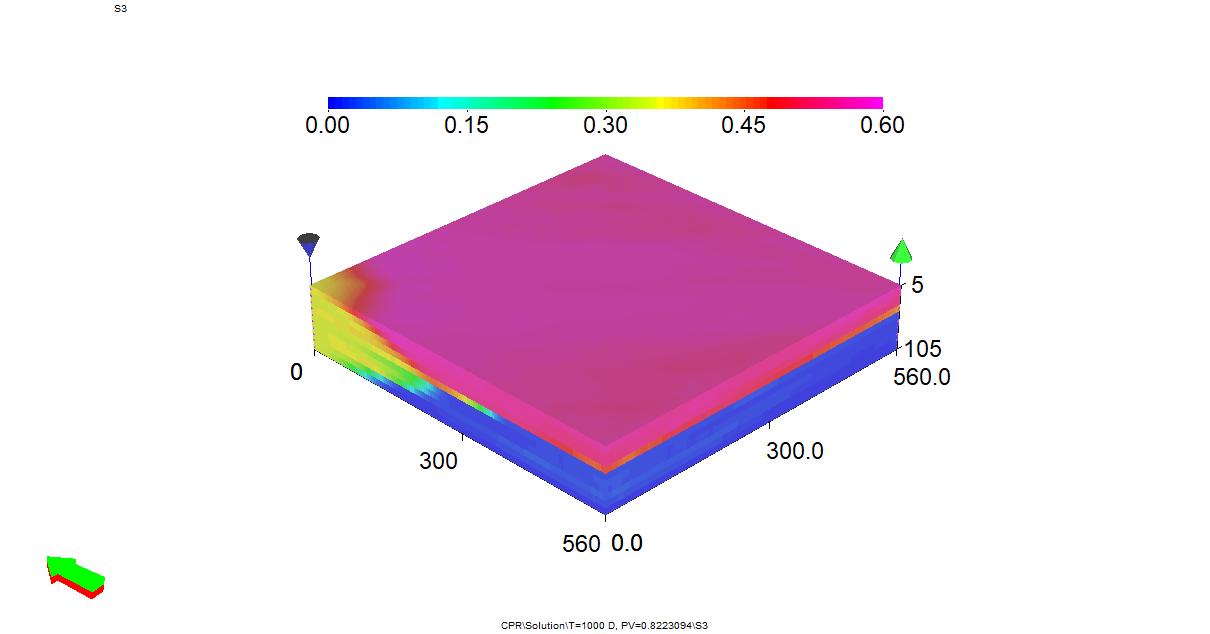
\includegraphics[width=1.3\linewidth]{figures/case1_cpr_sgas.png}
  \caption{\texttt{CPR-AMG} preconditioner.}
\end{subfigure}%
\begin{subfigure}{.5\textwidth}
  \centering
  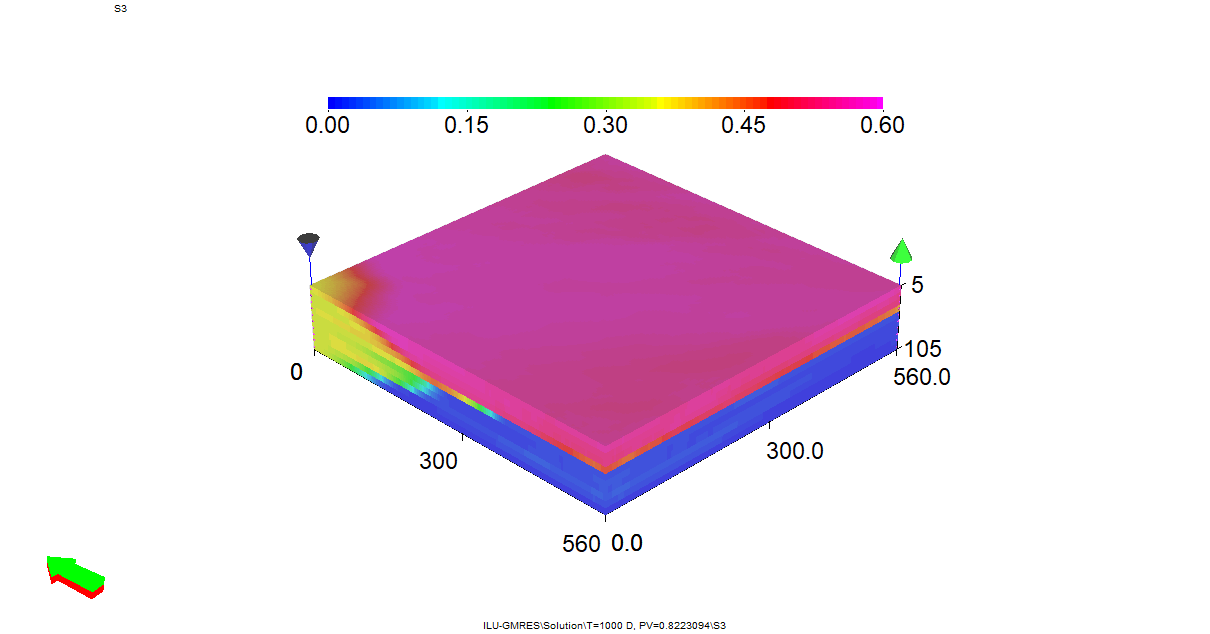
\includegraphics[width=1.3\linewidth]{figures/case1_ilu_sgas.png}
  \caption{\texttt{GMRES-ILU(0)} preconditioner}
\end{subfigure}
\caption{A comparison of \texttt{Case 1} gas saturation $S_{g}$ distribution for the two different preconditioning methods after 1000 days of simulation.}
\label{case1sg}
\end{figure}

\begin{table}[h!]
   \caption{Comparison parameters for \texttt{Case 1}.}
   \label{case1-tab}
   \small
   \centering
   \begin{tabular}{lcc}
   \toprule\toprule
   \textbf{Variable} & \textbf{CPR-AMG} & \textbf{GMRES-ILU(0)} \\
   \midrule
   CPU Time (hr) & 1.26 & 9.4 \\
   Solver Time (hr) & 0.79 & 8.97 \\
   \# Newton Iterations & 147 & 147 \\
   \# Solver Iterations & 4,025 & 107,192 \\
   \# Time Steps & 67 & 67 \\
   \bottomrule
   \end{tabular}
\end{table}

\begin{figure}
\centering
\begin{subfigure}{.5\textwidth}
  \centering
  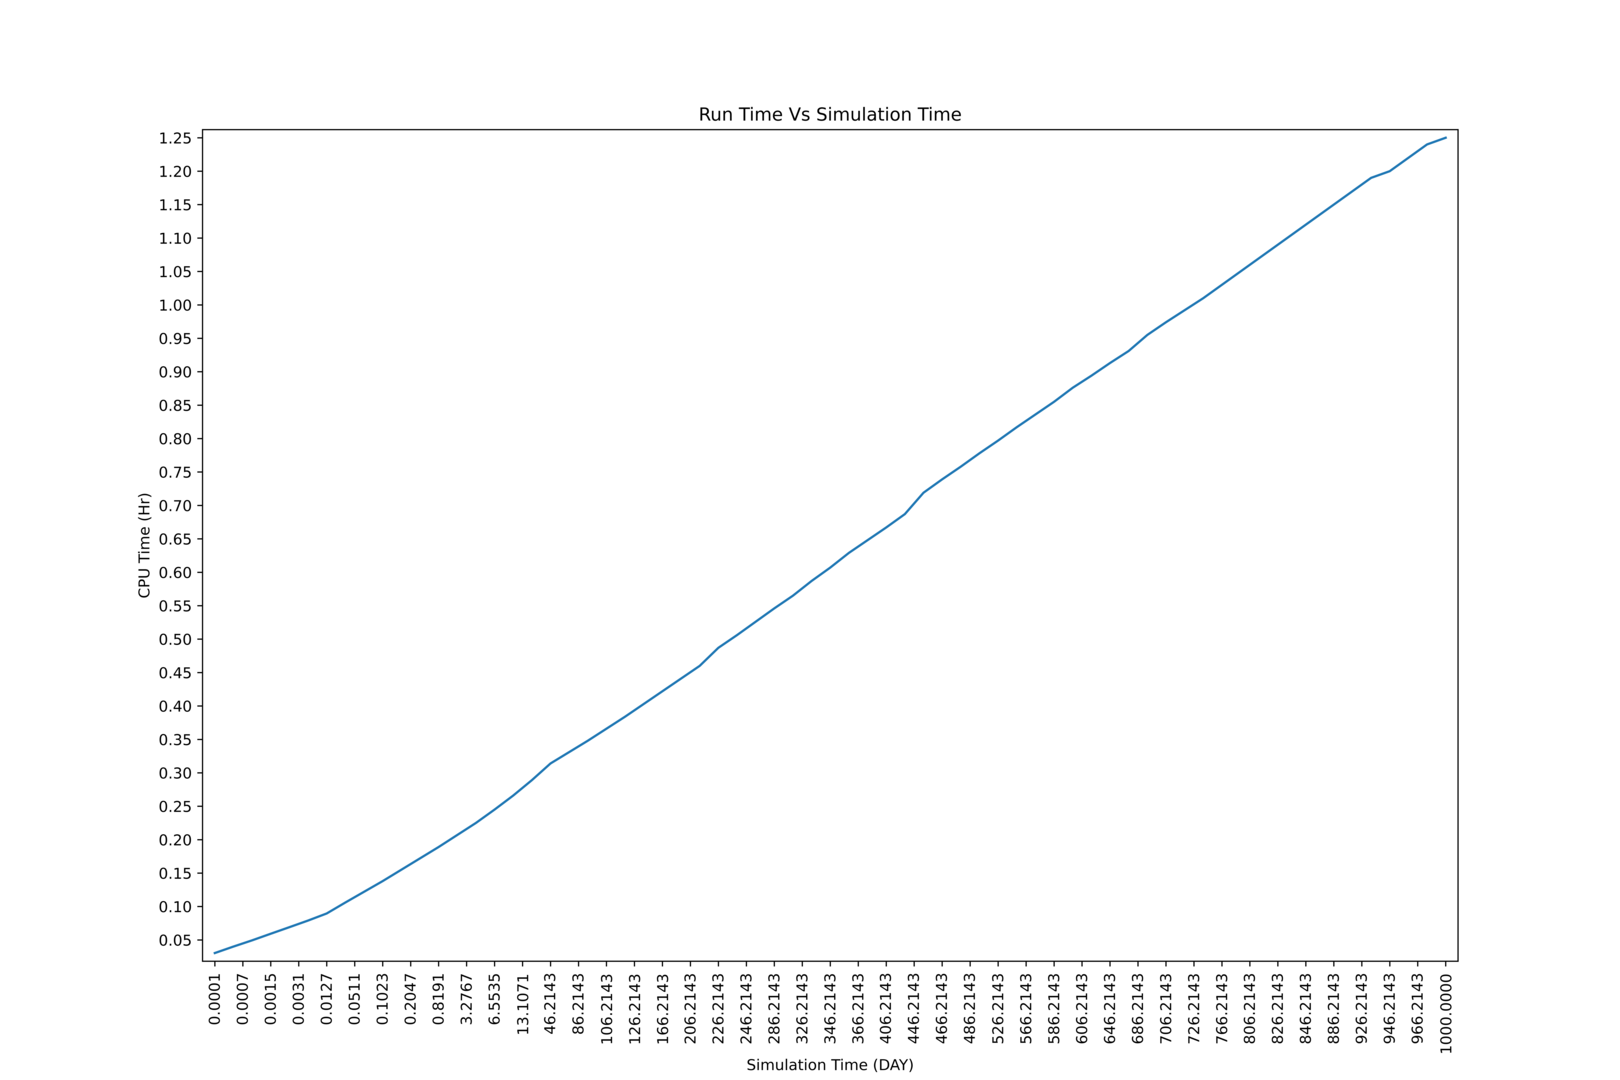
\includegraphics[width=1.1\linewidth]{figures/case1/cpr/cpu_time.png_reduced.png}
  \caption{\texttt{CPR-AMG} preconditioner.}
	\label{case1_cpu_cpr}
\end{subfigure}%
\begin{subfigure}{.5\textwidth}
  \centering
  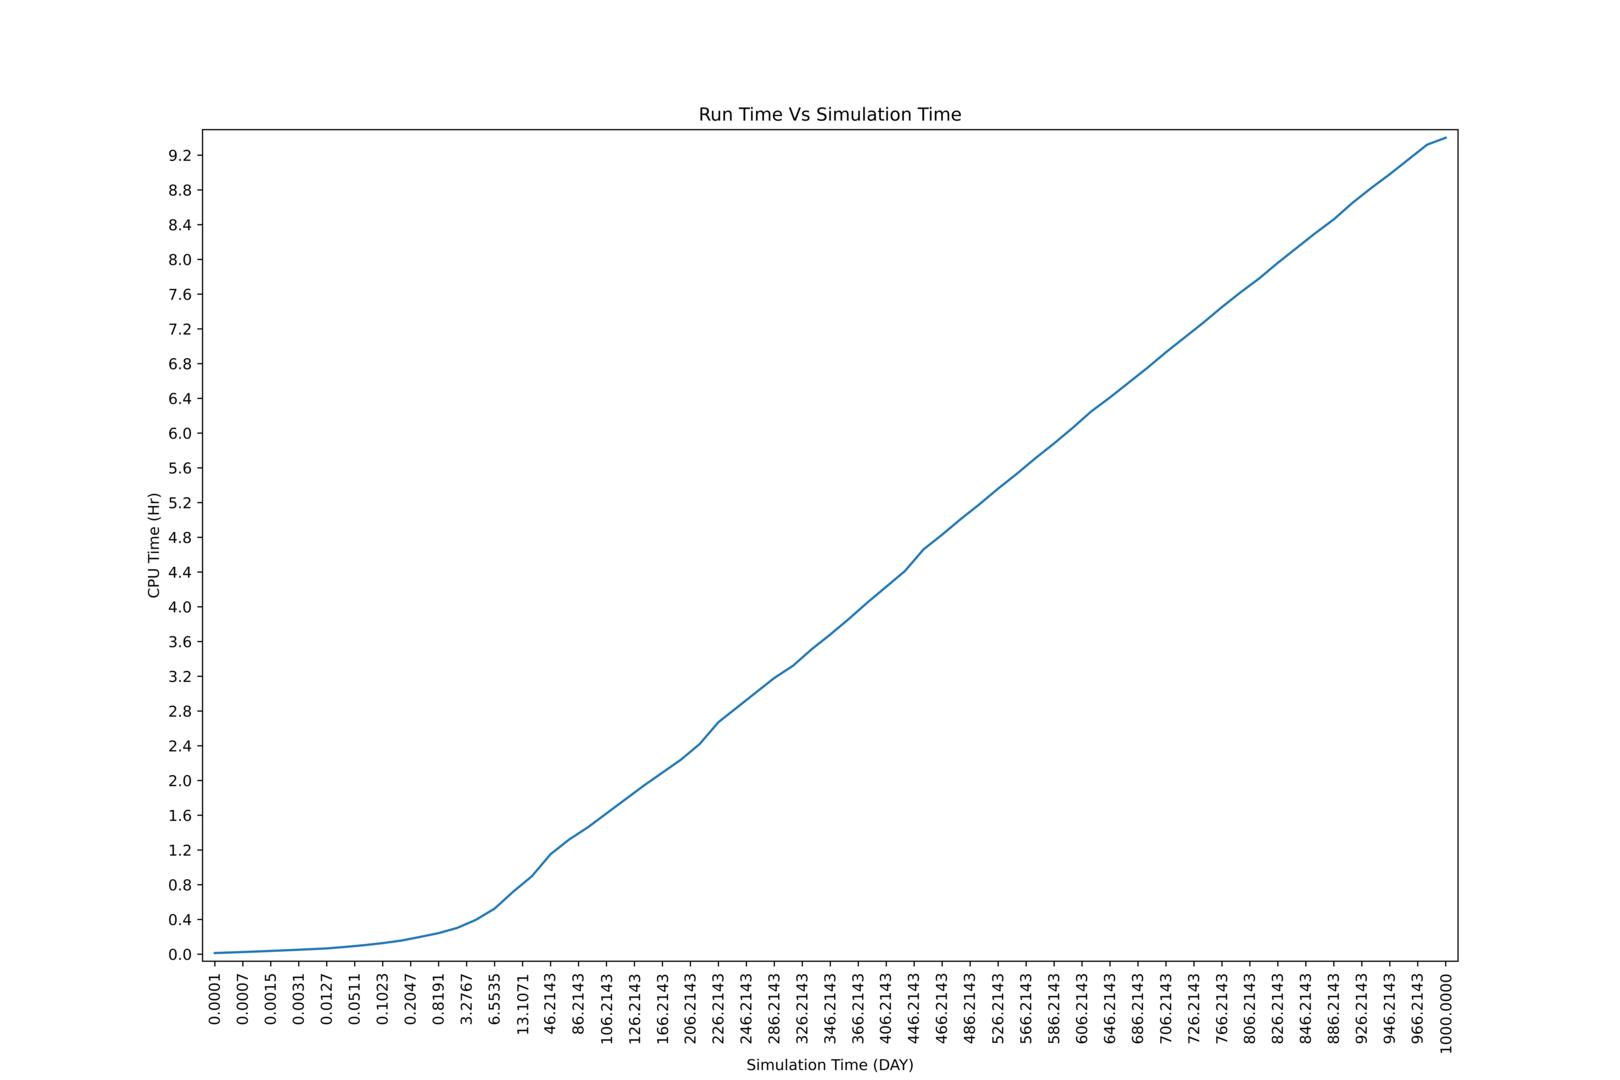
\includegraphics[width=1.1\linewidth]{figures/case1/ilu/cpu_time.png_reduced.png}
  \caption{\texttt{GMRES-ILU(0)} preconditioner}
	\label{case1_cpu_ilu}
\end{subfigure}
\begin{subfigure}{.5\textwidth}
  \centering
  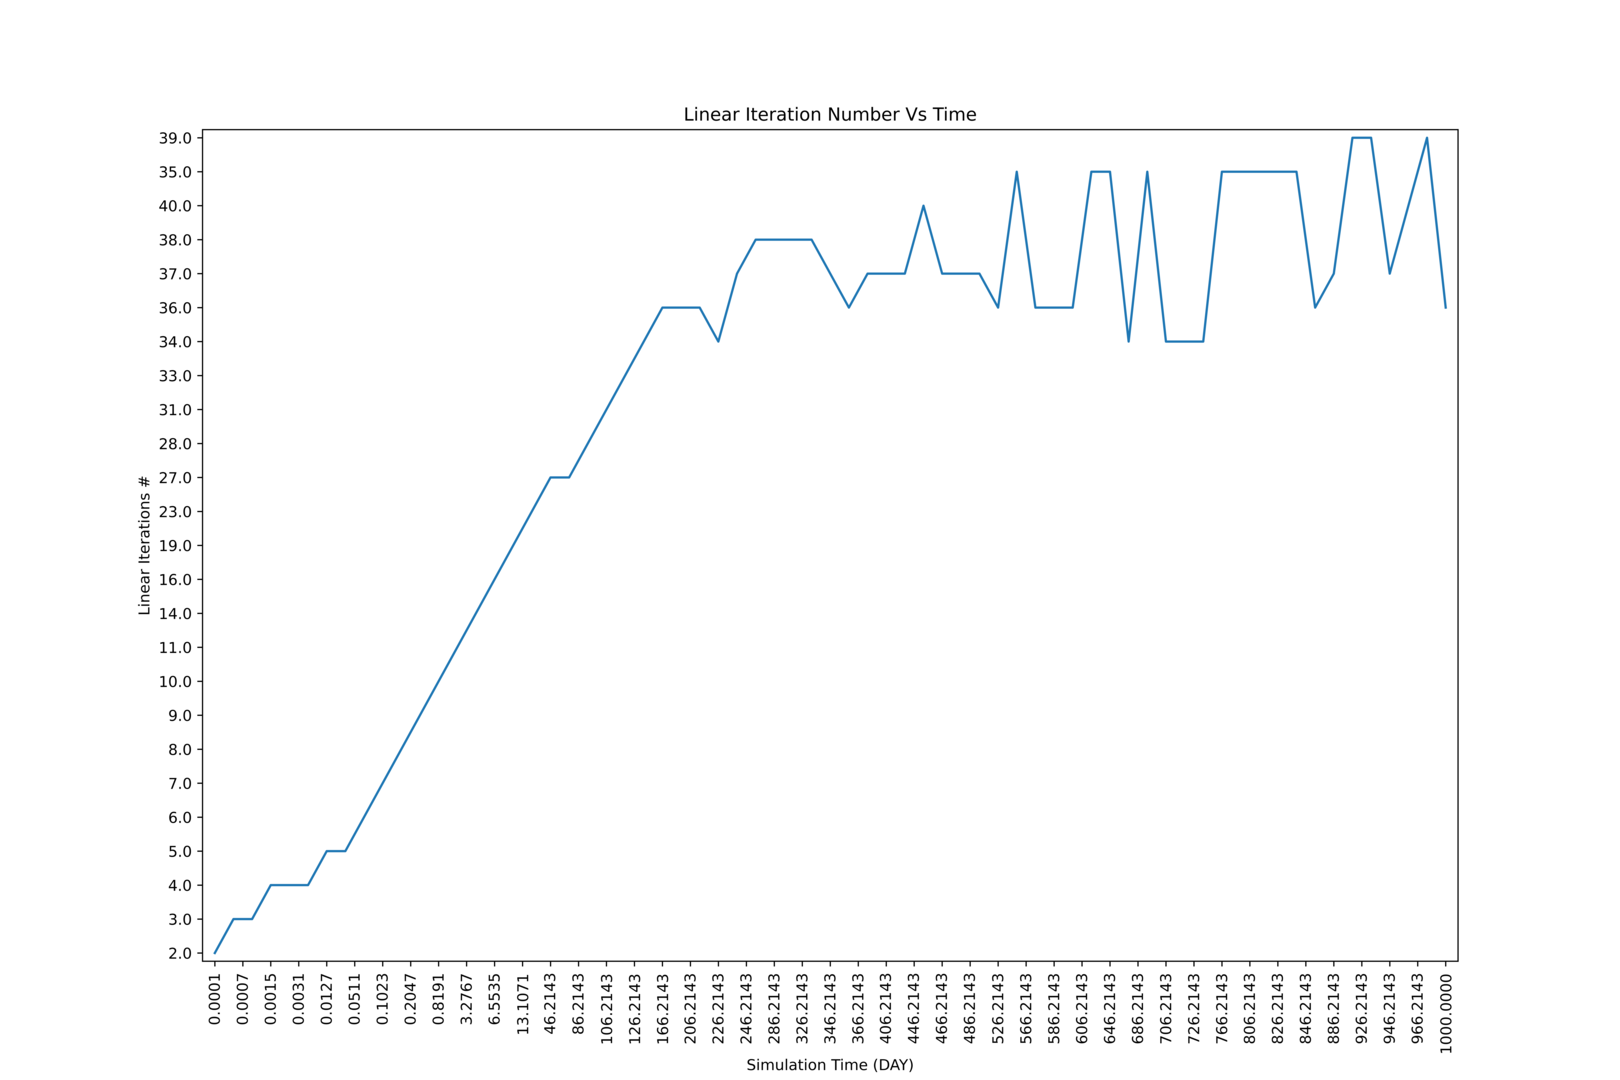
\includegraphics[width=1.1\linewidth]{figures/case1/cpr/its_time.png_reduced.png}
  \caption{\texttt{CPR-AMG} preconditioner.}
	\label{case1_its_cpr}
\end{subfigure}%
\begin{subfigure}{.5\textwidth}
  \centering
  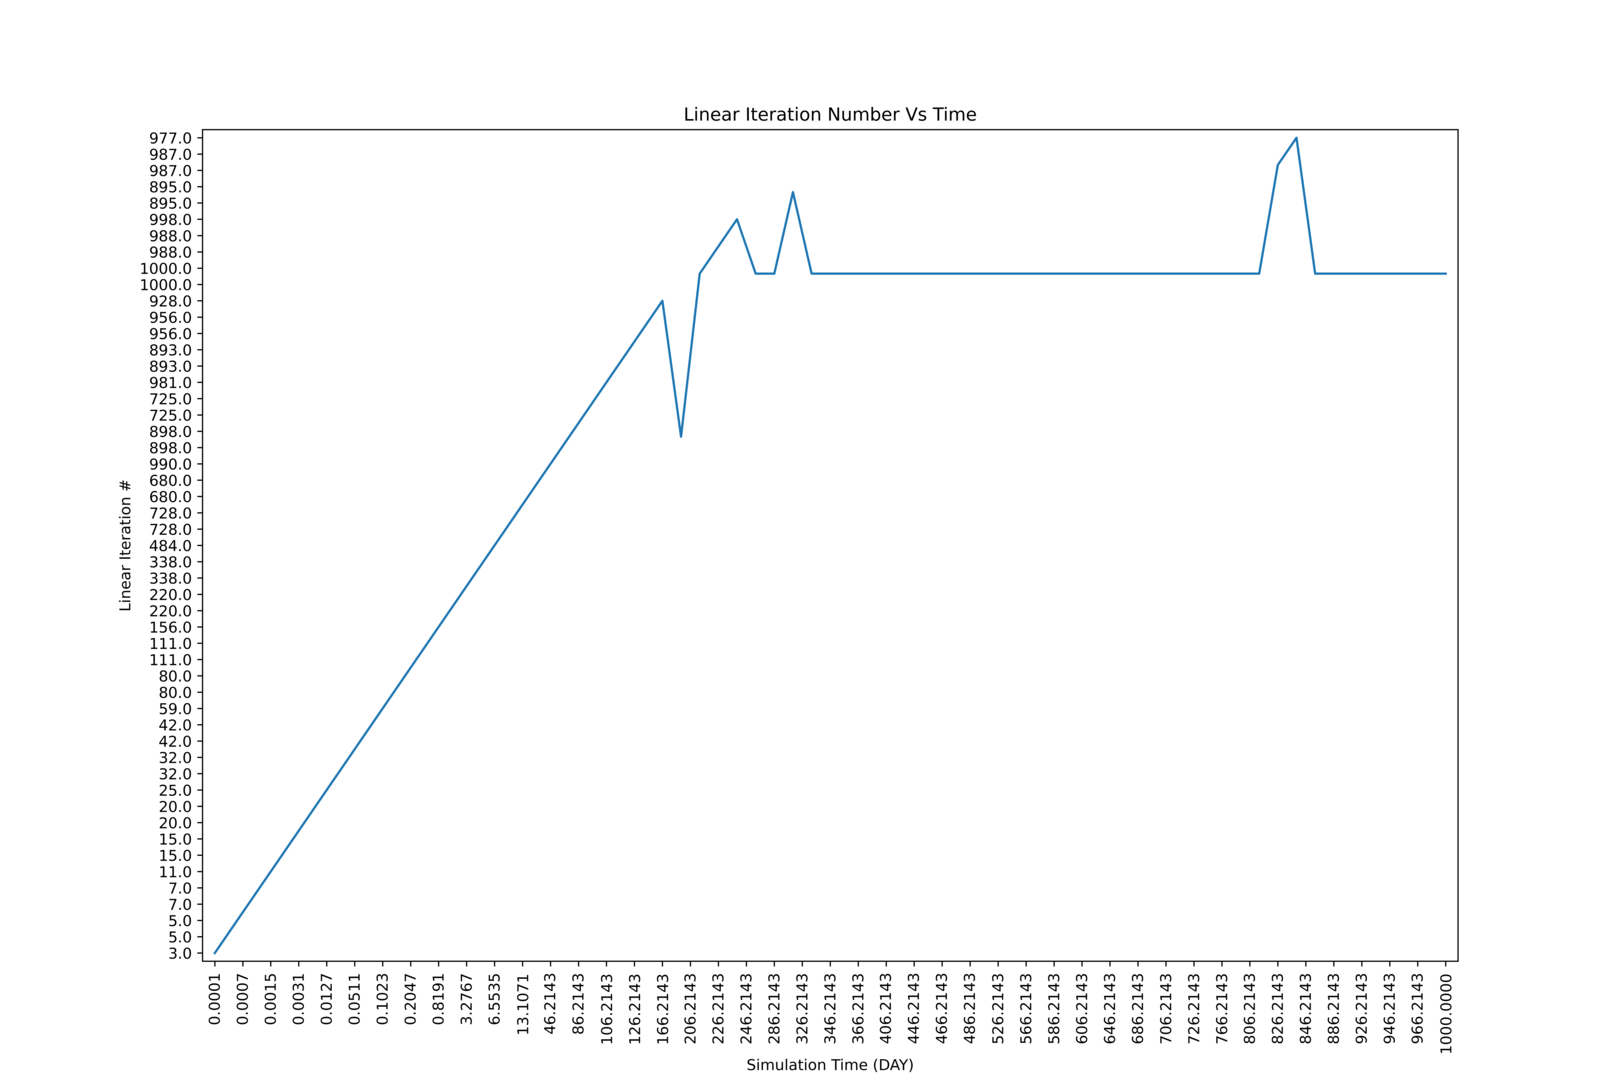
\includegraphics[width=1.1\linewidth]{figures/case1/ilu/its_time.png_reduced.png}
  \caption{\texttt{GMRES-ILU(0)} preconditioner}
	\label{case1_its_ilu}
\end{subfigure}
\begin{subfigure}{.5\textwidth}
  \centering
  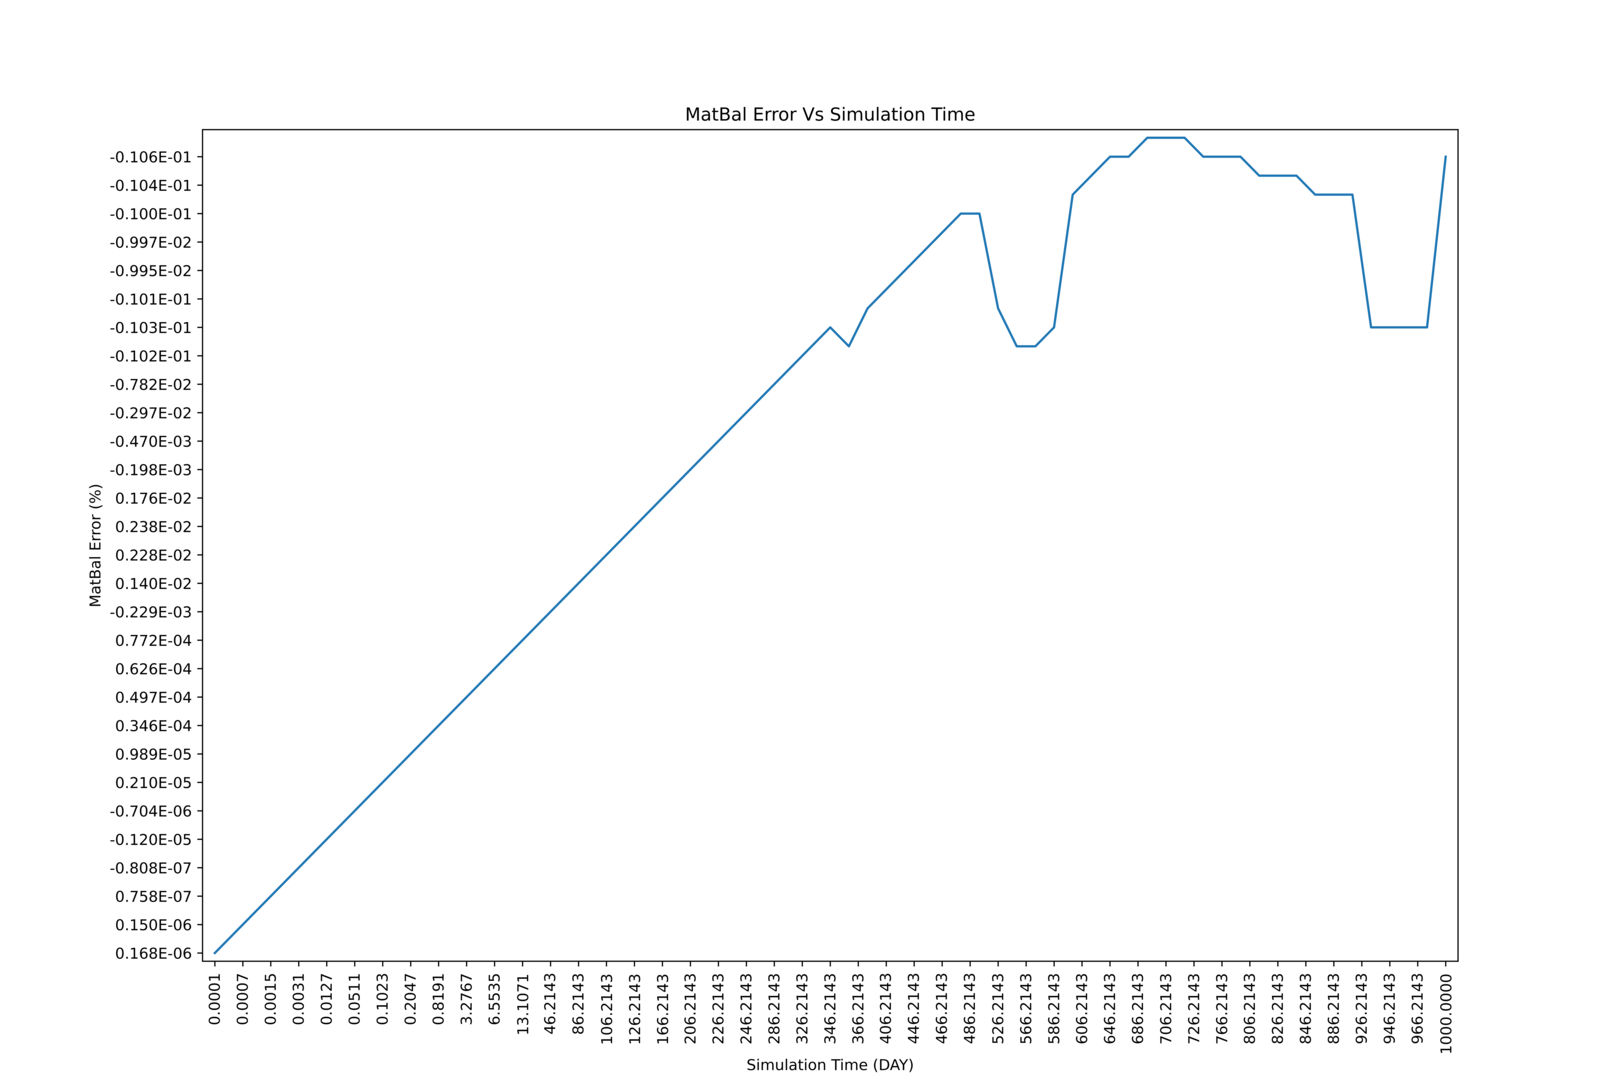
\includegraphics[width=1.1\linewidth]{figures/case1/cpr/matbalerr_time.png_reduced.png}
  \caption{\texttt{CPR-AMG} preconditioner.}
	\label{case1_matbalerr_cpr}
\end{subfigure}%
\begin{subfigure}{.5\textwidth}
  \centering
  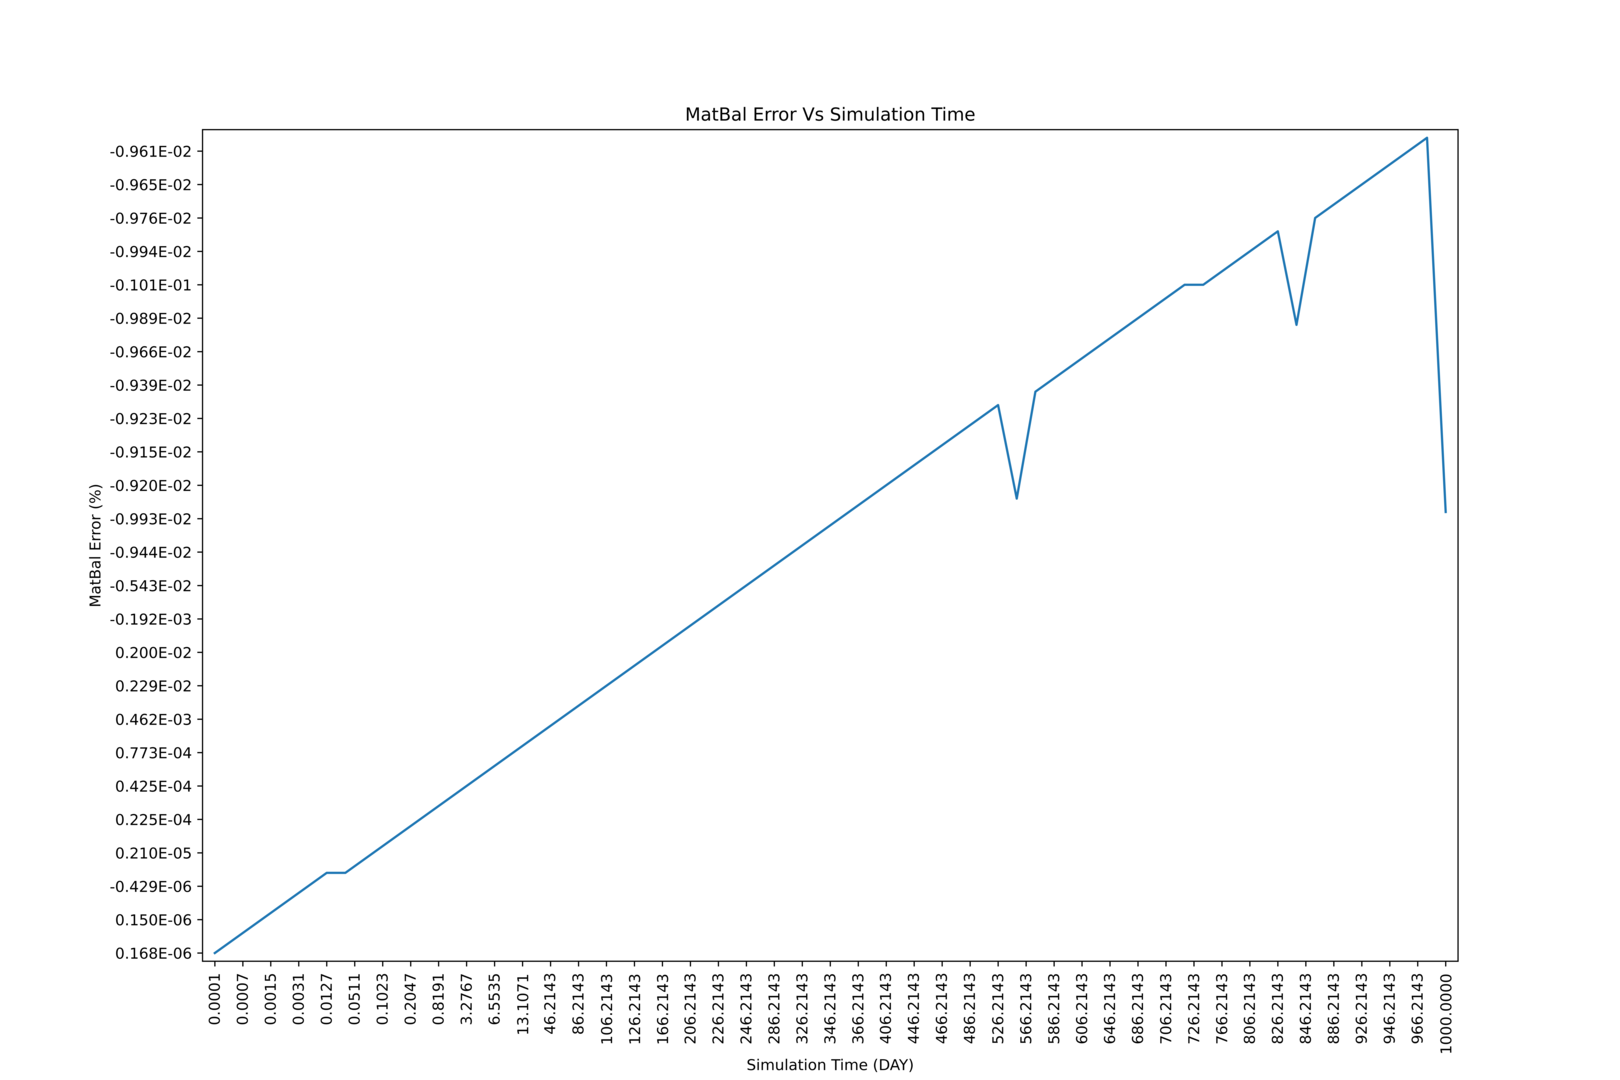
\includegraphics[width=1.1\linewidth]{figures/case1/ilu/matbalerr_time.png_reduced.png}
  \caption{\texttt{GMRES-ILU(0)} preconditioner}
	\label{case1_matbalerr_ilu}
\end{subfigure}
%\caption{A comparison for \texttt{Case 1} for the two different preconditioning methods.}
\caption[caption]{A comparison for \texttt{Case 1} for the two different preconditioning methods.\\\hspace{\textwidth}
		\cref{case1_cpu_cpr,case1_cpu_ilu}: CPU run time against simulation time. \\\hspace{\textwidth}
		\cref{case1_its_cpr,case1_its_ilu}: Linear iterations against simulation time.\\\hspace{\textwidth}
		\cref{case1_matbalerr_cpr,case1_matbalerr_ilu}: Material balance error against simulation time.}
\label{case1_param}
\end{figure}
\clearpage

\section{Case 2}

\FloatBarrier
\begin{center}
\begin{table}[h!]
\begin{adjustbox}{width=0.8\textwidth}
    \begin{threeparttable}
    \caption{\textbf{Case 2 Reservoir Parameters\supercite{fernandes}.}}
    \label{case2}
        \begin{tabular}{l r }
            \toprule
            Simulatoin Parameters & Value\\
            \midrule
	\rowcolor{red!20}\textit{\textbf{Reservoir data}}      & \\
	Grid:      &           $200\times400\times25$ ($465,816$ active) \\
	\rowcolor{blue!5}Number of wells:      &  49 (25 injectors / 24 producers) \\
	Length, width and thickness:      & $1,219.2$ m, $2,438.4$ m and $45.72$ m\\
	Initial water saturation:    & $0.17$ \\      
	\rowcolor{blue!5}Initial pressure:    &      $20.68$ MPa\\
	Formation temperature:    & $303.15$ K     \\
	Gas injection rate:    &       $86,366 \ m^{3}/d$ \\
	\rowcolor{blue!5}Producer’s bottom hole pressure:    &       $20.68$ MPa\\
	Reservoir’s initial composition ($C_{1}$, $C_{3}$ $C_{10}$): & $0.1$, $0.19$, $0.8$\\
	\rowcolor{blue!5}Injection fluid composition ($C_{1}$, $C_{3}$, $C_{10}$):    &   $0.95$, $0.05$, $0.0$\\
	\rowcolor{red!20}\textit{\textbf{Run data}}    &       \\
	Simulation time (days):    &  $2,190$\\
	\rowcolor{blue!5}Simulation time (pore volumes):    & $1.477$\\
            \bottomrule
        \end{tabular}
    \end{threeparttable}
\end{adjustbox}    
\end{table}
\end{center}
\FloatBarrier

\begin{table}[h!]
   \caption{Comparison parameters for \texttt{Case 2}.}
   \label{case2-tab}
   \small
   \centering
   \begin{tabular}{lcc}
   \toprule\toprule
   \textbf{Variable} & \textbf{CPR-AMG} & \textbf{GMRES-ILU(0)} \\
   \midrule
   CPU Time (hr) & 27.5 & 54.2 \\
   Solver Time (hr) & 21.31 & 48.42 \\
   \# Newton Iterations & 5,751 & 5,717 \\
   \# Solver Iterations & 21,821 & 177,798 \\
   \# Time Steps & 624 & 624 \\
   \bottomrule
   \end{tabular}
\end{table}

\begin{figure}
\centering
\begin{subfigure}{.5\textwidth}
  \centering
  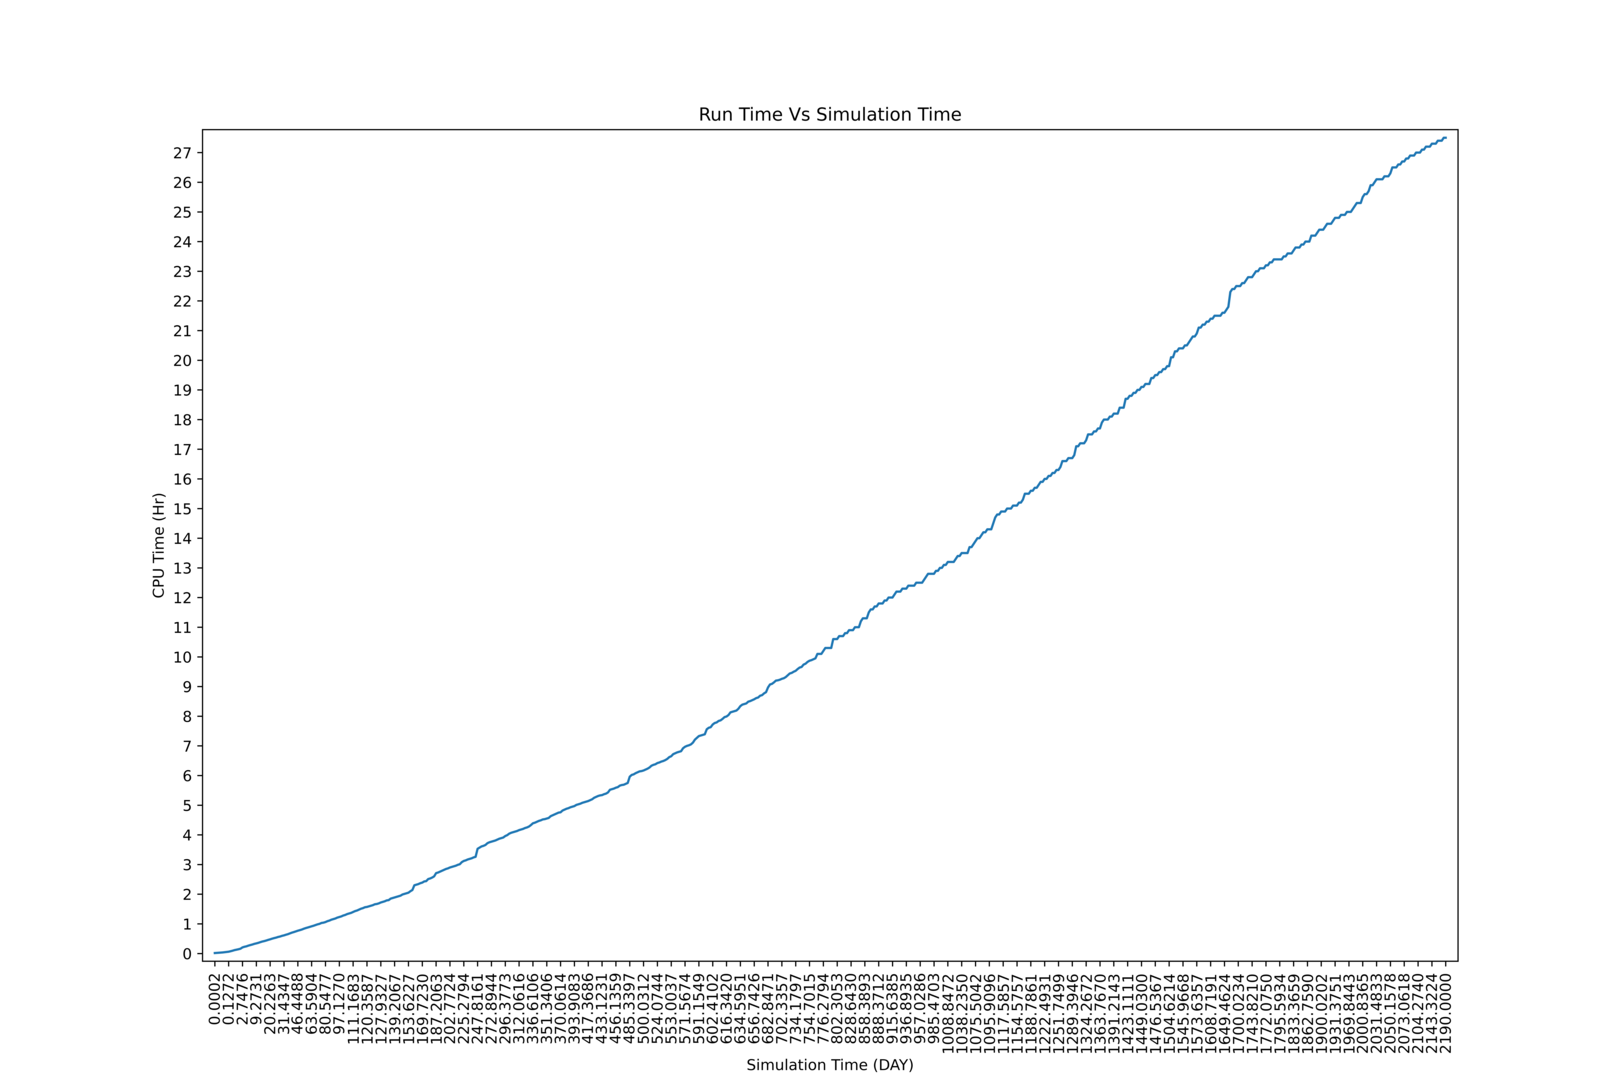
\includegraphics[width=1.1\linewidth]{figures/case2/cpr/cpu_time.png_reduced.png}
  \caption{\texttt{CPR-AMG} preconditioner.}
	\label{case2_cpu_cpr}
\end{subfigure}%
\begin{subfigure}{.5\textwidth}
  \centering
  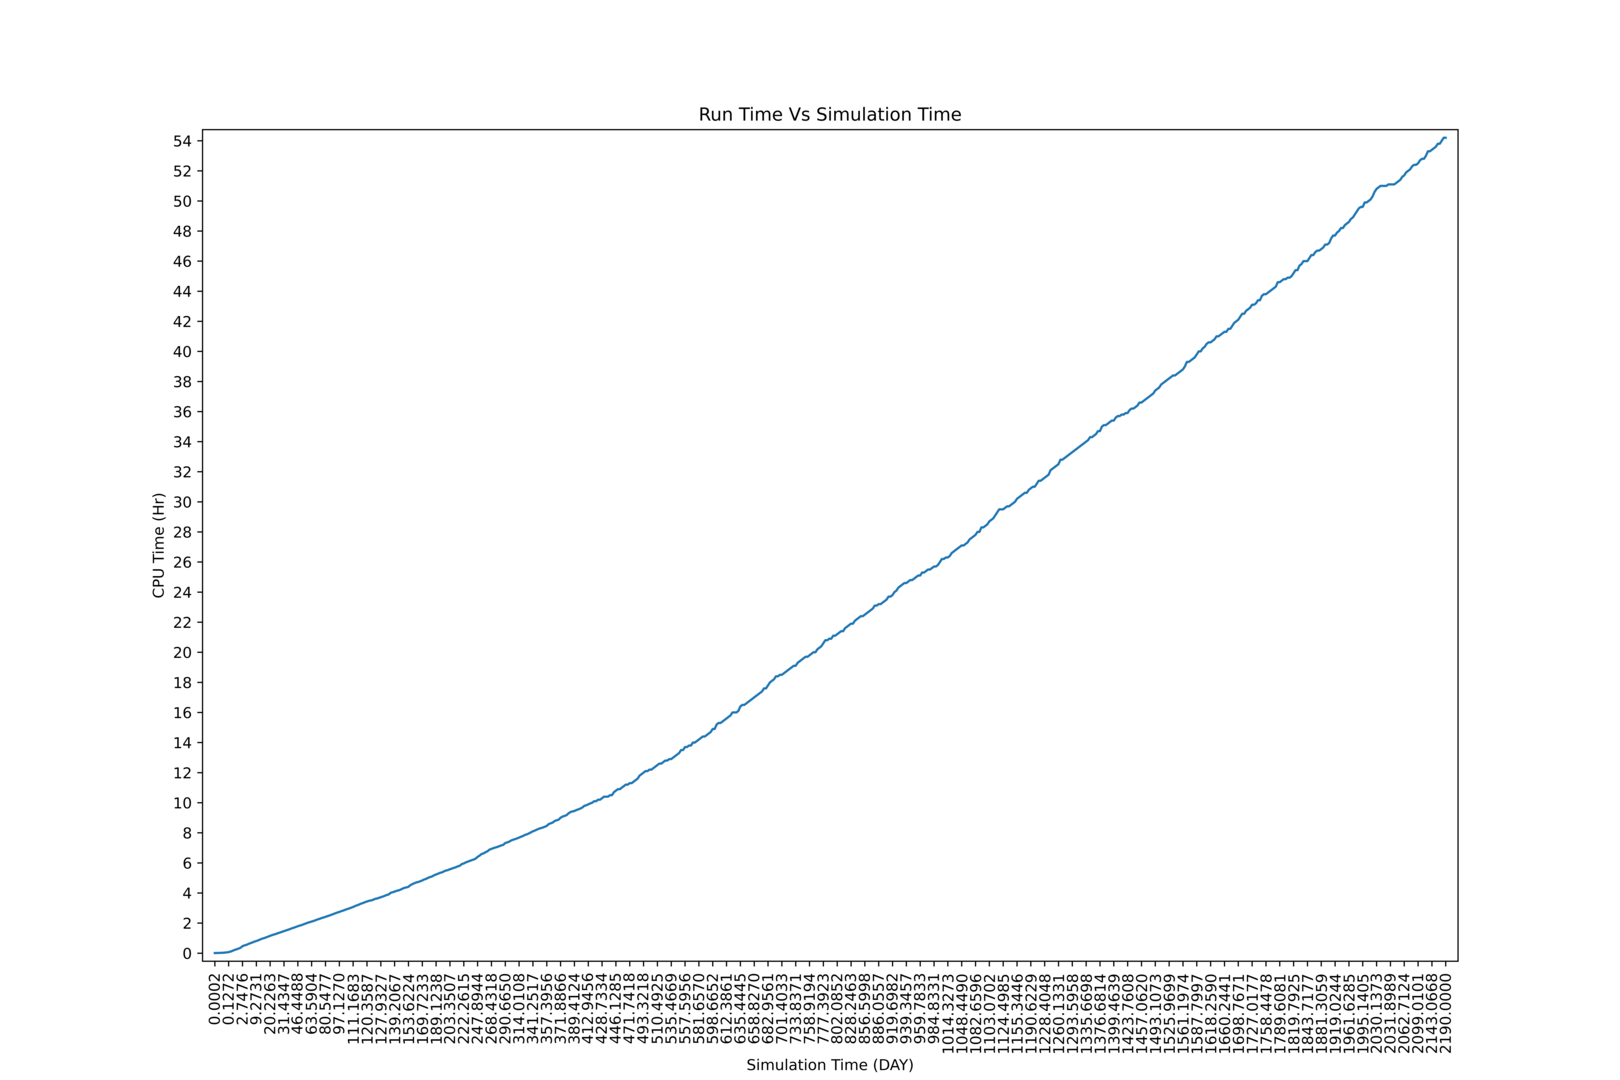
\includegraphics[width=1.1\linewidth]{figures/case2/ilu/cpu_time.png_reduced.png}
  \caption{\texttt{GMRES-ILU(0)} preconditioner}
	\label{case2_cpu_ilu}
\end{subfigure}
\begin{subfigure}{.5\textwidth}
  \centering
  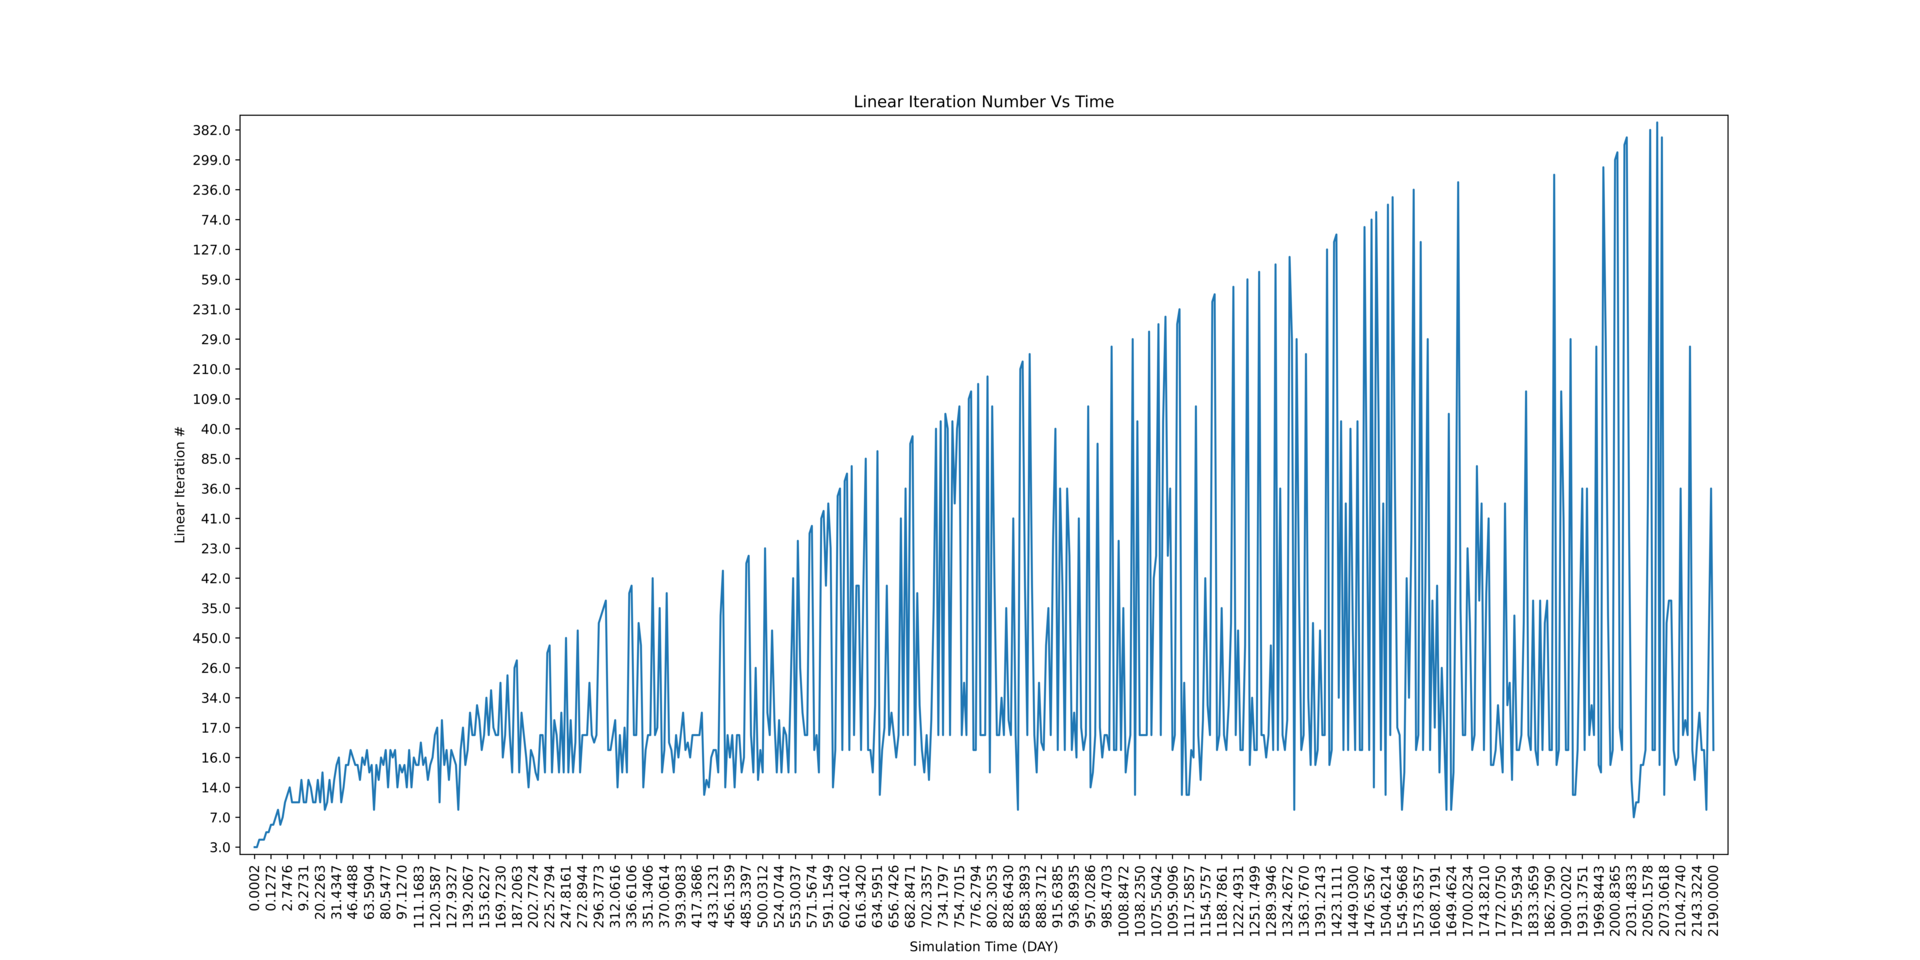
\includegraphics[width=1.1\linewidth]{figures/case2/cpr/its_time.png_reduced.png}
  \caption{\texttt{CPR-AMG} preconditioner.}
	\label{case2_its_cpr}
\end{subfigure}%
\begin{subfigure}{.5\textwidth}
  \centering
  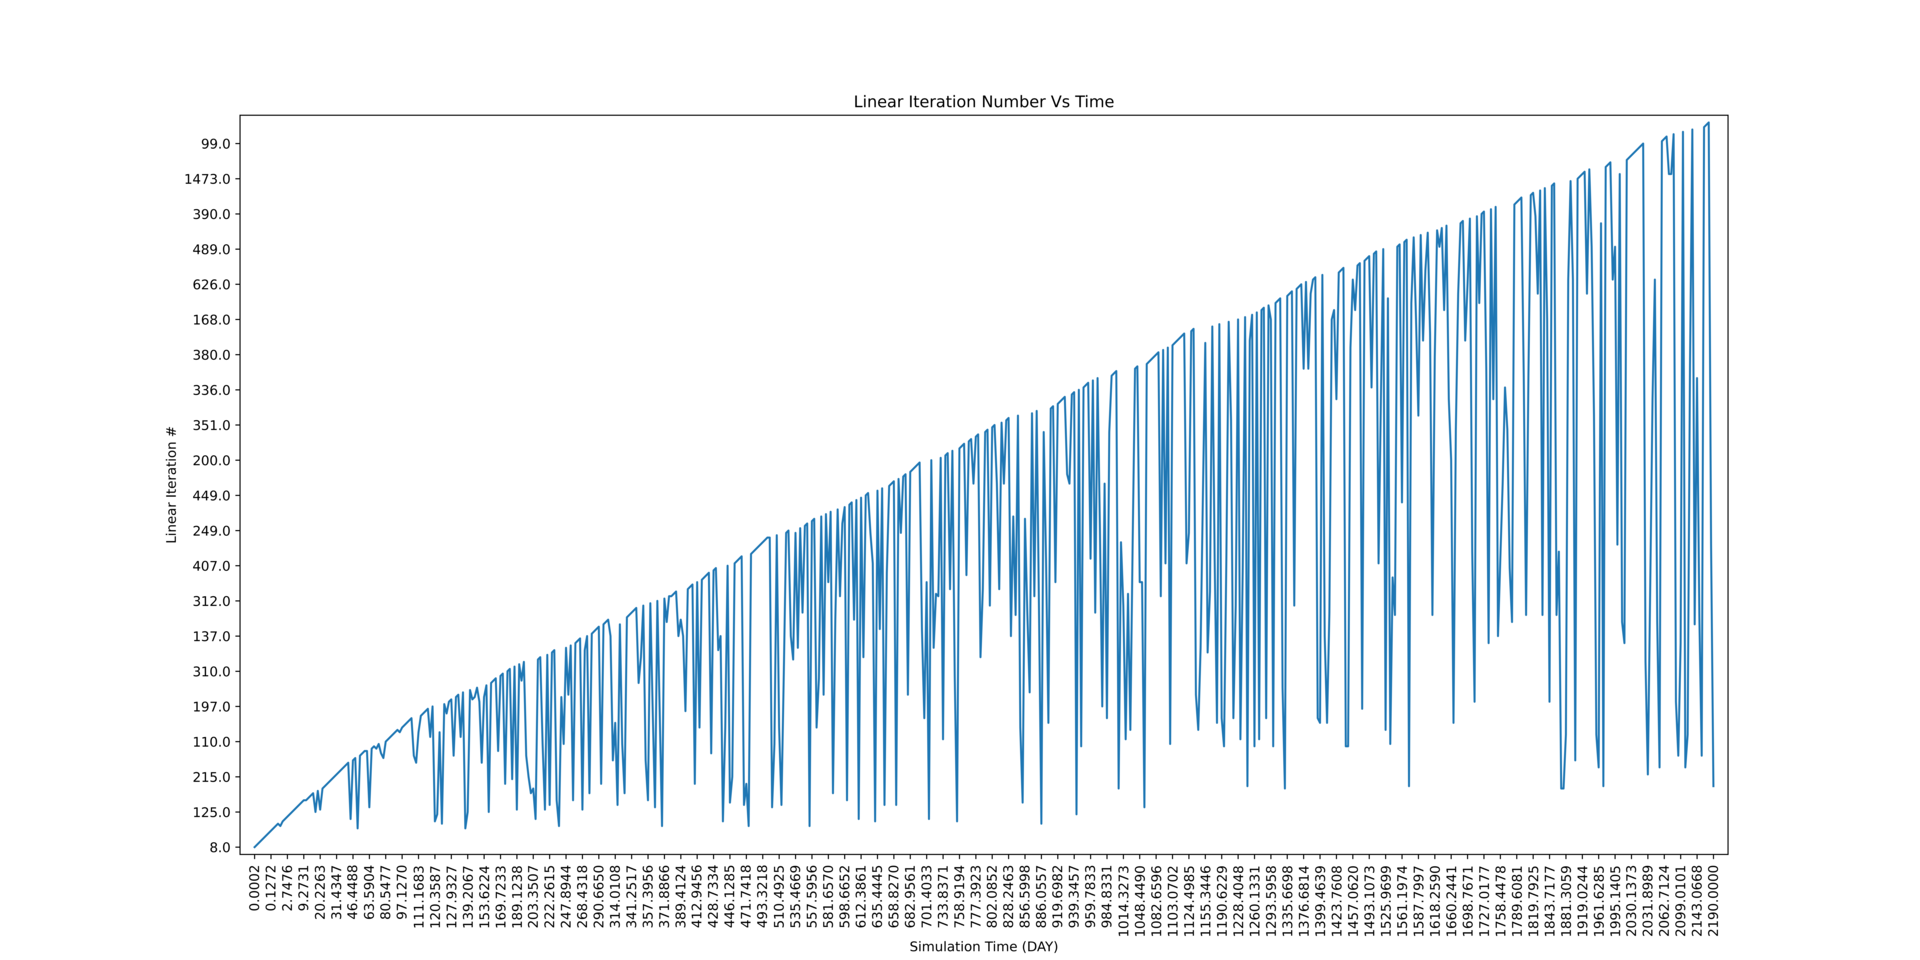
\includegraphics[width=1.1\linewidth]{figures/case2/ilu/its_time.png_reduced.png}
  \caption{\texttt{GMRES-ILU(0)} preconditioner}
	\label{case2_its_ilu}
\end{subfigure}
\begin{subfigure}{.5\textwidth}
  \centering
  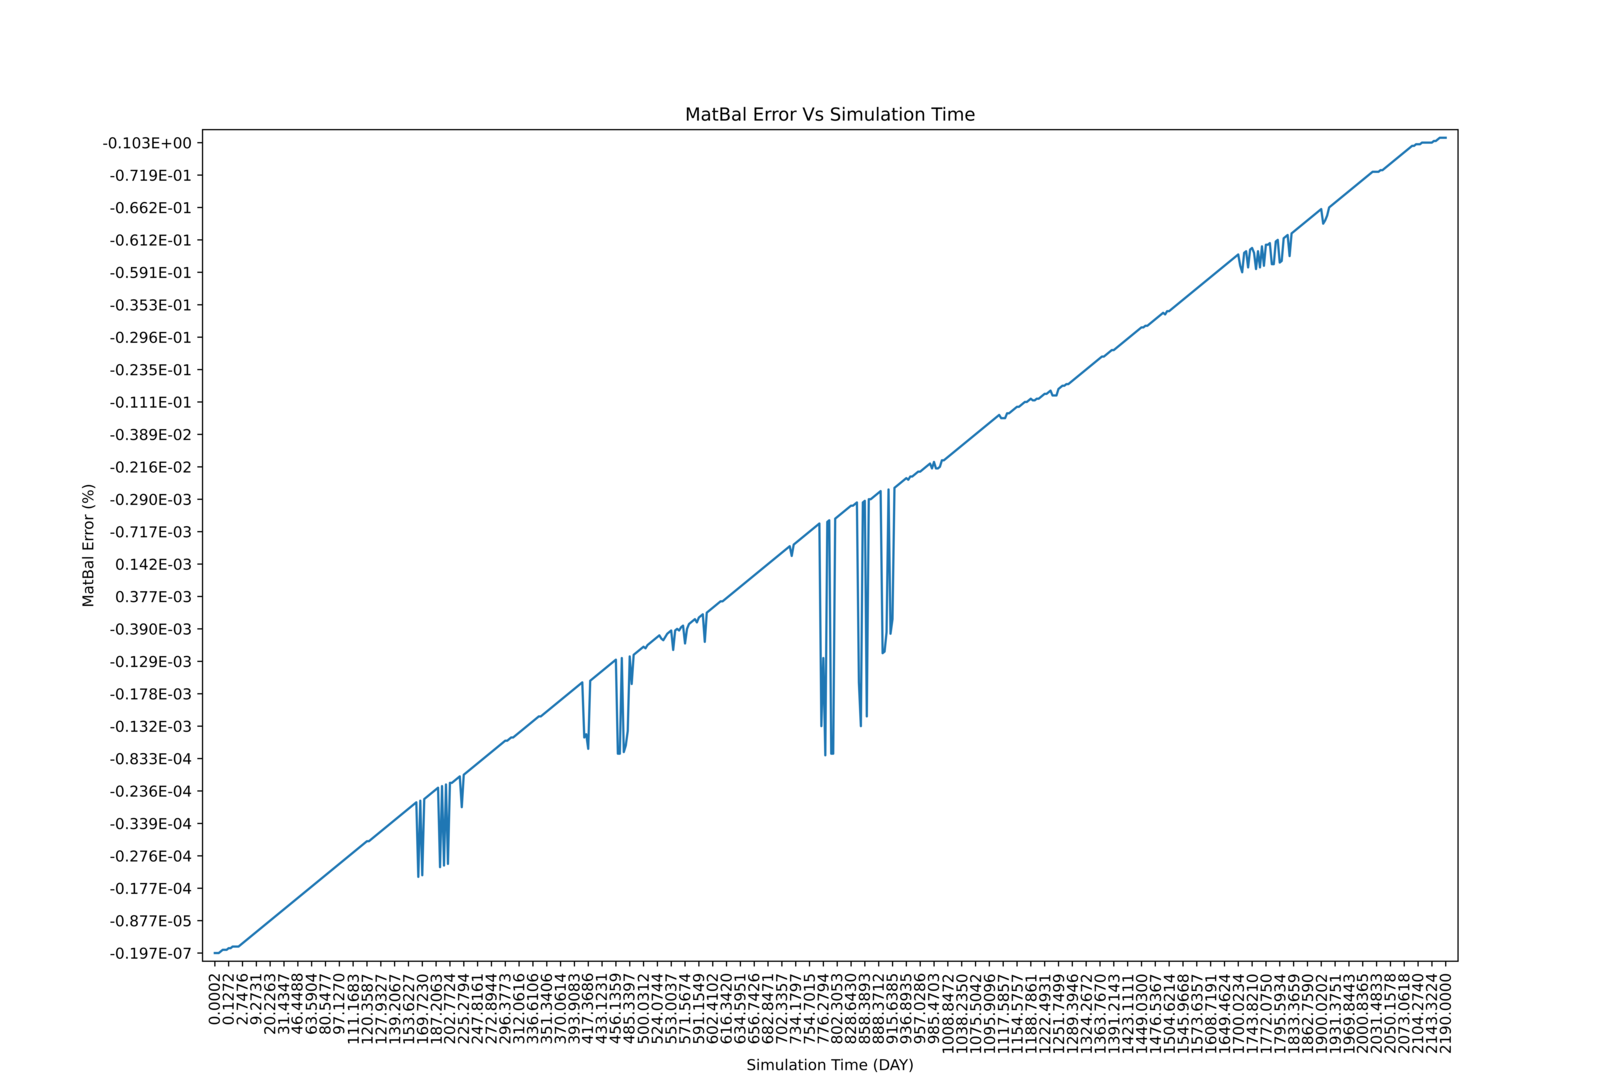
\includegraphics[width=1.1\linewidth]{figures/case2/cpr/matbalerr_time.png_reduced.png}
  \caption{\texttt{CPR-AMG} preconditioner.}
	\label{case2_matbalerr_cpr}
\end{subfigure}%
\begin{subfigure}{.5\textwidth}
  \centering
  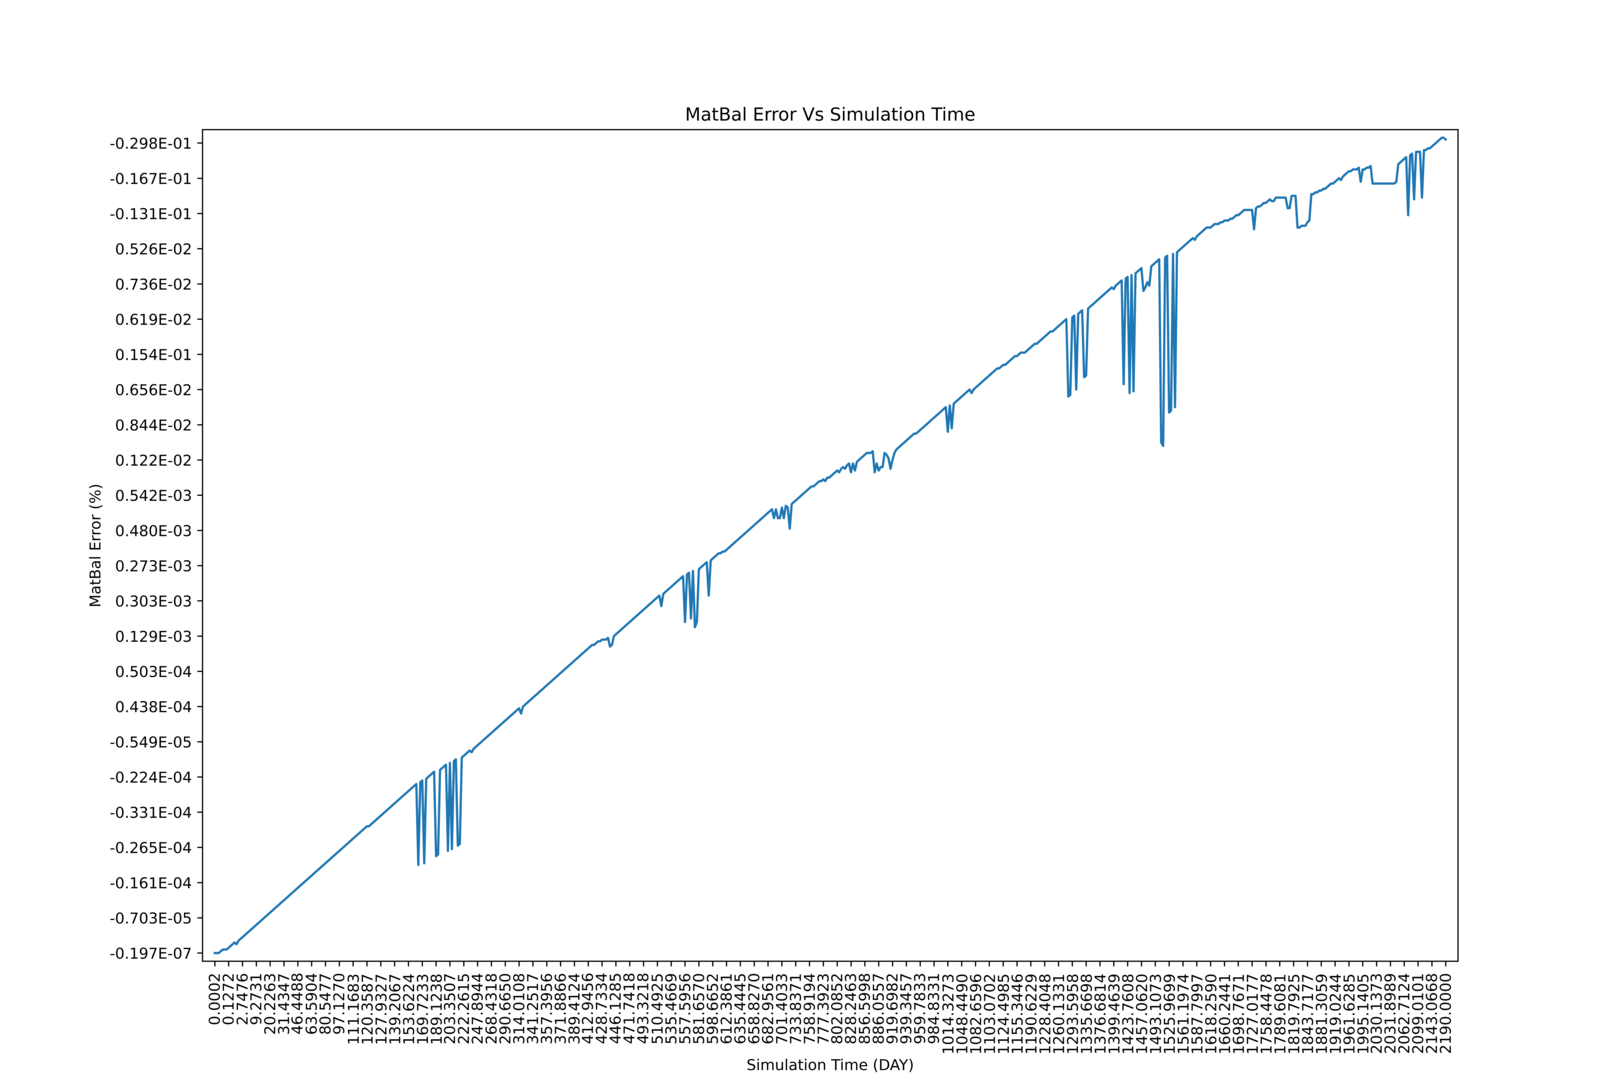
\includegraphics[width=1.1\linewidth]{figures/case2/ilu/matbalerr_time.png_reduced.png}
  \caption{\texttt{GMRES-ILU(0)} preconditioner}
	\label{case2_matbalerr_ilu}
\end{subfigure}
\caption[caption]{A comparison for \texttt{Case 2} for the two different preconditioning methods.\\\hspace{\textwidth}
		\cref{case2_cpu_cpr,case2_cpu_ilu}: CPU run time against simulation time. \\\hspace{\textwidth}
		\cref{case2_its_cpr,case2_its_ilu}: Linear iterations against simulation time.\\\hspace{\textwidth}
		\cref{case2_matbalerr_cpr,case2_matbalerr_ilu}: Material balance error against simulation time.}
\label{case2_param}
\end{figure}
\clearpage

\section{Case 3}

\FloatBarrier
\begin{center}
\begin{table}[h!]
\begin{adjustbox}{width=\textwidth}
    \begin{threeparttable}
    \caption{\textbf{Case 3 Reservoir Parameters\supercite{fernandes}.}}
    \label{case3}
        \begin{tabular}{l r }
            \toprule
            Simulatoin Parameters & Value\\
            \midrule
	\rowcolor{red!20}\textit{\textbf{Reservoir data}}      & \\
	Grid:      &           $200\times200\times10$ ($99,816$ active) \\
	\rowcolor{blue!5}Number of wells:      &  2 (1 injector / 1 producer) \\
	Length, width and thickness:      & $152.4$ m, $304.8$ m and $6.096$ m\\
	\rowcolor{blue!5}Porosity:       &          $0.25$ \\
	Initial water saturation:    & $0.35$ \\      
	\rowcolor{blue!5}Initial pressure:    &      $7.58$ MPa\\
	Formation temperature:    & $313.71$ K     \\
	injector's bottom hole pressure:    &       $8.62$ MPa \\
	\rowcolor{blue!5}Producer’s bottom hole pressure:    &       $7.58$ MPa\\
	Reservoir’s initial composition ($CO_{2}$, $C_{1}$, $C_{2-3}$, $C_{4-6}$, $C_{7-15}$, $C_{16-27}$, $C_{28+}$) & $0.0337$, $0.0861$, $0.1503$, $0.1671$, $0.3304$, $0.1611$ and $0.0713$\\
	\rowcolor{blue!5}Injection fluid composition ($CO_{2}$, $C_{1}$):    &   $0.95$, $0.05$\\
        \bottomrule
        \end{tabular}
    \end{threeparttable}
\end{adjustbox}    
\end{table}
\end{center}
\FloatBarrier

\begin{table}[h!]
   \caption{Comparison parameters for \texttt{Case 3}.}
   \label{case3-tab}
   \small
   \centering
   \begin{tabular}{lcc}
   \toprule\toprule
   \textbf{Variable} & \textbf{CPR-AMG} & \textbf{GMRES-ILU(0)} \\
   \midrule
   CPU Time (hr) & 4.58 & 6.71 \\
   Solver Time (hr) & 1.7 & 3.89 \\
   \# Newton Iterations & 1,463 & 1,438 \\
   \# Solver Iterations & 5,152 & 24,068\\
   \# Time Steps & 451 & 454 \\
   \bottomrule
   \end{tabular}
\end{table}

\begin{figure}
\centering
\begin{subfigure}{.5\textwidth}
  \centering
  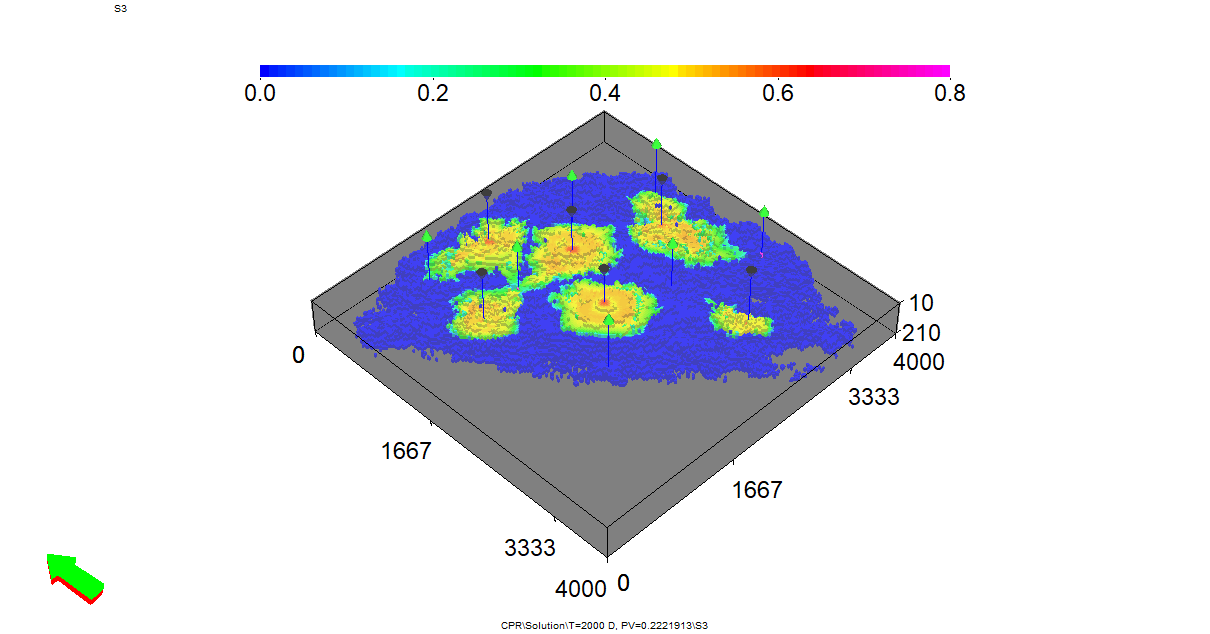
\includegraphics[width=1.3\linewidth]{figures/case3_cpr_sgas.png}
  \caption{\texttt{CPR-AMG} preconditioner.}
\end{subfigure}%
\begin{subfigure}{.5\textwidth}
  \centering
  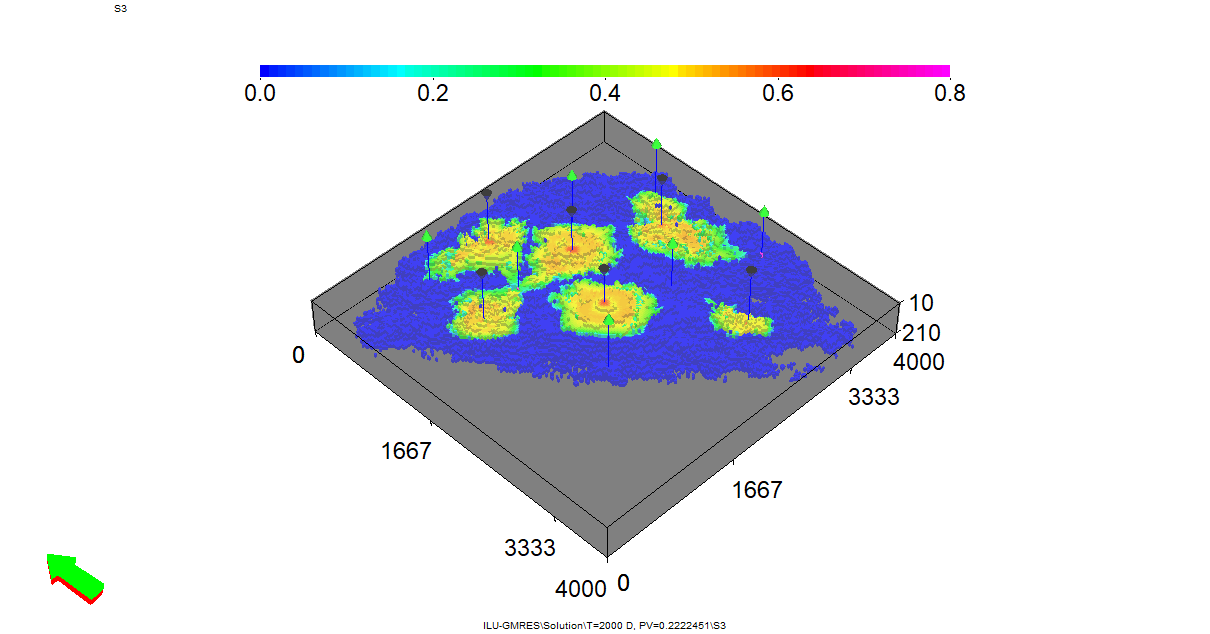
\includegraphics[width=1.3\linewidth]{figures/case3_ilu_sgas.png}
  \caption{\texttt{GMRES-ILU(0)} preconditioner}
\end{subfigure}
\caption{A comparison of \texttt{Case 3} gas saturation $S_{g}$ distribution for the two different preconditioning methods after 2000 days of simulation.}
\label{case3sg}
\end{figure}

\begin{figure}
\centering
\begin{subfigure}{.5\textwidth}
  \centering
  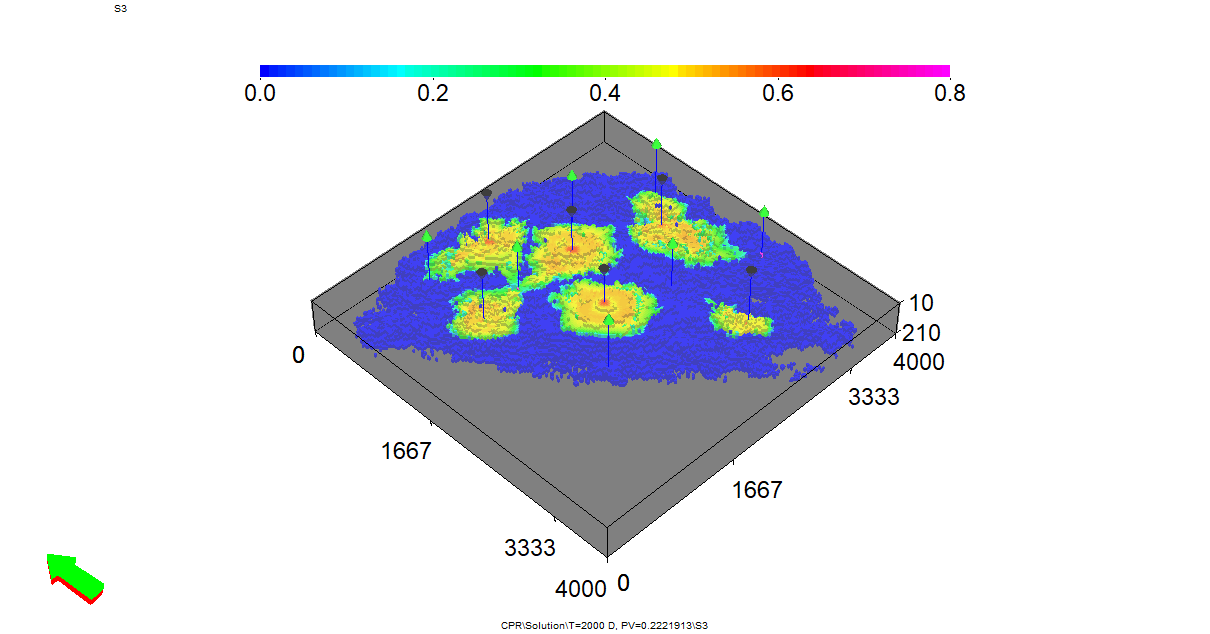
\includegraphics[width=1.3\linewidth]{figures/case3_cpr_sgas.png}
  \caption{\texttt{CPR-AMG} preconditioner.}
\end{subfigure}%
\begin{subfigure}{.5\textwidth}
  \centering
  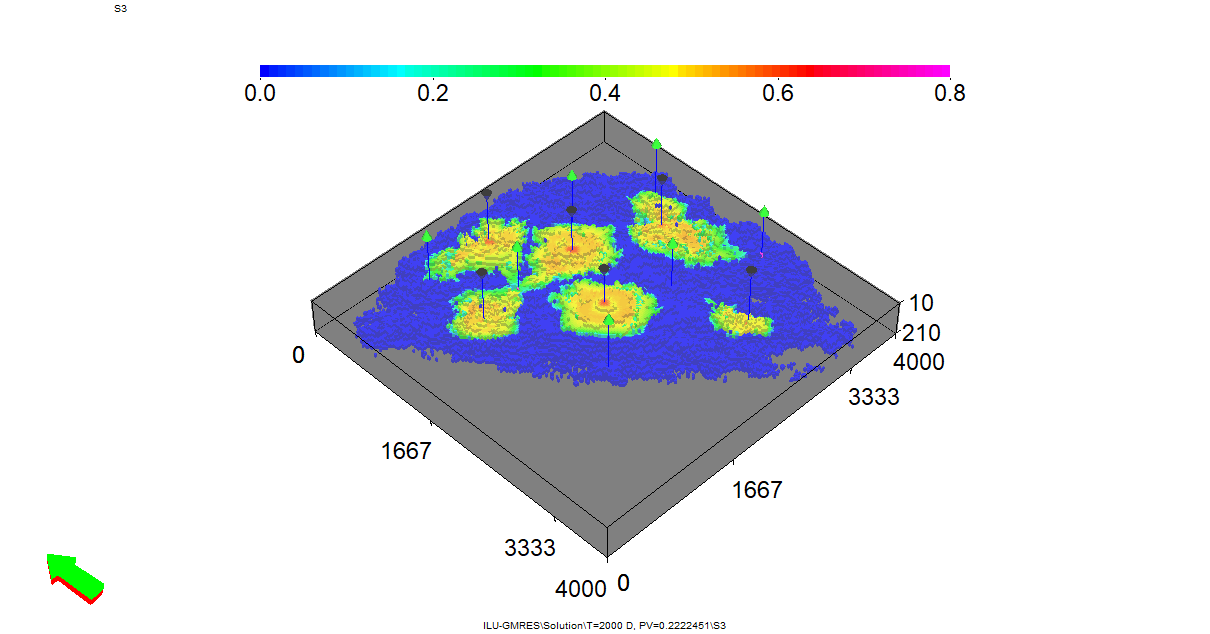
\includegraphics[width=1.3\linewidth]{figures/case3_ilu_sgas.png}
  \caption{\texttt{GMRES-ILU(0)} preconditioner}
\end{subfigure}
\caption{A comparison of \texttt{Case 3} $CO_{2}$ overall composition $Z_{CO_{2}}$ distribution for the two different preconditioning methods after 2000 days of simulation.}
\label{case3z}
\end{figure}

\begin{figure}
\centering
\begin{subfigure}{.5\textwidth}
  \centering
  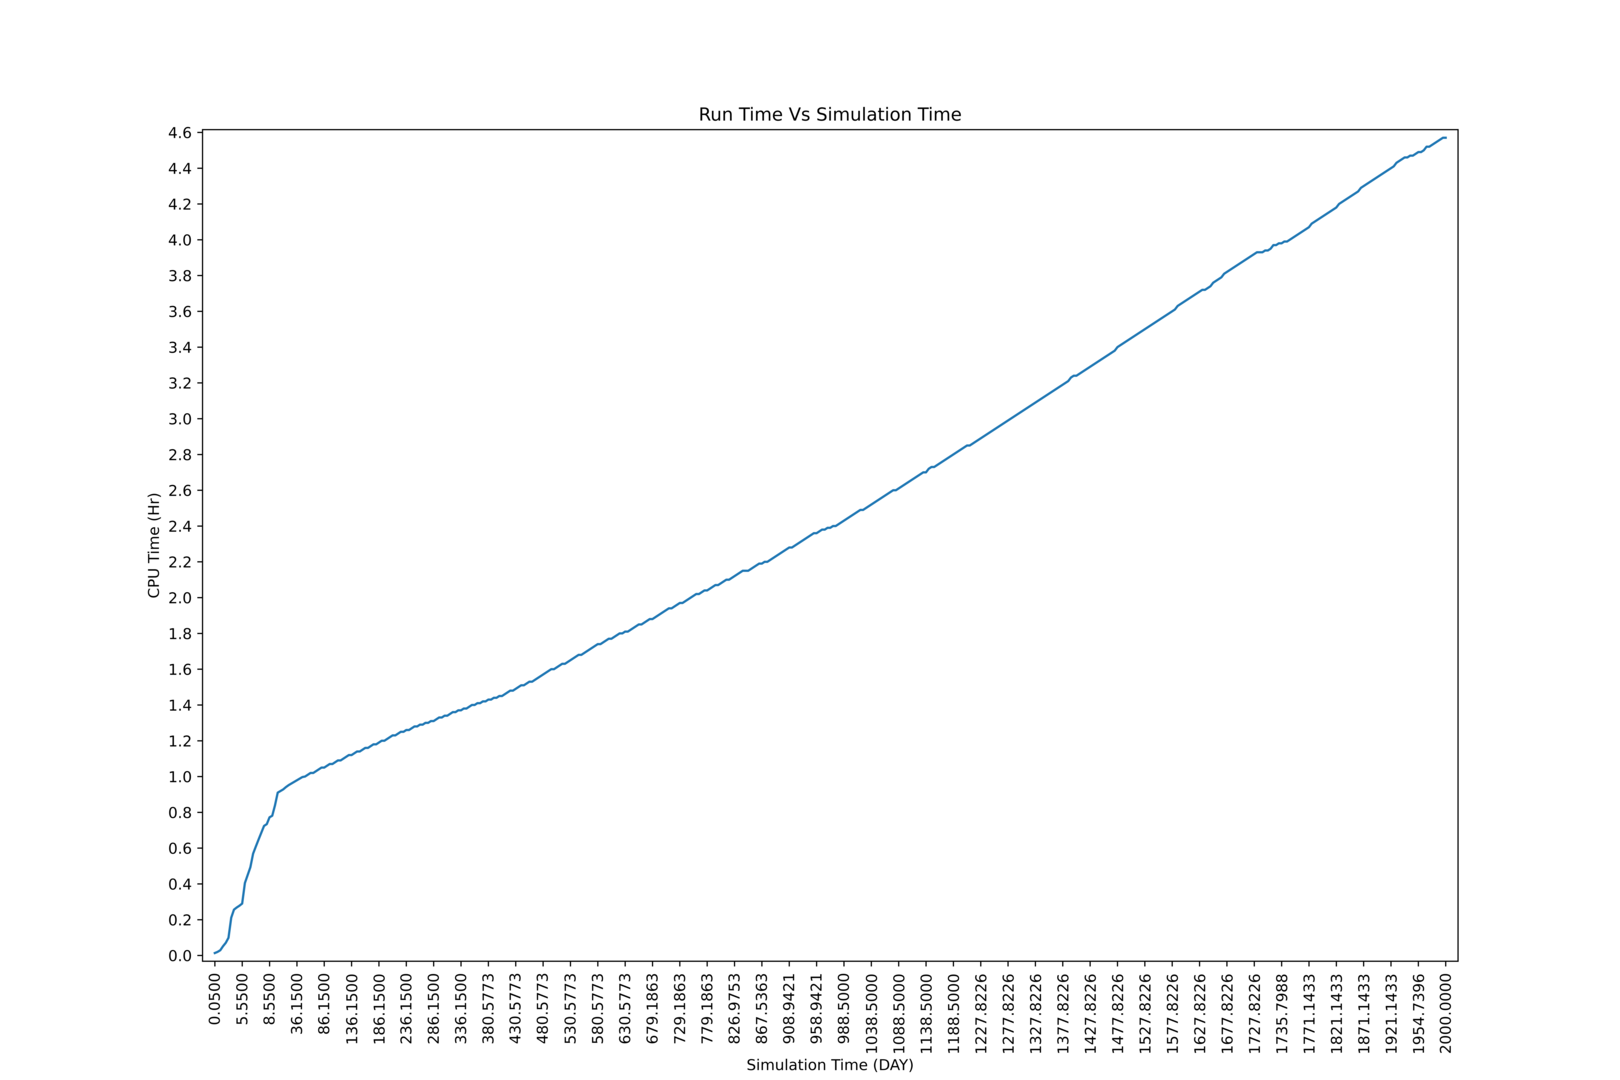
\includegraphics[width=1.1\linewidth]{figures/case3/cpr/cpu_time.png_reduced.png}
  \caption{\texttt{CPR-AMG} preconditioner.}
	\label{case3_cpu_cpr}
\end{subfigure}%
\begin{subfigure}{.5\textwidth}
  \centering
  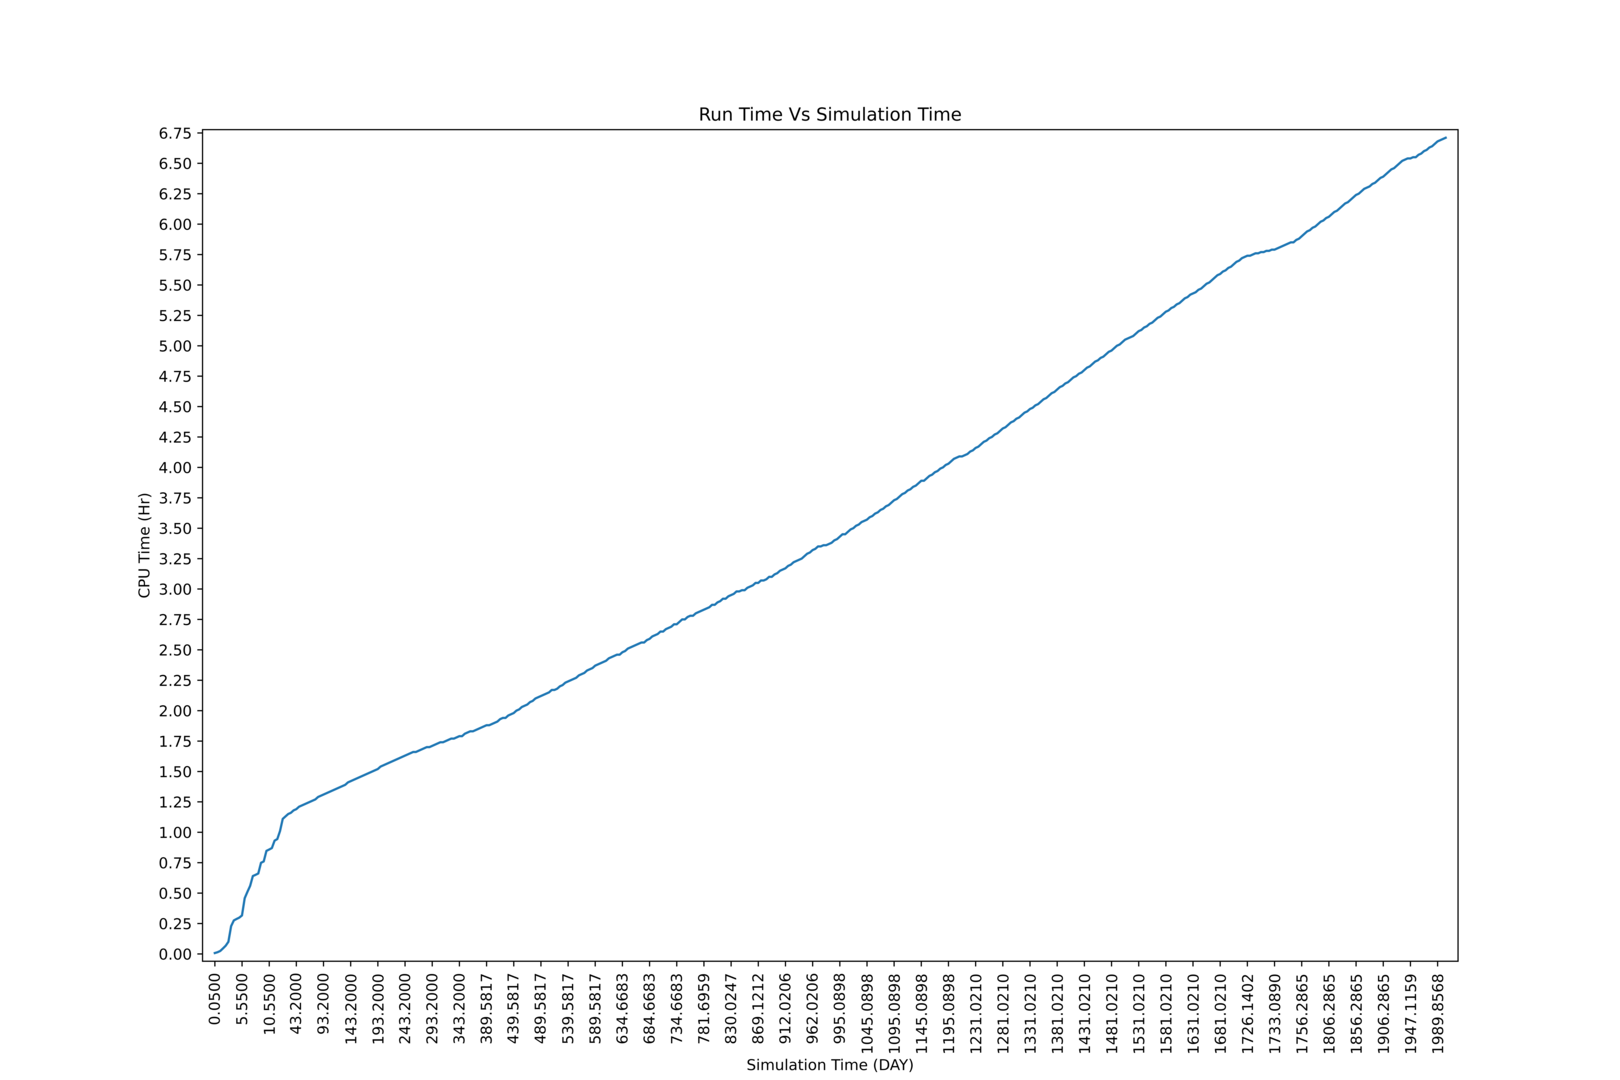
\includegraphics[width=1.1\linewidth]{figures/case3/ilu/cpu_time.png_reduced.png}
  \caption{\texttt{GMRES-ILU(0)} preconditioner}
	\label{case3_cpu_ilu}
\end{subfigure}
\begin{subfigure}{.5\textwidth}
  \centering
  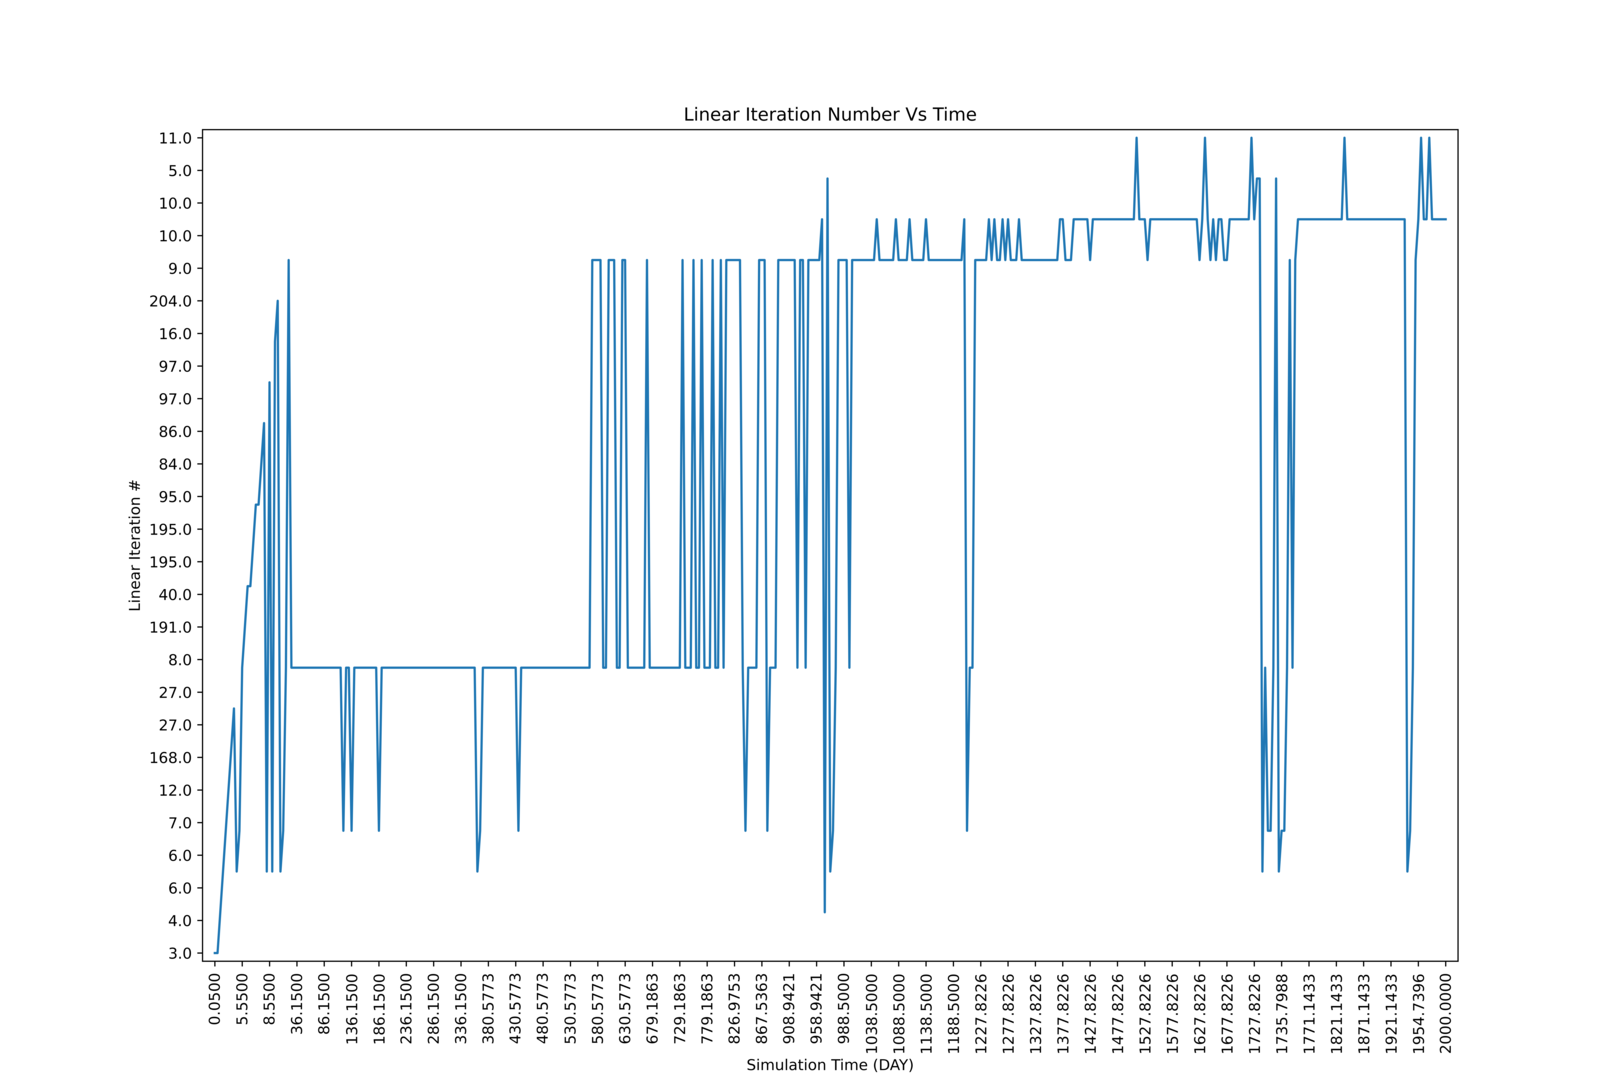
\includegraphics[width=1.1\linewidth]{figures/case3/cpr/its_time.png_reduced.png}
  \caption{\texttt{CPR-AMG} preconditioner.}
	\label{case3_its_cpr}
\end{subfigure}%
\begin{subfigure}{.5\textwidth}
  \centering
  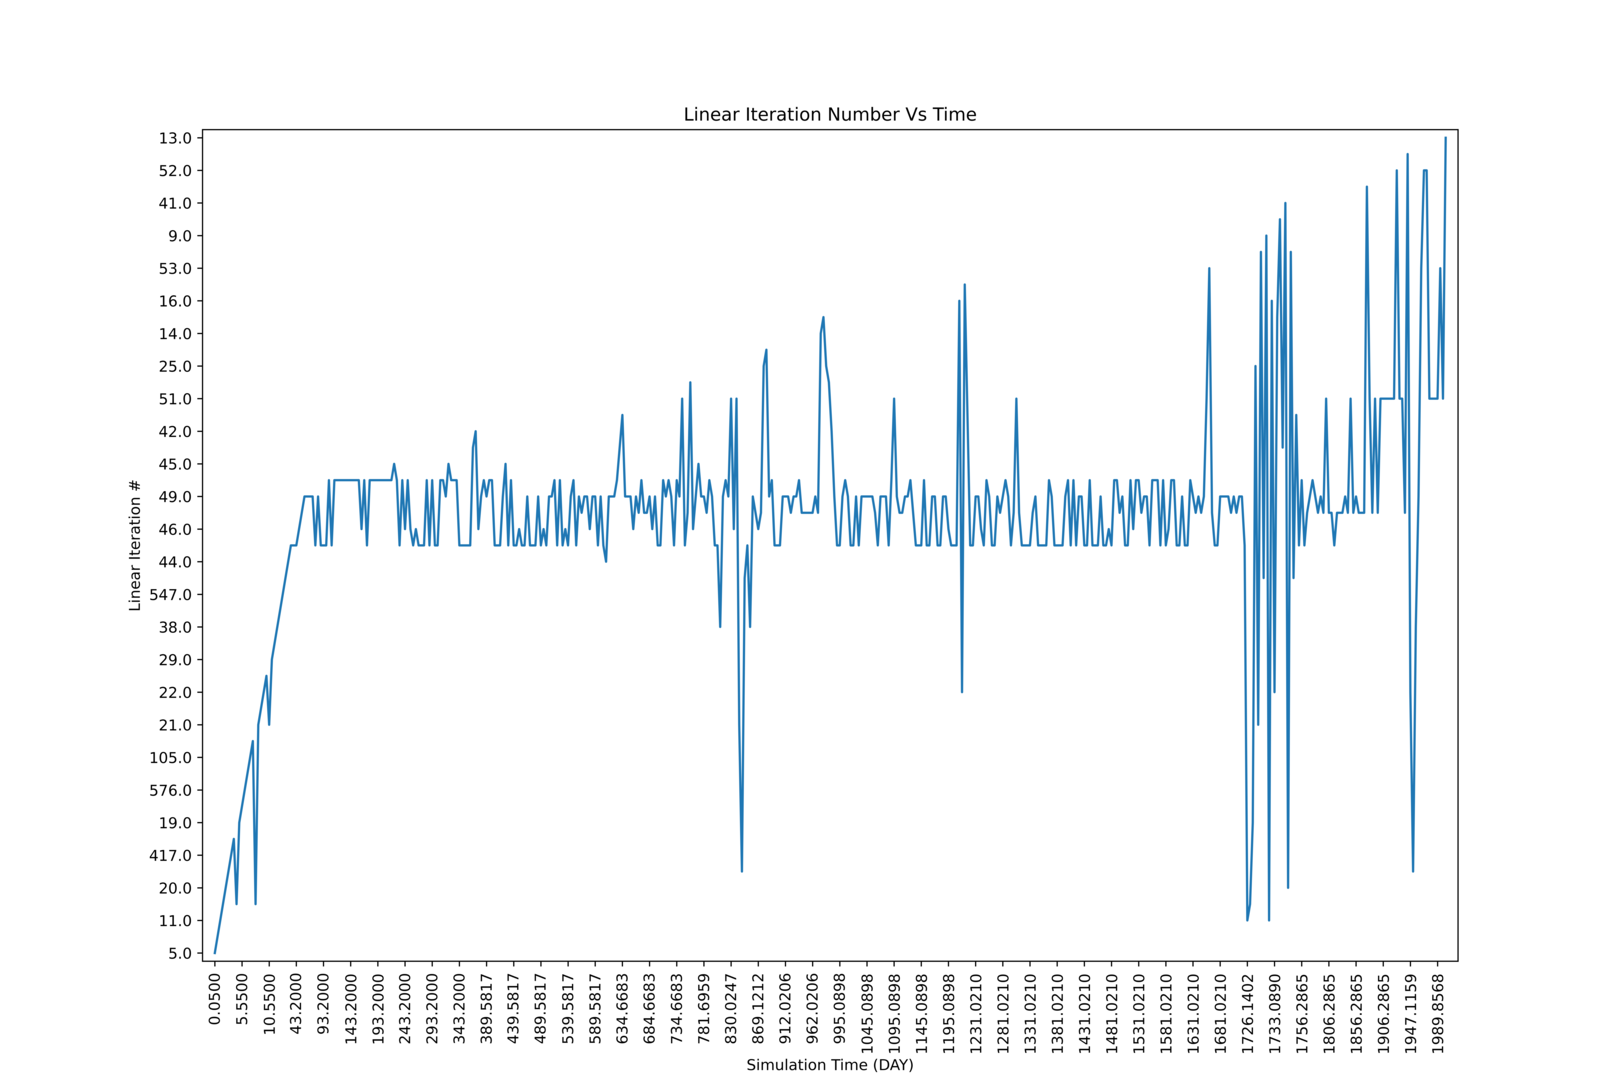
\includegraphics[width=1.1\linewidth]{figures/case3/ilu/its_time.png_reduced.png}
  \caption{\texttt{GMRES-ILU(0)} preconditioner}
	\label{case3_its_ilu}
\end{subfigure}
\begin{subfigure}{.5\textwidth}
  \centering
  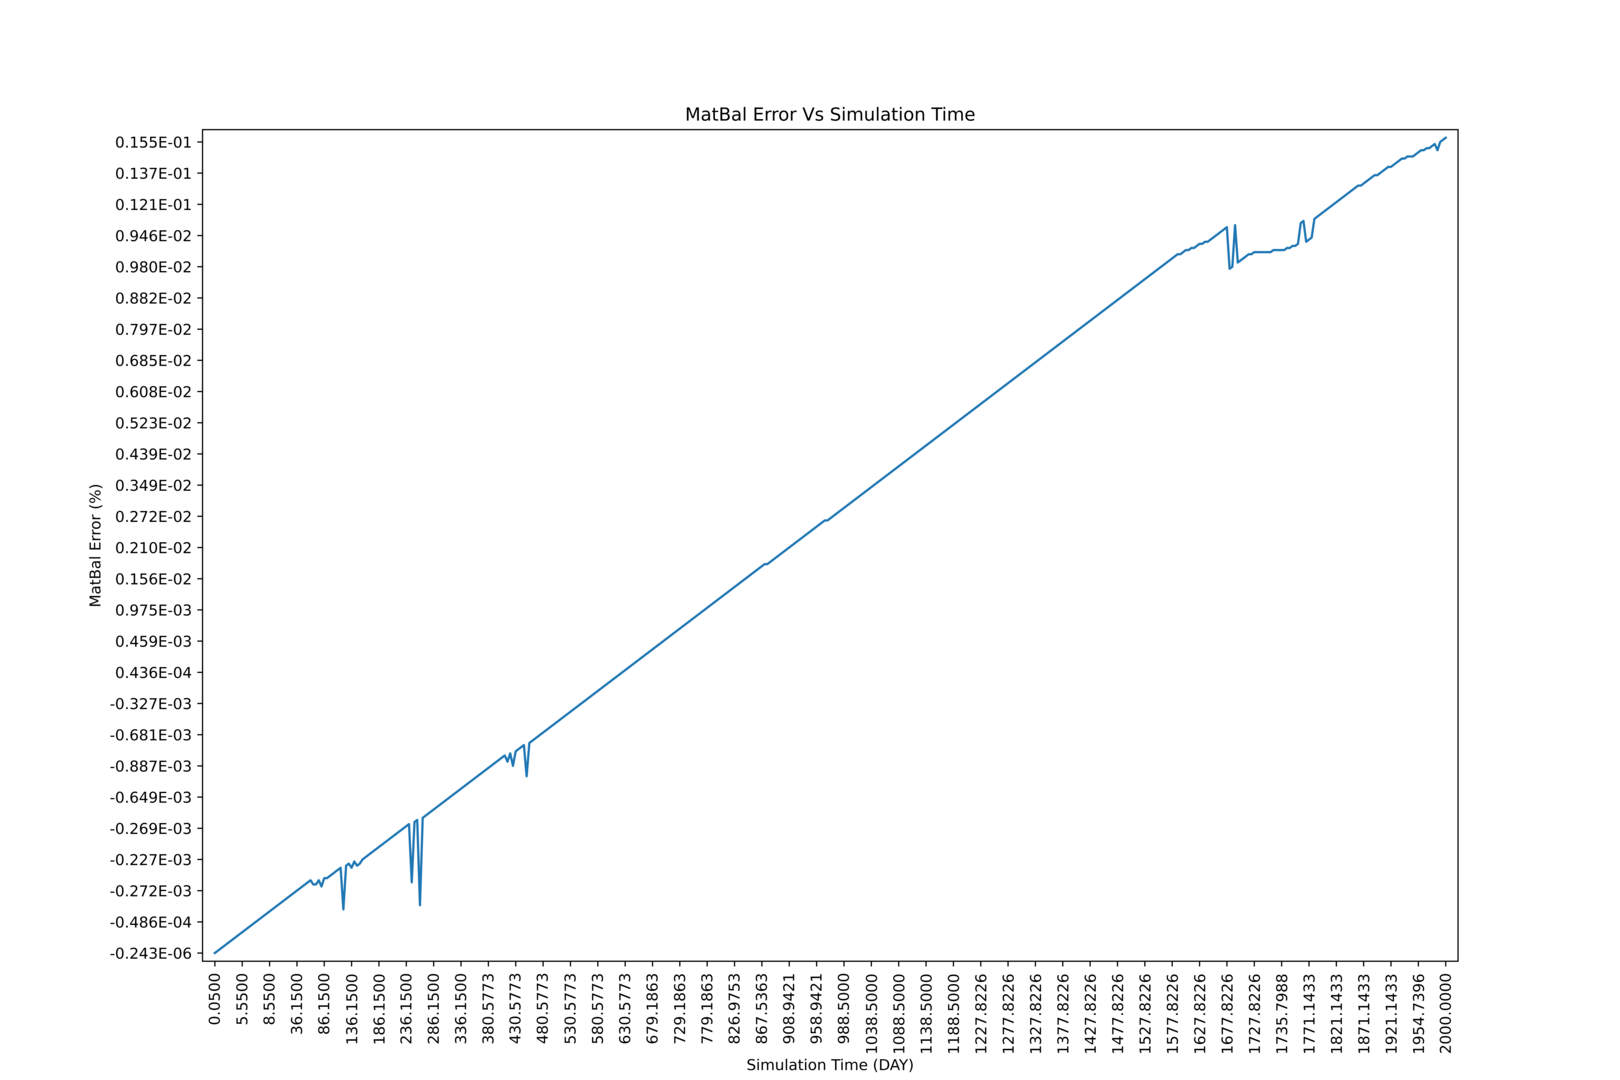
\includegraphics[width=1.1\linewidth]{figures/case3/cpr/matbalerr_time.png_reduced.png}
  \caption{\texttt{CPR-AMG} preconditioner.}
	\label{case3_matbalerr_cpr}
\end{subfigure}%
\begin{subfigure}{.5\textwidth}
  \centering
  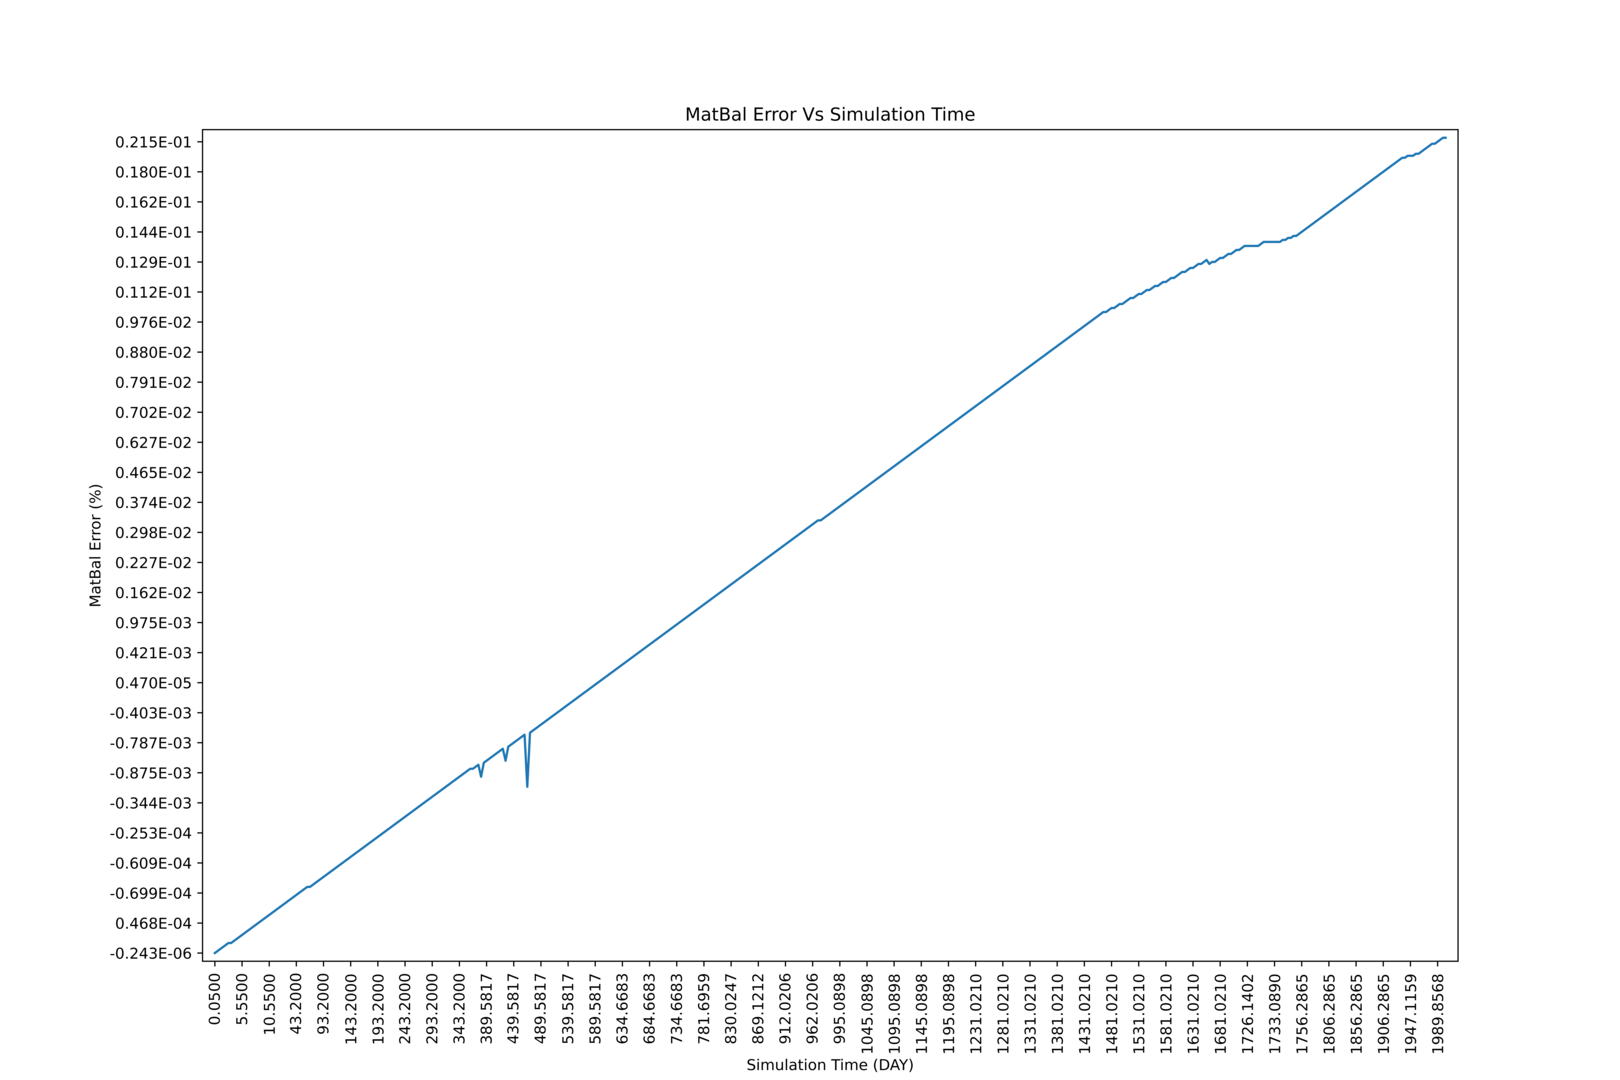
\includegraphics[width=1.1\linewidth]{figures/case3/ilu/matbalerr_time.png_reduced.png}
  \caption{\texttt{GMRES-ILU(0)} preconditioner}
	\label{case3_matbalerr_ilu}
\end{subfigure}
\caption[caption]{A comparison for \texttt{Case 3} for the two different preconditioning methods.\\\hspace{\textwidth}
		\cref{case3_cpu_cpr,case3_cpu_ilu}: CPU run time against simulation time. \\\hspace{\textwidth}
		\cref{case3_its_cpr,case3_its_ilu}: Linear iterations against simulation time.\\\hspace{\textwidth}
		\cref{case3_matbalerr_cpr,case3_matbalerr_ilu}: Material balance error against simulation time.}
\label{case3sg}
\end{figure}
\clearpage

\section{Case 4}
This model simulates water flooding in a fractured reservoir. All wells are controlled by fixing bottomhole pressure.
\FloatBarrier
\begin{center}
\begin{table}[h!]
\begin{adjustbox}{width=0.7\textwidth}
    \begin{threeparttable}
    \caption{\textbf{Case 4 Reservoir Parameters\supercite{phdfernandes}.}}
    \label{case4}
        \begin{tabular}{l r }
            \toprule
            Simulatoin Parameters & Value\\
            \midrule
	\rowcolor{red!20}\textit{\textbf{Reservoir data}}      & \\
	Grid:      &           $200\times400\times25$ ($465,816$ active) \\
	\rowcolor{blue!5}Number of wells:      &  49 (25 injector / 24 producer) \\
	Length, width and thickness:      & $4,000$ ft, $8,000$ ft and $150$ ft\\
	\rowcolor{blue!5}Porosity:       &          $0.30$ \\
	Permeability ($X, \ Y, \ Z$) & $10, \ 10$ and $1$ mD\\
	\rowcolor{blue!5}Fracture permeability & $10,000$ mD\\
	Fracture aperture	& $0.01$ ft\\
	\rowcolor{blue!5}Initial water saturation:    & $0.17$ \\      
	Formation temperature:    & $86$ F$^{\circ}$     \\
	\rowcolor{blue!5}Initial pressure:    &      $3,000$ psi\\
	Reservoir’s initial composition ($C_{1}$, $C_{3}$, $C_{10}$) & $0.01$, $0.19$, $0.8$\\
        \bottomrule
        \end{tabular}
    \end{threeparttable}
\end{adjustbox}    
\end{table}
\end{center}
\FloatBarrier

\begin{table}[h!]
   \caption{Comparison parameters for \texttt{Case 4}.}
   \label{case4-tab}
   \small
   \centering
   \begin{tabular}{lcc}
   \toprule\toprule
   \textbf{Variable} & \textbf{CPR-AMG} & \textbf{GMRES-ILU(0)} \\
   \midrule
   CPU Time (hr) & 14.4 & 25.6 \\
   Solver Time (hr) & 10.3 & 21.7 \\
   \# Newton Iterations & 3,164 & 3,169 \\
   \# Solver Iterations & 9,572 & 88,872 \\
   \# Time Steps & 849 & 850 \\
   \bottomrule
   \end{tabular}
\end{table}

\begin{figure}
\centering
\begin{subfigure}{.5\textwidth}
  \centering
  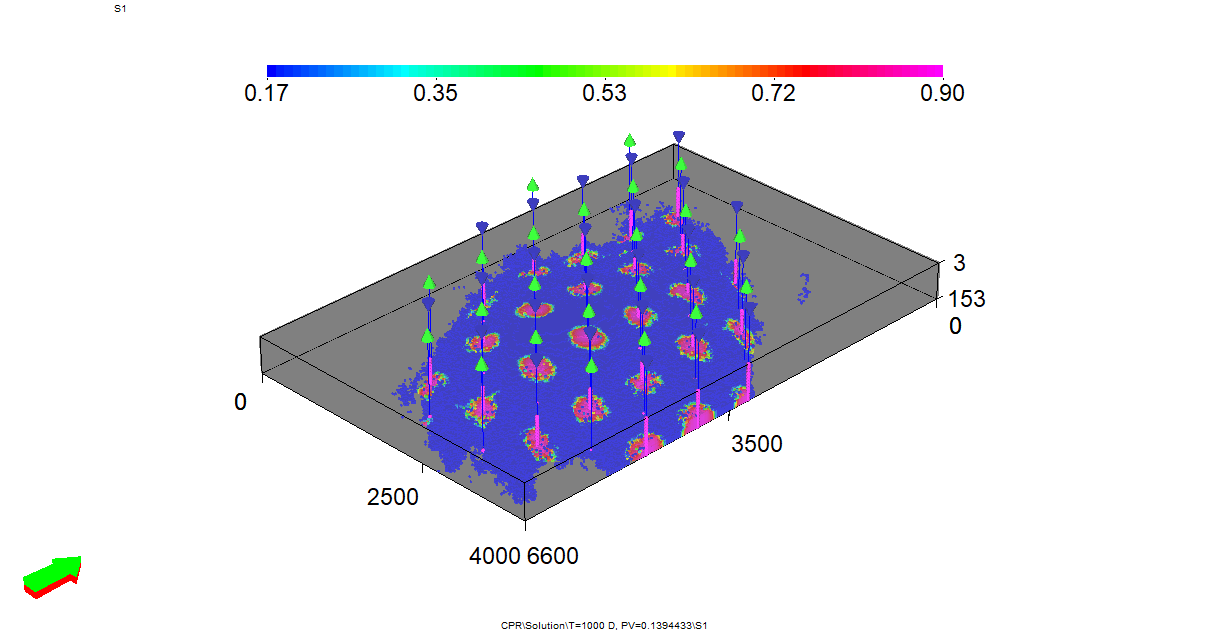
\includegraphics[width=1.3\linewidth]{figures/Case8_CPR_Sw.png}
  \caption{\texttt{CPR-AMG} preconditioner.}
\end{subfigure}%
\begin{subfigure}{.5\textwidth}
  \centering
  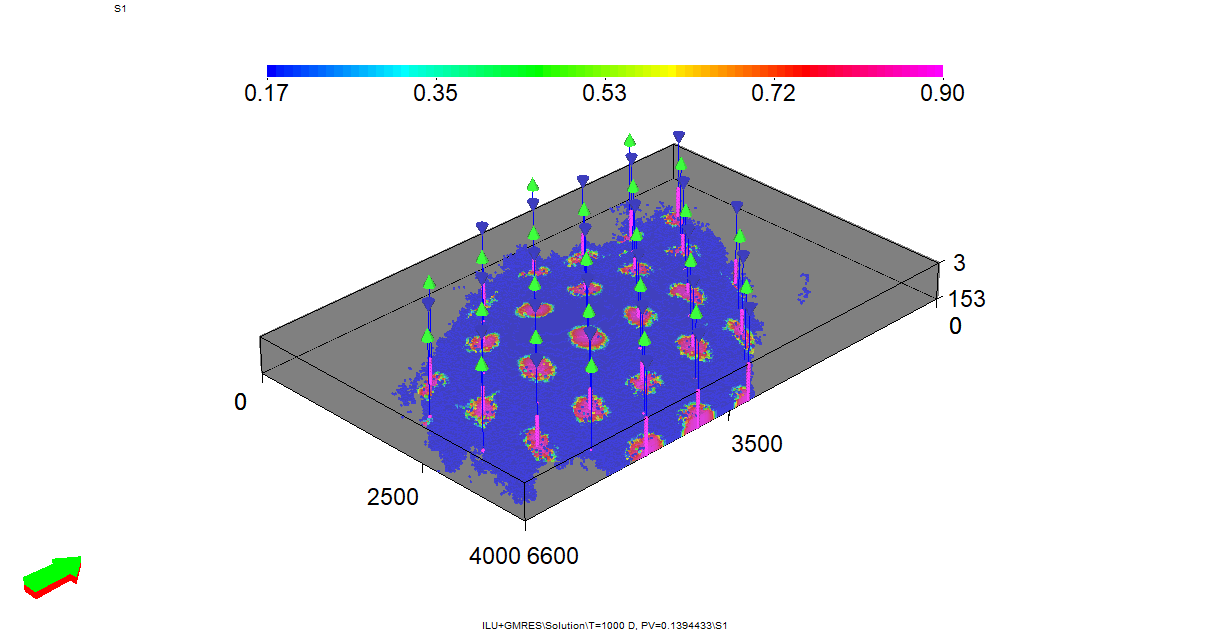
\includegraphics[width=1.3\linewidth]{figures/Case8_ILU-GMRES_Sw.png}
  \caption{\texttt{GMRES-ILU(0)} preconditioner}
\end{subfigure}
\caption{A comparison of \texttt{Case 4} water saturation $S_{w}$ distribution for the two different preconditioning methods after 1000days of simulation.}
\label{case4sw}
\end{figure}

\begin{figure}
\centering
\begin{subfigure}{.5\textwidth}
  \centering
  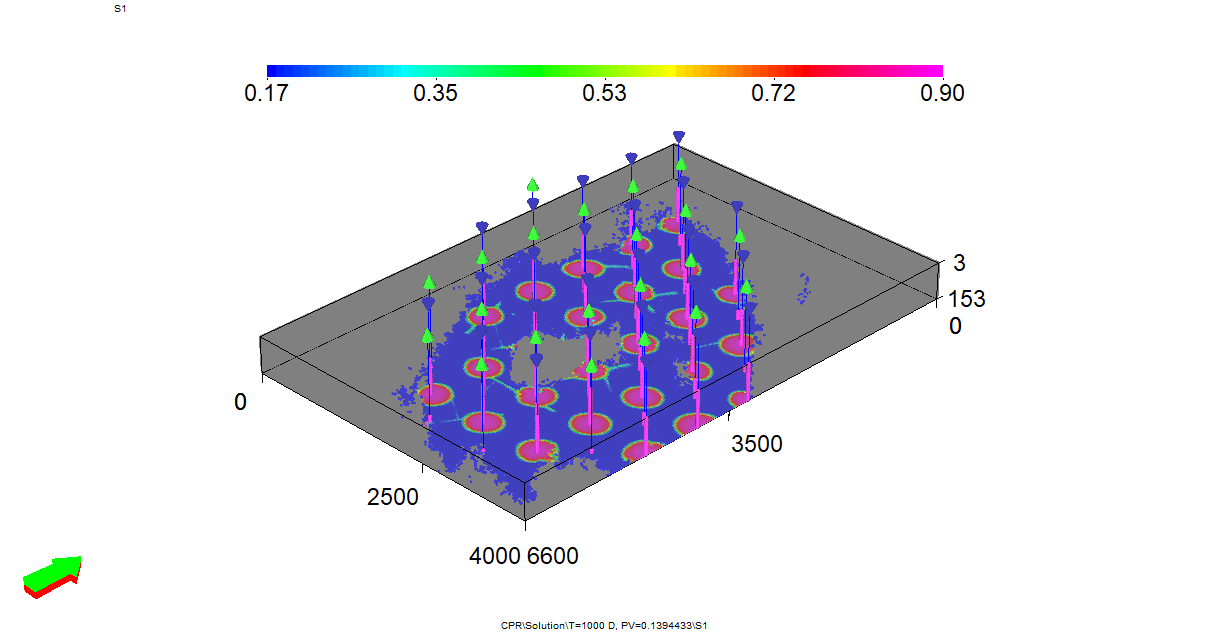
\includegraphics[width=1.3\linewidth]{figures/Case8_CPR_Sw_bl.png}
  \caption{\texttt{CPR-AMG} preconditioner.}
\end{subfigure}%
\begin{subfigure}{.5\textwidth}
  \centering
  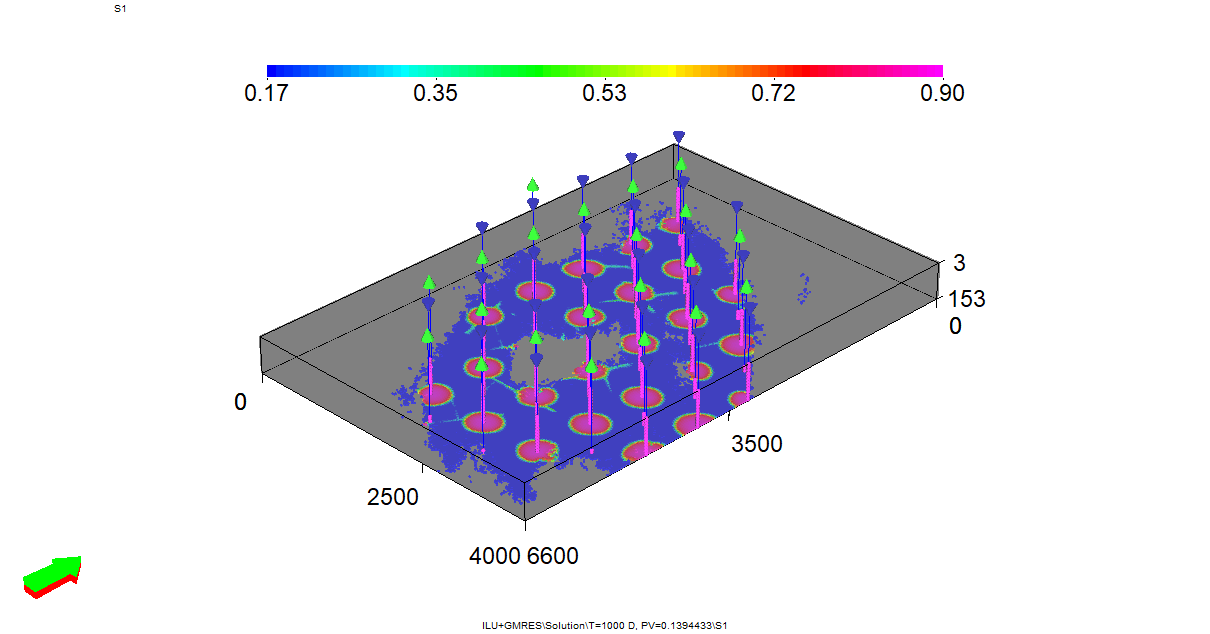
\includegraphics[width=1.3\linewidth]{figures/Case8_ILU-GMRES_Sw_bl.png}
  \caption{\texttt{GMRES-ILU(0)} preconditioner}
\end{subfigure}
\caption{A comparison of \texttt{Case 4} water saturation $S_{w}$ bottom layer for the two different preconditioning methods after 10000 days of simulation.}
\label{case4swbl}
\end{figure}

\begin{figure}
\centering
\begin{subfigure}{.5\textwidth}
  \centering
  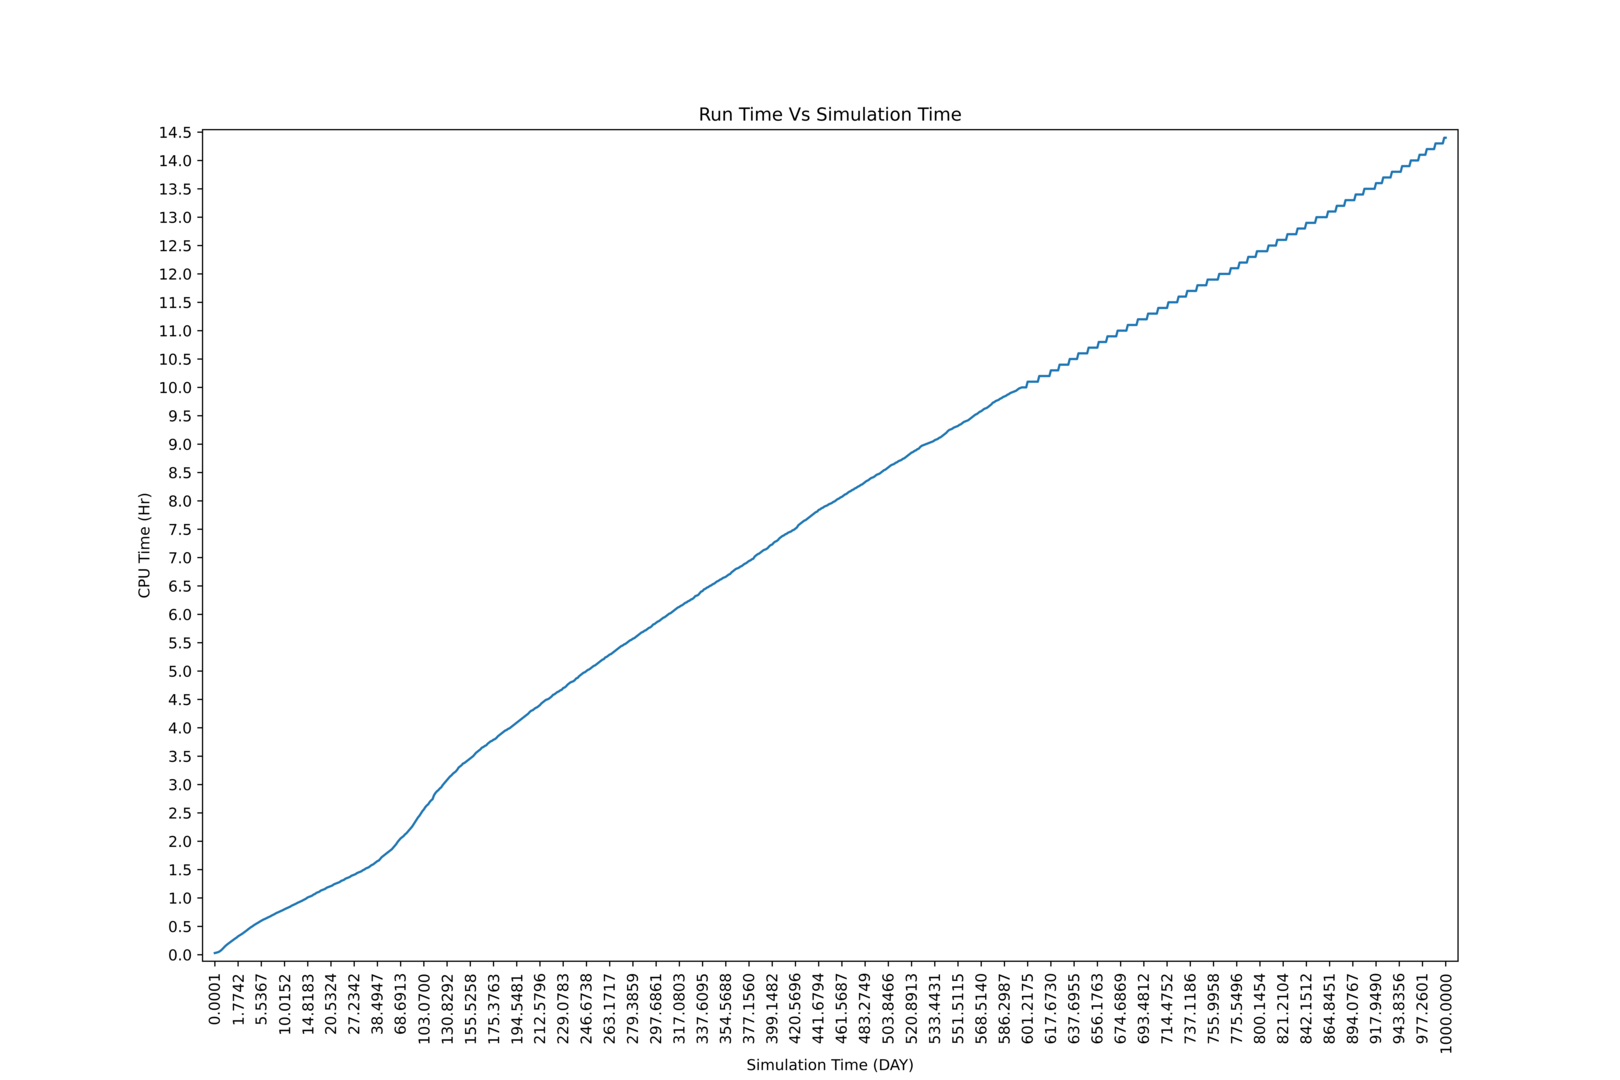
\includegraphics[width=1.1\linewidth]{figures/case8/cpr/cpu_time.png_reduced.png}
  \caption{\texttt{CPR-AMG} preconditioner.}
	\label{case8_cpu_cpr}
\end{subfigure}%
\begin{subfigure}{.5\textwidth}
  \centering
  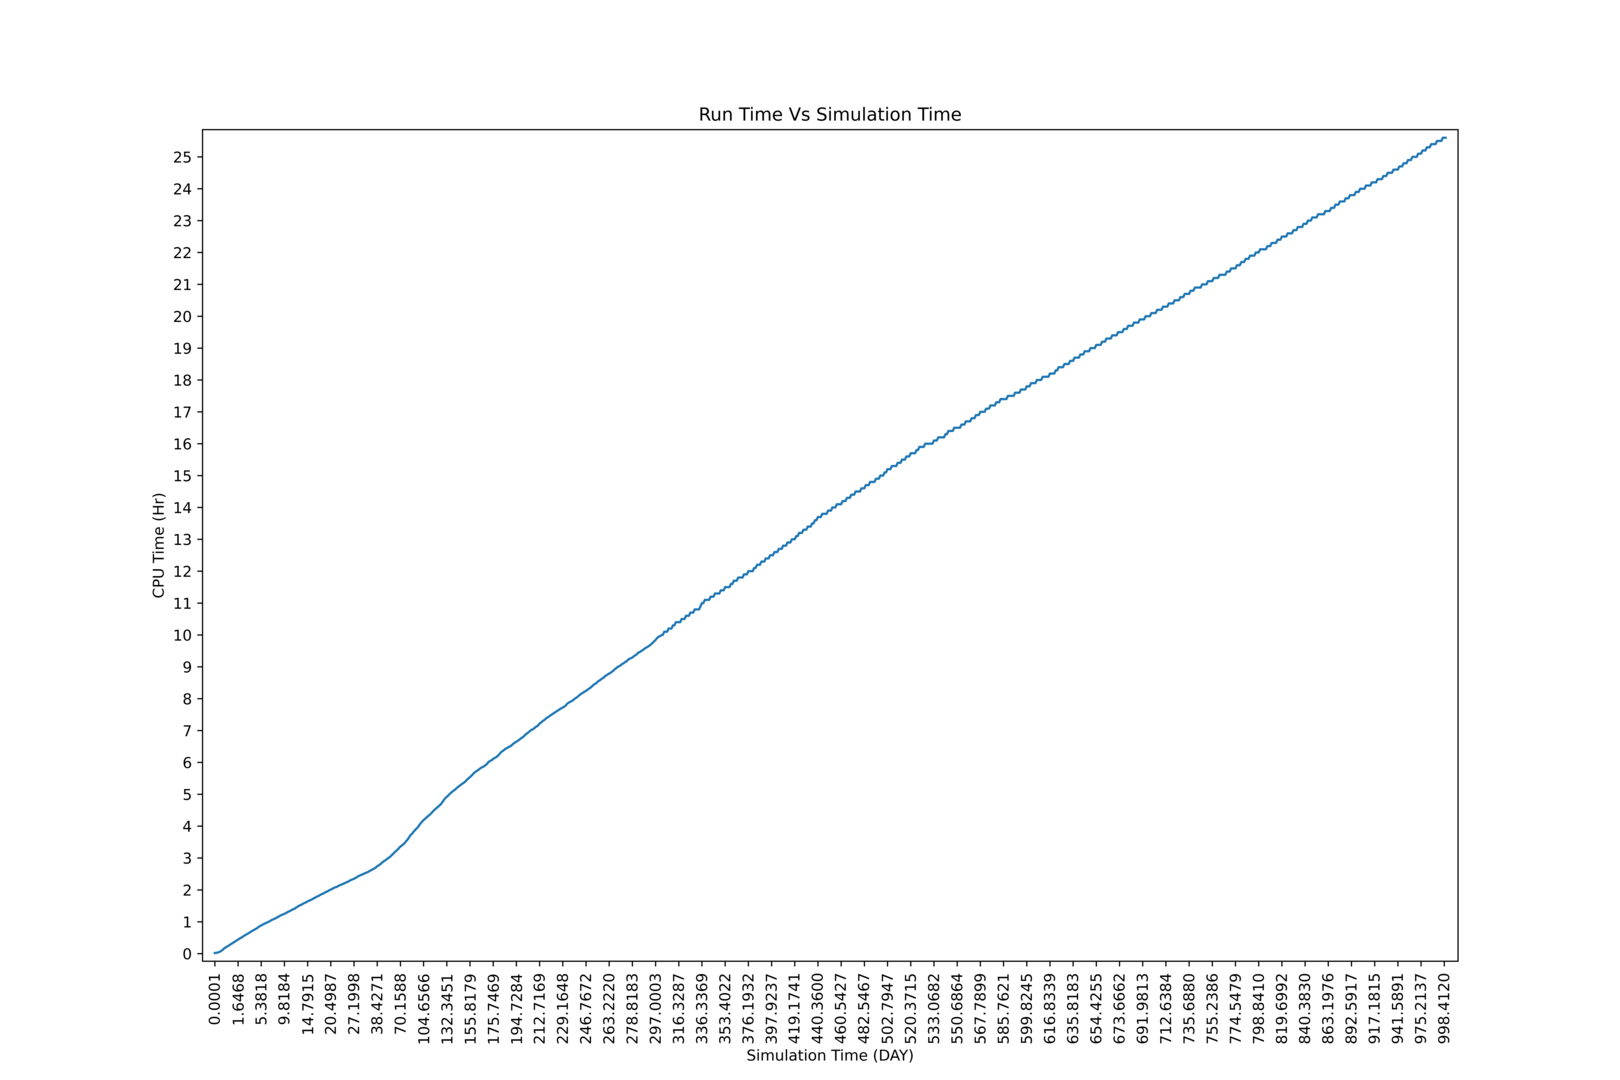
\includegraphics[width=1.1\linewidth]{figures/case8/ilu/cpu_time.png_reduced.png}
  \caption{\texttt{GMRES-ILU(0)} preconditioner}
	\label{case8_cpu_ilu}
\end{subfigure}
\begin{subfigure}{.5\textwidth}
  \centering
  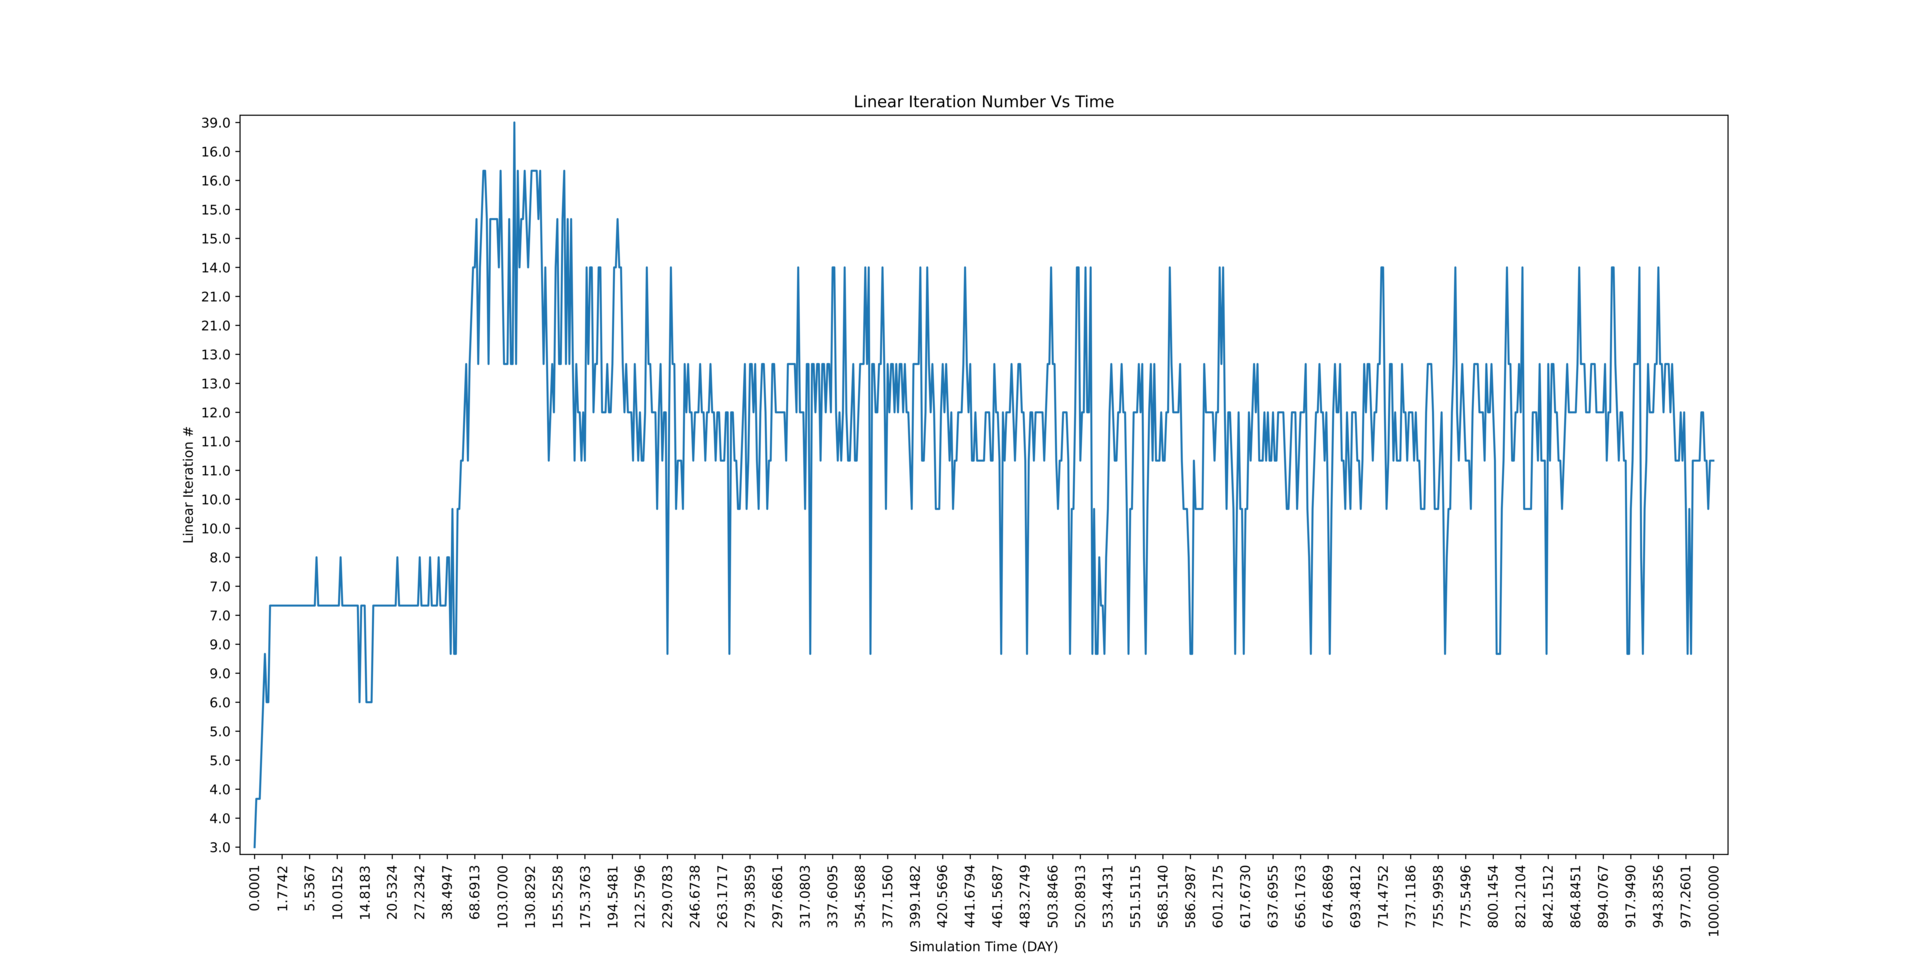
\includegraphics[width=1.1\linewidth]{figures/case8/cpr/its_time.png_reduced.png}
  \caption{\texttt{CPR-AMG} preconditioner.}
	\label{case8_its_cpr}
\end{subfigure}%
\begin{subfigure}{.5\textwidth}
  \centering
  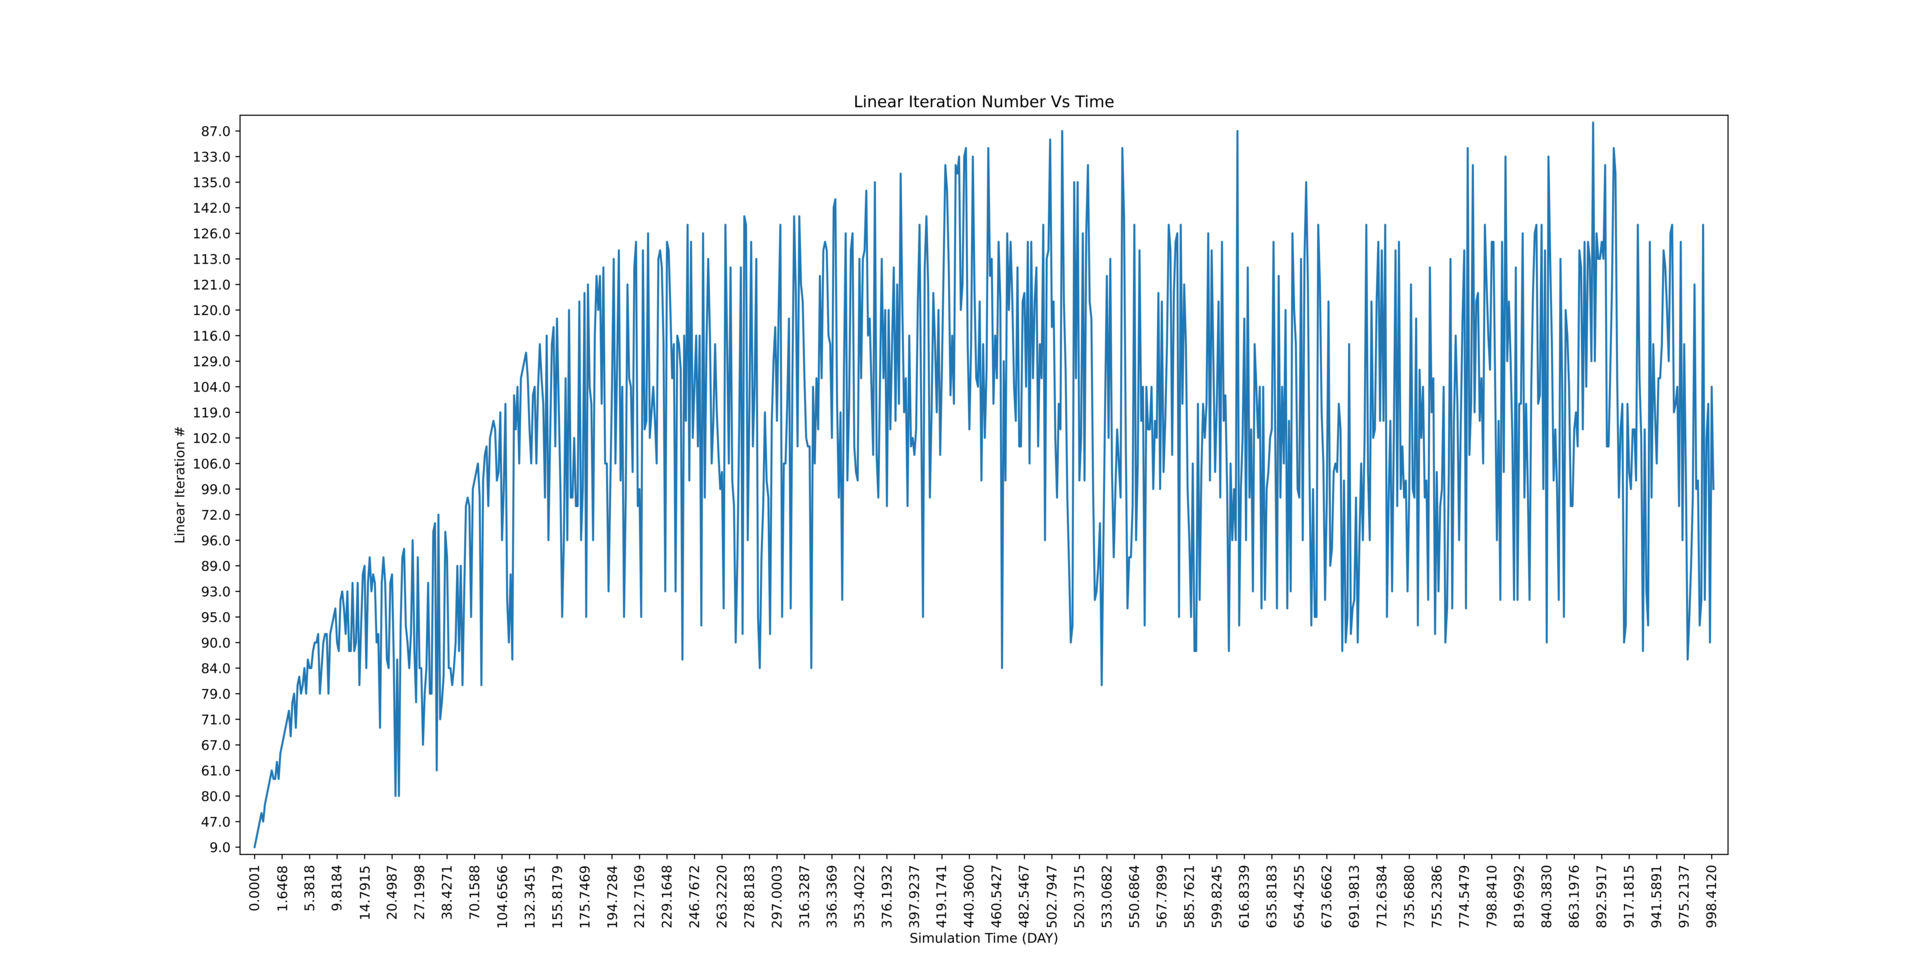
\includegraphics[width=1.1\linewidth]{figures/case8/ilu/its_time.png_reduced.png}
  \caption{\texttt{GMRES-ILU(0)} preconditioner}
	\label{case8_its_ilu}
\end{subfigure}
\begin{subfigure}{.5\textwidth}
  \centering
  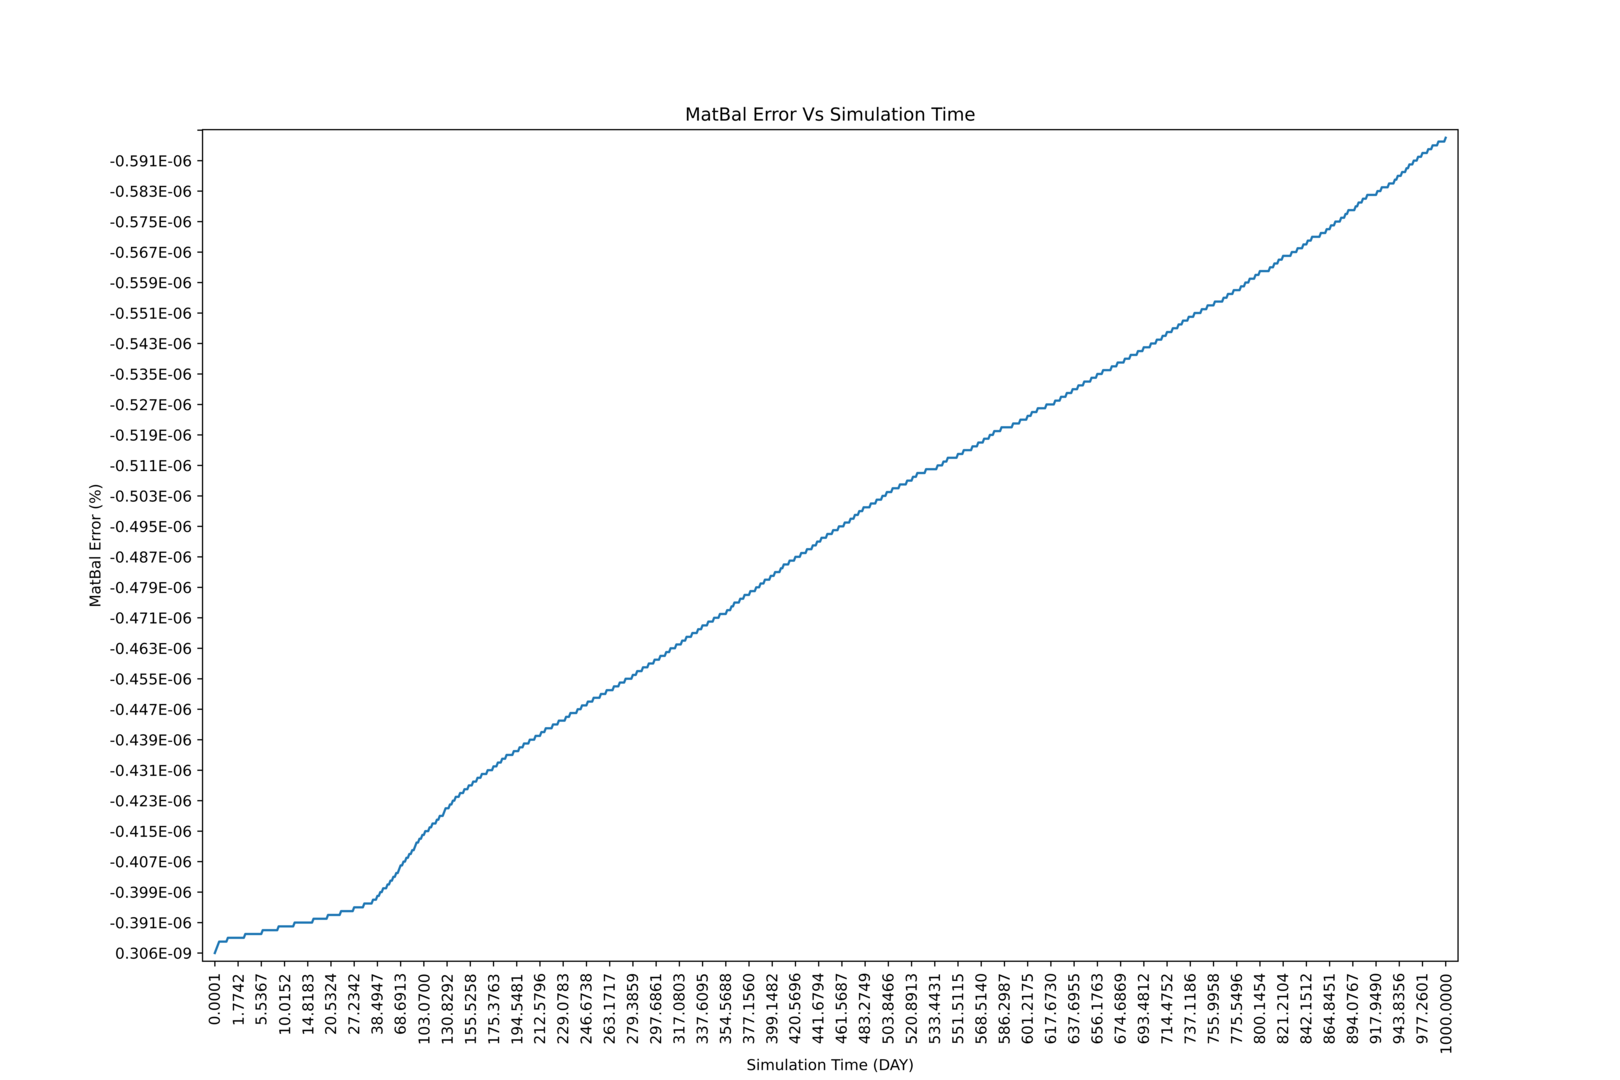
\includegraphics[width=1.1\linewidth]{figures/case8/cpr/matbalerr_time.png_reduced.png}
  \caption{\texttt{CPR-AMG} preconditioner.}
	\label{case8_matbalerr_cpr}
\end{subfigure}%
\begin{subfigure}{.5\textwidth}
  \centering
  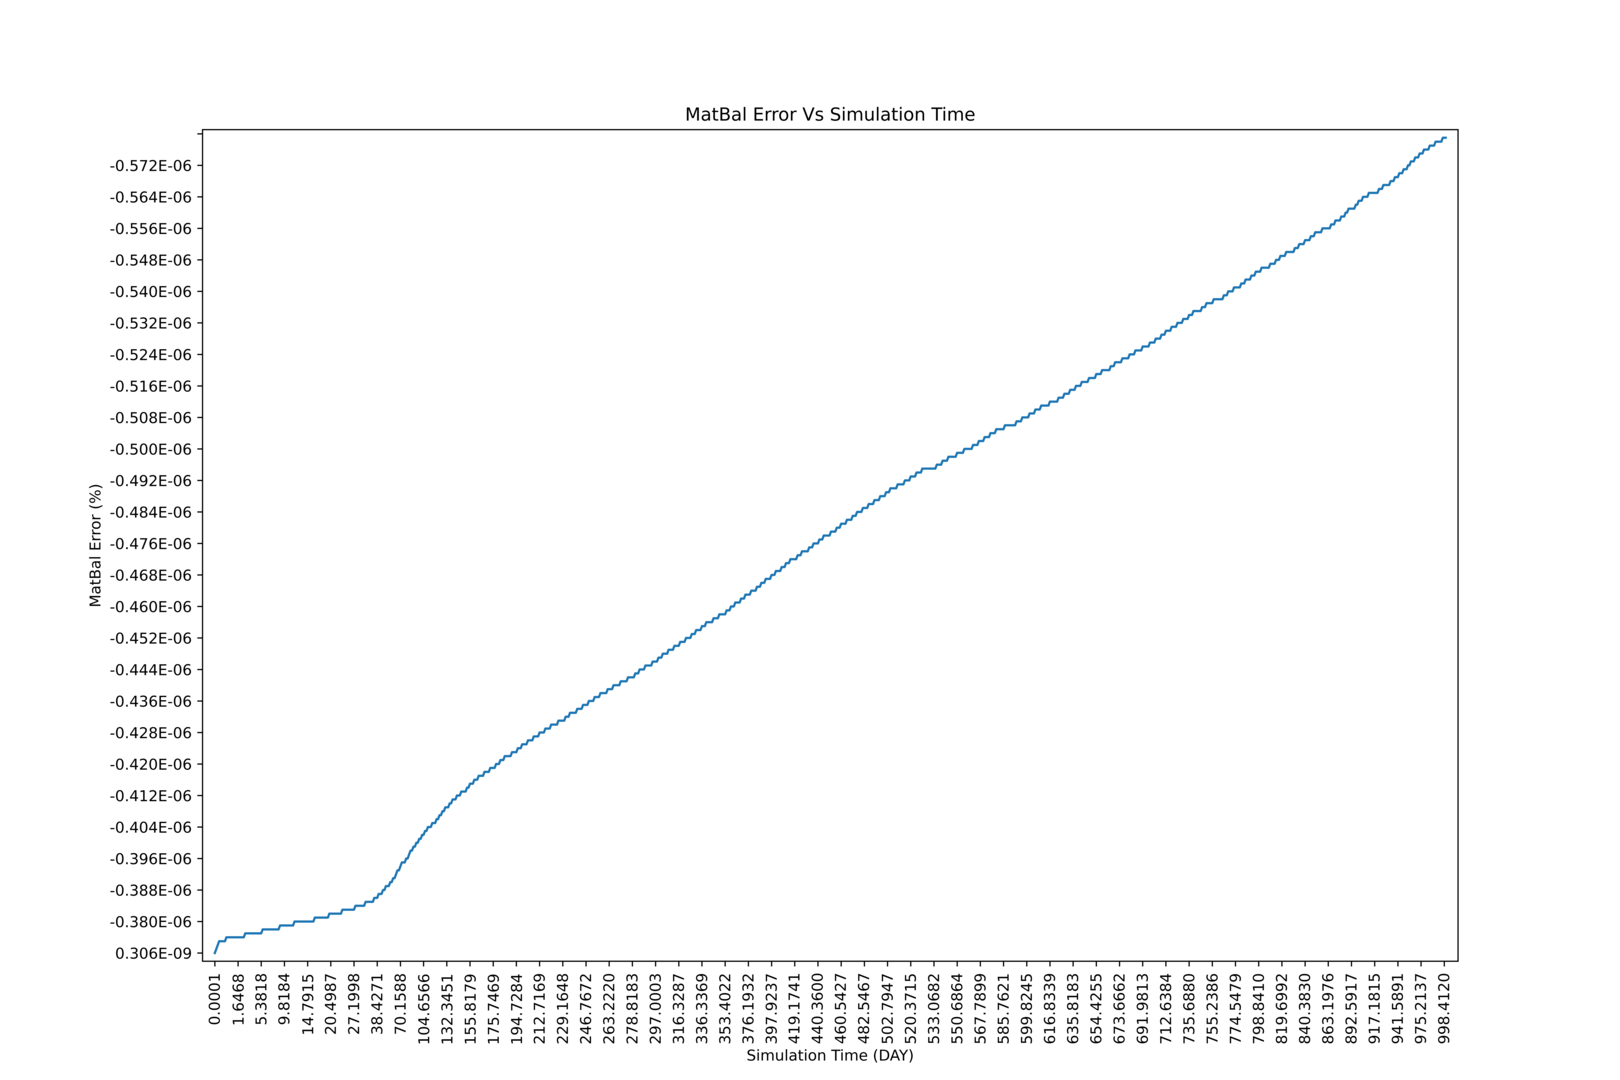
\includegraphics[width=1.1\linewidth]{figures/case8/ilu/matbalerr_time.png_reduced.png}
  \caption{\texttt{GMRES-ILU(0)} preconditioner}
	\label{case8_matbalerr_ilu}
\end{subfigure}
\caption[caption]{A comparison for \texttt{Case 4} for the two different preconditioning methods.\\\hspace{\textwidth}
		\cref{case8_cpu_cpr,case8_cpu_ilu}: CPU run time against simulation time. \\\hspace{\textwidth}
		\cref{case8_its_cpr,case8_its_ilu}: Linear iterations against simulation time.\\\hspace{\textwidth}
		\cref{case8_matbalerr_cpr,case8_matbalerr_ilu}: Material balance error against simulation time.}
\label{case8sg}
\end{figure}
\clearpage

\section{Case 5}
This model is simillar to the previous case instead of flooding with water, gas is used instead. Parameters of the reservoir
are the same as the previous case \ref{case4}.

\begin{table}[h!]
   \caption{Comparison parameters for \texttt{Case 5}.}
   \label{case5-tab}
   \small
   \centering
   \begin{tabular}{lcc}
   \toprule\toprule
   \textbf{Variable} & \textbf{CPR-AMG} & \textbf{GMRES-ILU(0)} \\
   \midrule
   CPU Time (hr) & 64.25 &  71.9 \\
   Solver Time (hr) & 49 & 56.9 \\
   \# Newton Iterations & 11,104 & 11,029 \\
   \# Solver Iterations & 92,218 & 376,594 \\
   \# Time Steps & 4,740 & 4,735 \\
   \bottomrule
   \end{tabular}
\end{table}

\begin{figure}[h!]
\centering
\begin{subfigure}{.5\textwidth}
  \centering
  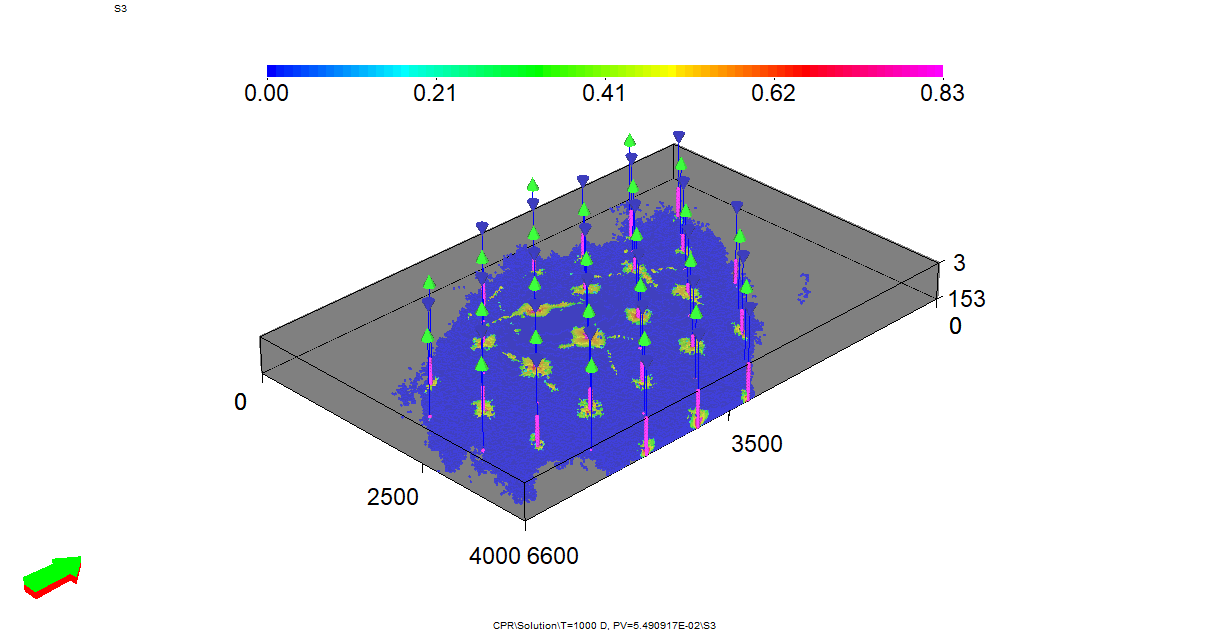
\includegraphics[width=1.3\linewidth]{figures/Case9_CPR_Sg.png}
  \caption{\texttt{CPR-AMG} preconditioner.}
\end{subfigure}%
\begin{subfigure}{.5\textwidth}
  \centering
  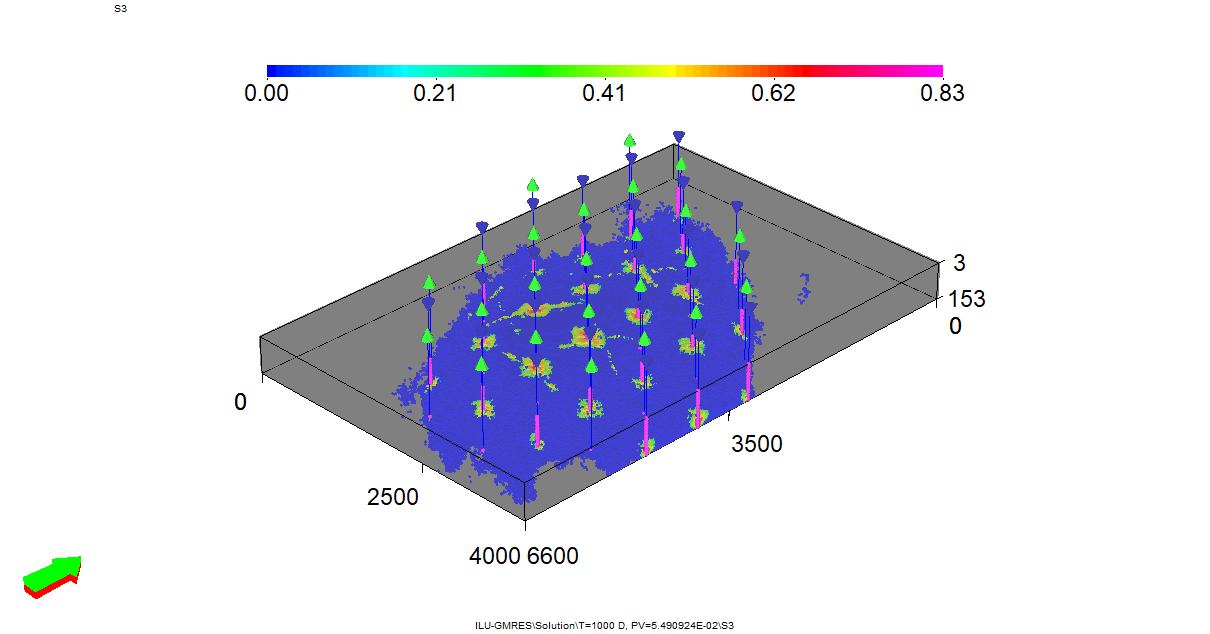
\includegraphics[width=1.3\linewidth]{figures/Case9_ILU-GMRES_Sg.png}
  \caption{\texttt{GMRES-ILU(0)} preconditioner}
\end{subfigure}
\caption{A comparison of \texttt{Case 5} gas saturation $S_{g}$ distribution for the two different preconditioning methods after 1000days of simulation.}
\label{case5sg}
\end{figure}

\begin{figure}
\centering
\begin{subfigure}{.5\textwidth}
  \centering
  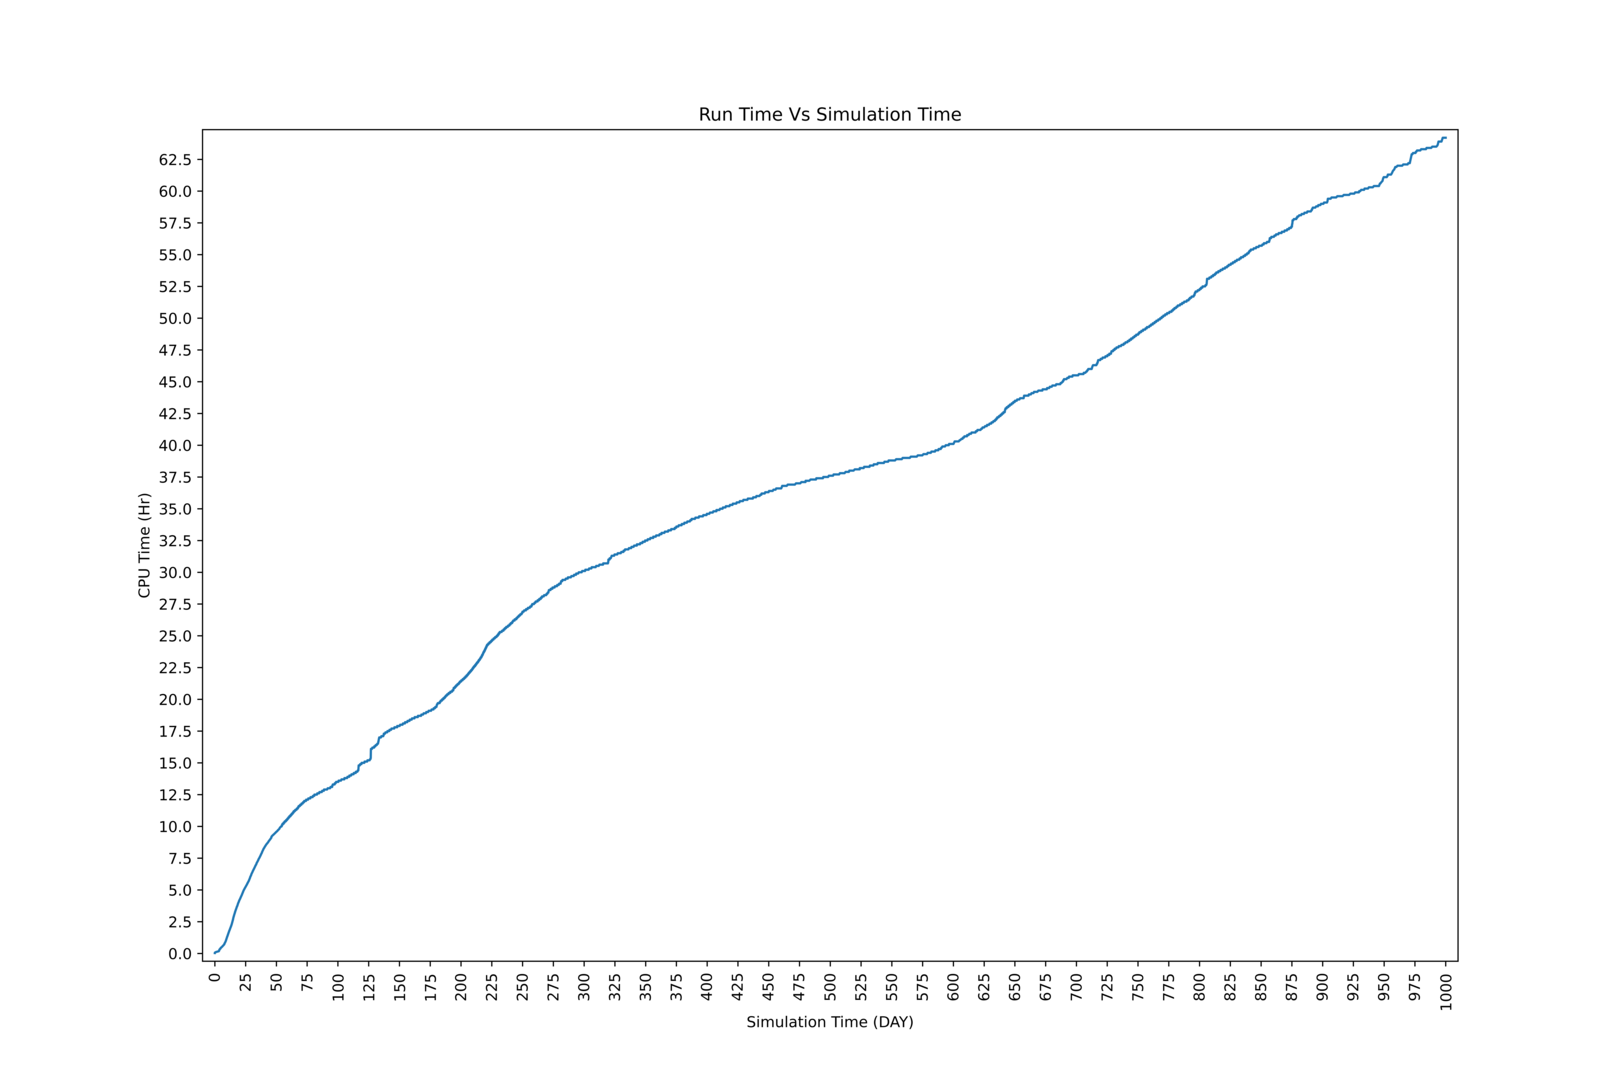
\includegraphics[width=1.1\linewidth]{figures/case9/cpr/cpu_time.png_reduced.png}
  \caption{\texttt{CPR-AMG} preconditioner.}
	\label{case9_cpu_cpr}
\end{subfigure}%
\begin{subfigure}{.5\textwidth}
  \centering
  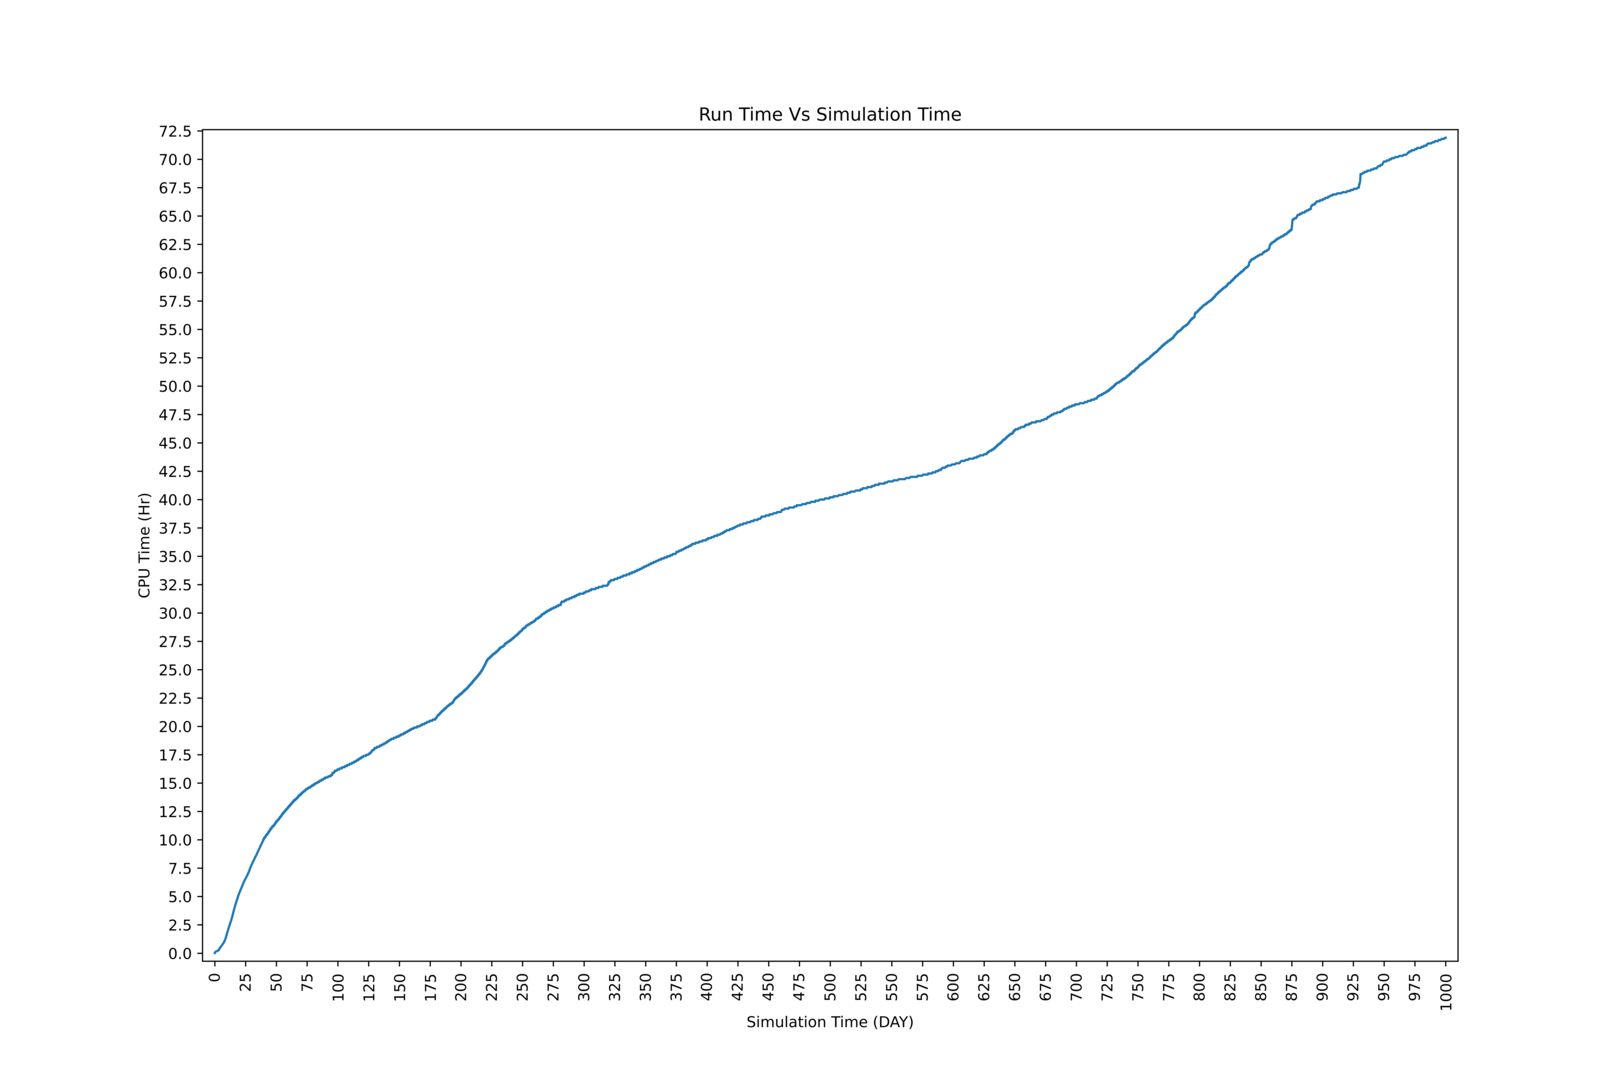
\includegraphics[width=1.1\linewidth]{figures/case9/ilu/cpu_time.png_reduced.png}
  \caption{\texttt{GMRES-ILU(0)} preconditioner}
	\label{case9_cpu_ilu}
\end{subfigure}
\begin{subfigure}{.5\textwidth}
  \centering
  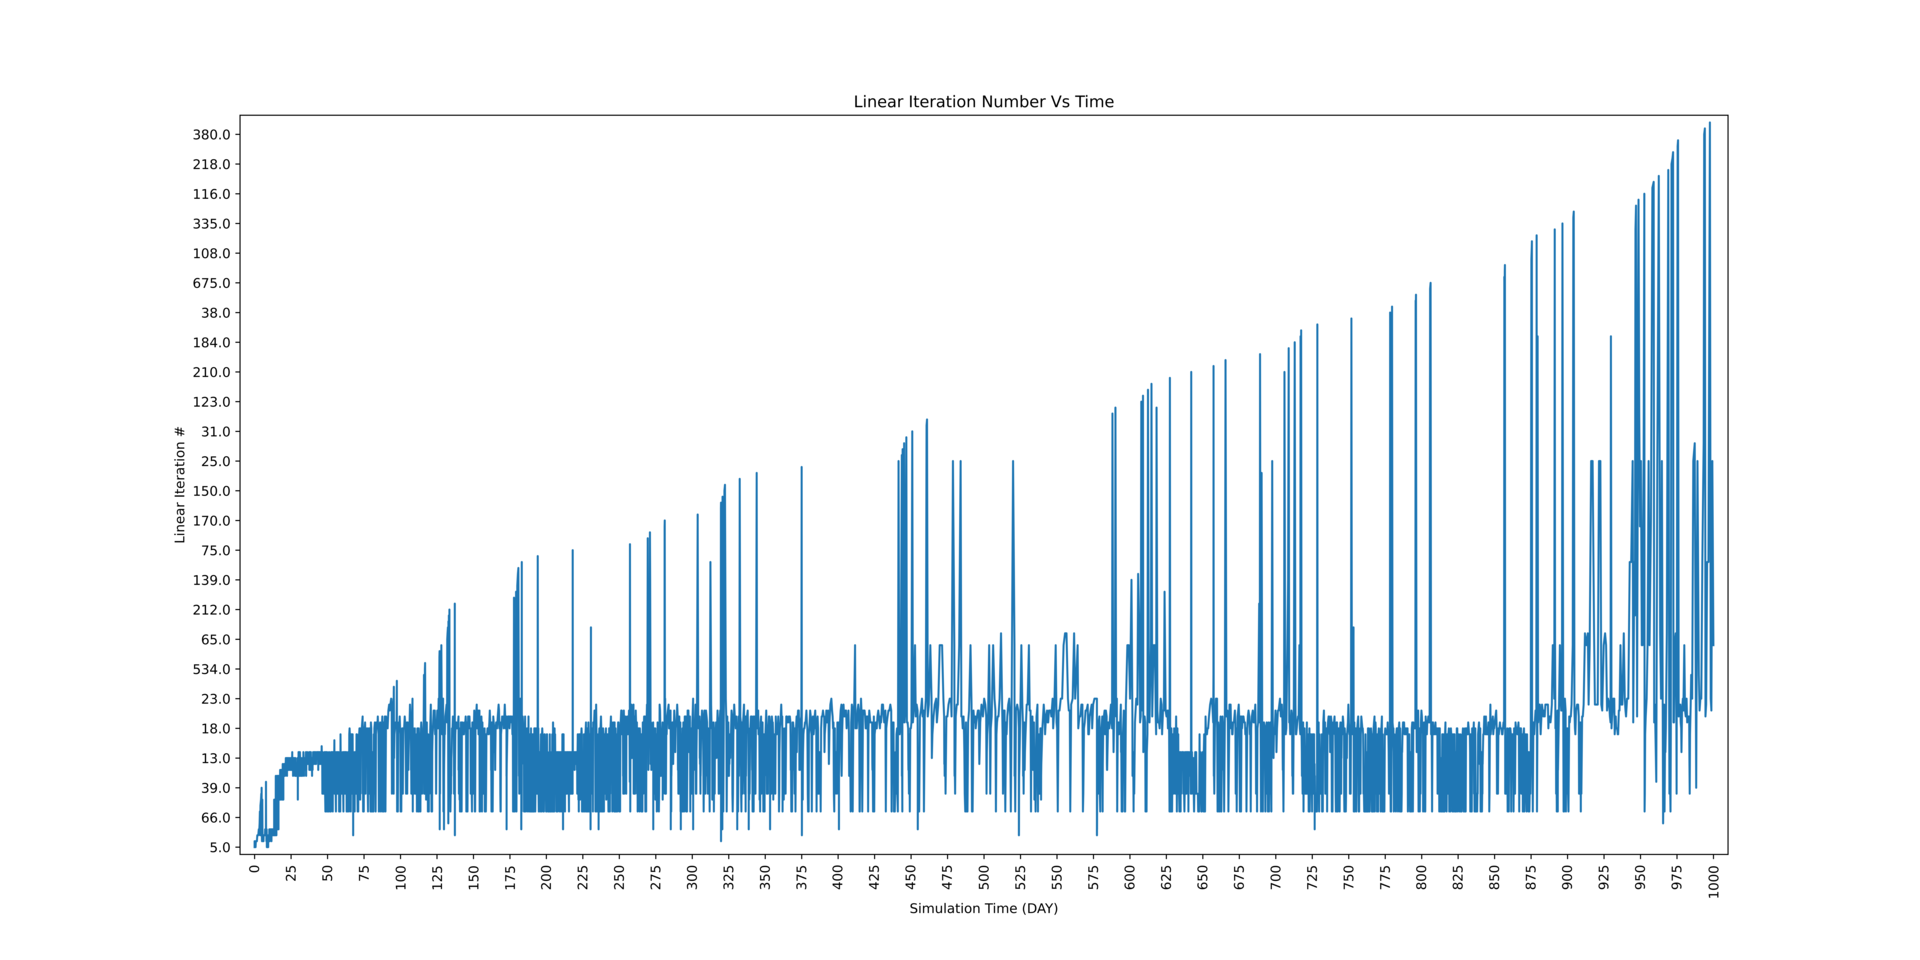
\includegraphics[width=1.1\linewidth]{figures/case9/cpr/its_time.png_reduced.png}
  \caption{\texttt{CPR-AMG} preconditioner.}
	\label{case9_its_cpr}
\end{subfigure}%
\begin{subfigure}{.5\textwidth}
  \centering
  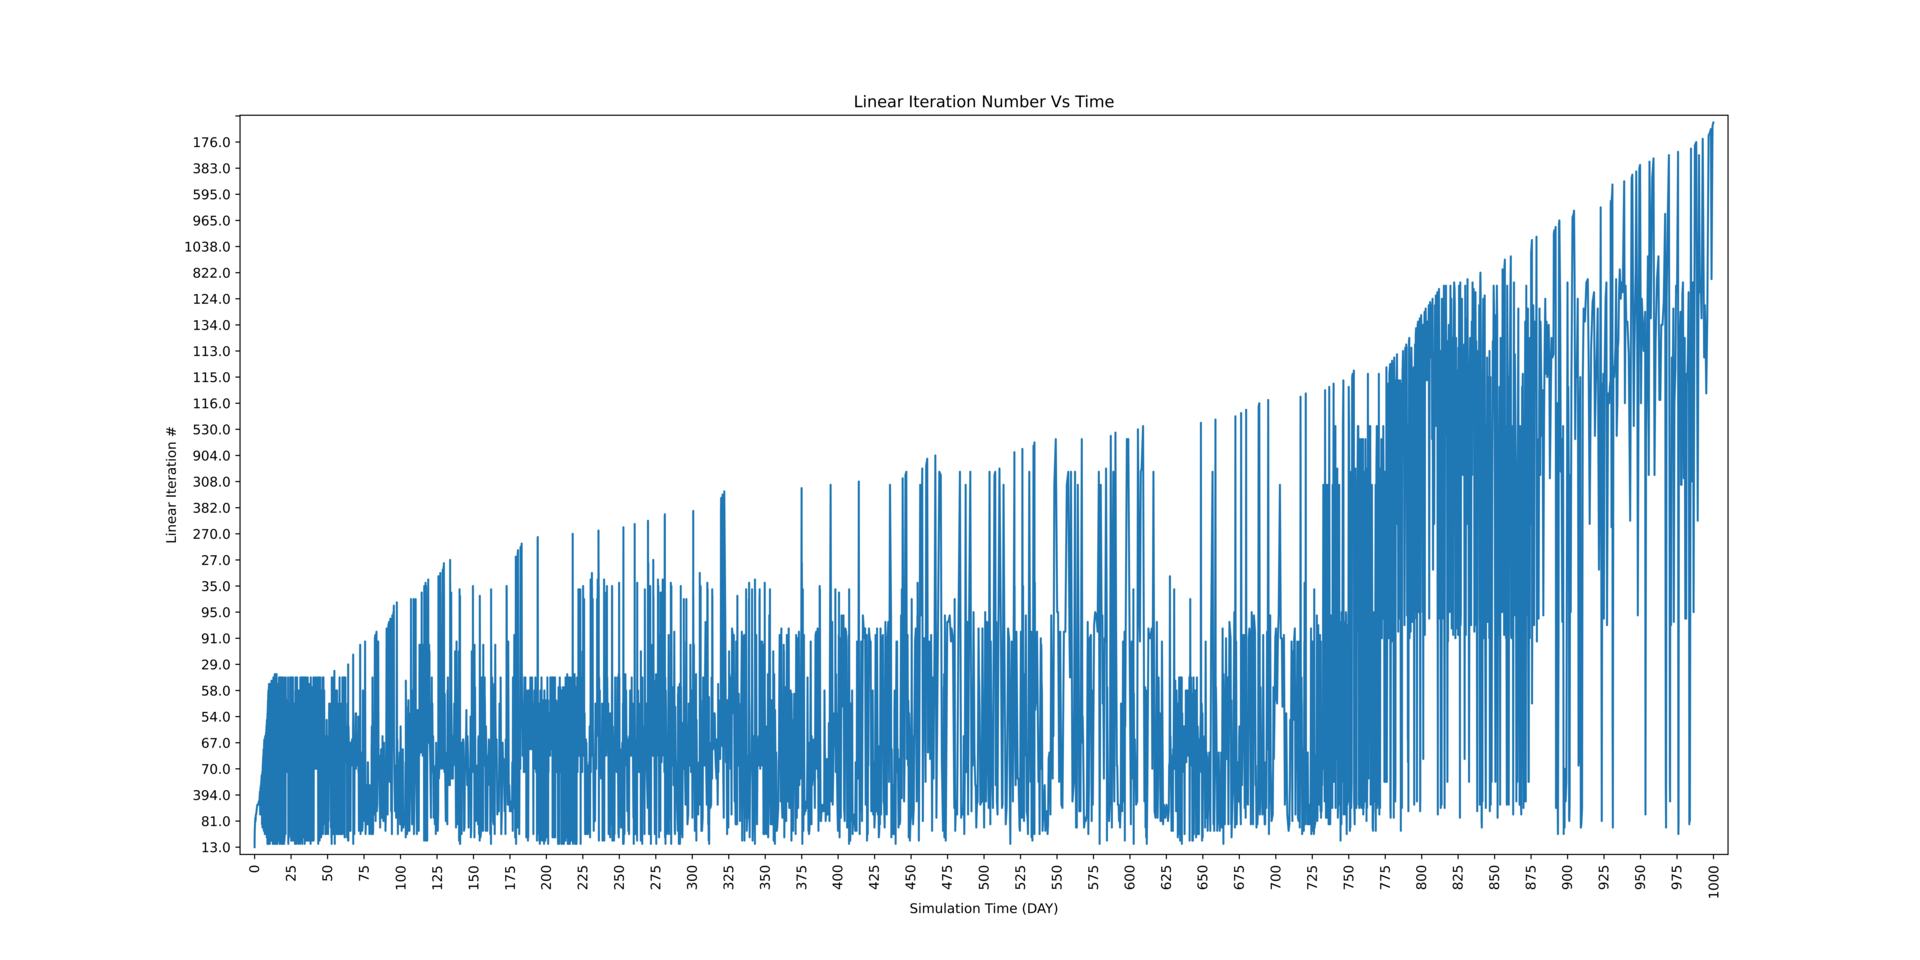
\includegraphics[width=1.1\linewidth]{figures/case9/ilu/its_time.png_reduced.png}
  \caption{\texttt{GMRES-ILU(0)} preconditioner}
	\label{case9_its_ilu}
\end{subfigure}
\begin{subfigure}{.5\textwidth}
  \centering
  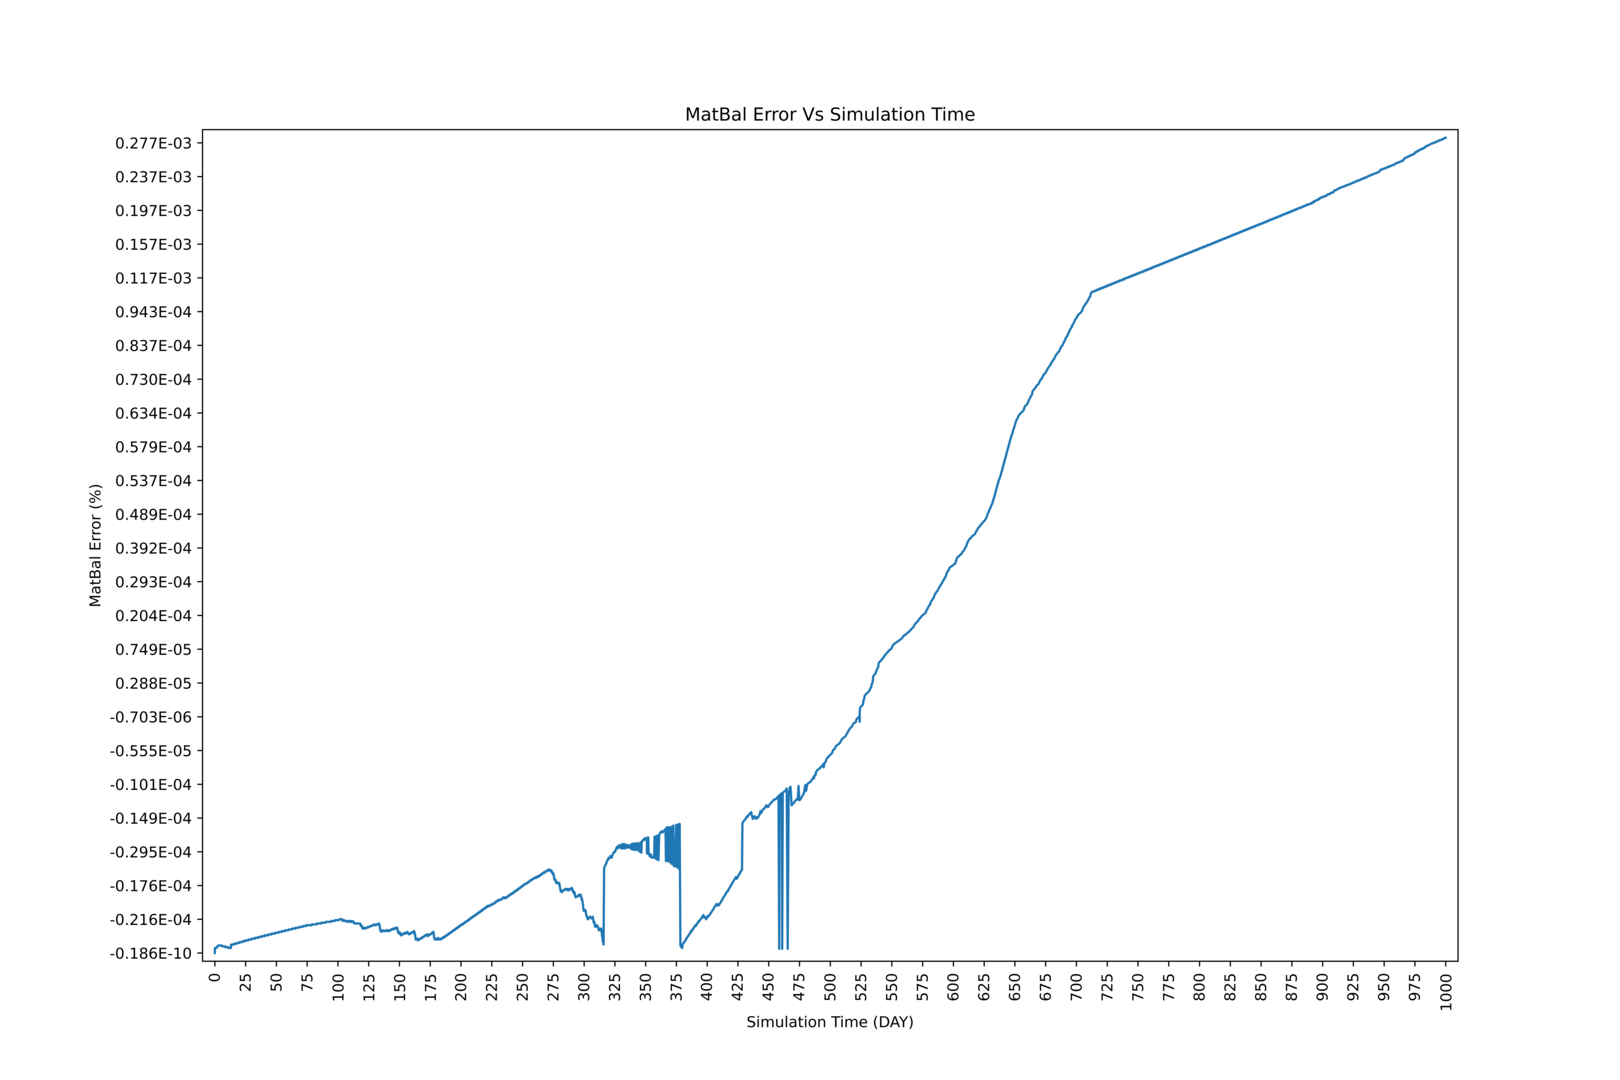
\includegraphics[width=1.1\linewidth]{figures/case9/cpr/matbalerr_time.png_reduced.png}
  \caption{\texttt{CPR-AMG} preconditioner.}
	\label{case9_matbalerr_cpr}
\end{subfigure}%
\begin{subfigure}{.5\textwidth}
  \centering
  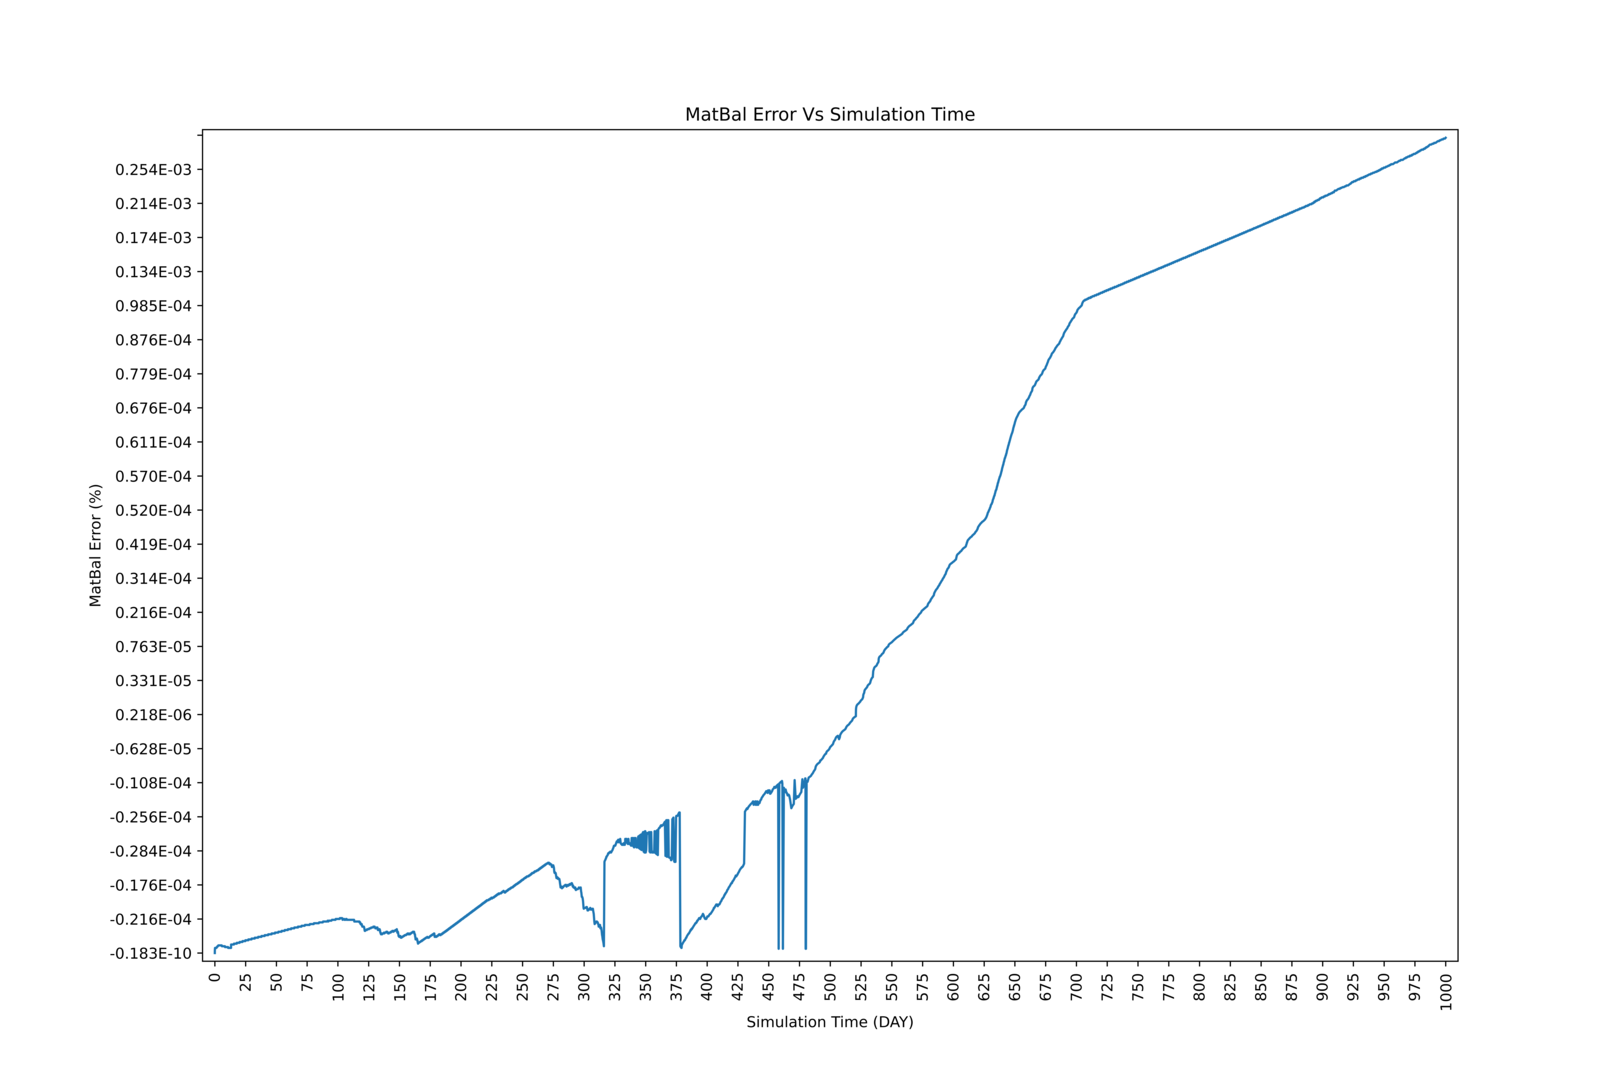
\includegraphics[width=1.1\linewidth]{figures/case9/ilu/matbalerr_time.png_reduced.png}
  \caption{\texttt{GMRES-ILU(0)} preconditioner}
	\label{case9_matbalerr_ilu}
\end{subfigure}
\caption[caption]{A comparison for \texttt{Case 5} for the two different preconditioning methods.\\\hspace{\textwidth}
		\cref{case9_cpu_cpr,case9_cpu_ilu}: CPU run time against simulation time. \\\hspace{\textwidth}
		\cref{case9_its_cpr,case9_its_ilu}: Linear iterations against simulation time.\\\hspace{\textwidth}
		\cref{case9_matbalerr_cpr,case9_matbalerr_ilu}: Material balance error against simulation time.}
\label{case9sg}
\end{figure}
\clearpage

\section{Case 6}
This simulation model is a modified version of a study of how compositional effects contribute to oil displacement by CO$_{2}$\supercite{case6paper}.
The modification is done to investigate grid refinement. The simulation grid was refined to $20\times20$, $80\times80$ and $320\times320$.
The heterogeneity of porosity and permeability were altered from those published in the paper to allow for viscous fingering.
This simulation problem was the most intresting case for the CPR preconditioner, since the default \texttt{ILU(0)-GMRES} solver-preconditioner combination
could not finish the simulation in less than a day for the ($320\times320$) scenario, when CPR managed to finish it within 12.68 hours. 

\FloatBarrier
\begin{center}
\begin{table}[h!]
\begin{adjustbox}{width=0.5\textwidth}
    \begin{threeparttable}
    \caption{\textbf{Case 4 Reservoir Parameters\supercite{phdfernandes}.}}
    \label{case4}
        \begin{tabular}{l r }
            \toprule
            Simulatoin Parameters & Value\\
            \midrule
	\rowcolor{red!20}\textit{\textbf{Reservoir data}}      & \\
	Grid:      &            \\
	\rowcolor{blue!5}Number of wells:      &  2 (1 injector / 1 producer) \\
	Length, width and thickness:      & \\
	\rowcolor{blue!5}Porosity:       &           \\
	Permeability ($X, \ Y, \ Z$) &  mD\\
	\rowcolor{blue!5}Initial water saturation:    &  \\      
	Formation temperature:    &  F$^{\circ}$     \\
	\rowcolor{blue!5}Initial pressure:    &       psi\\
	Reservoir’s initial composition () & \\
        \bottomrule
        \end{tabular}
    \end{threeparttable}
\end{adjustbox}    
\end{table}
\end{center}
\FloatBarrier

\begin{table}[h!]
   \caption{Comparison parameters for \texttt{Case 6}.}
   \label{case6-tab}
   \small
   \centering
   \begin{tabular}{lcc}
   \toprule\toprule
   \textbf{Variable} & \textbf{CPR-AMG} & \textbf{GMRES-ILU(0)} \\
   \midrule
   CPU Time (hr) & 12.67 &  NA \\
   Solver Time (hr) & 7.2  & NA \\
   \# Newton Iterations & 14,695 & NA\\
   \# Solver Iterations & 167,070 & NA \\
   \# Time Steps & 4,011& NA \\
   \bottomrule
   \end{tabular}
\end{table}

\begin{figure}[h!]
\centering
\begin{subfigure}{.5\textwidth}
  \centering
  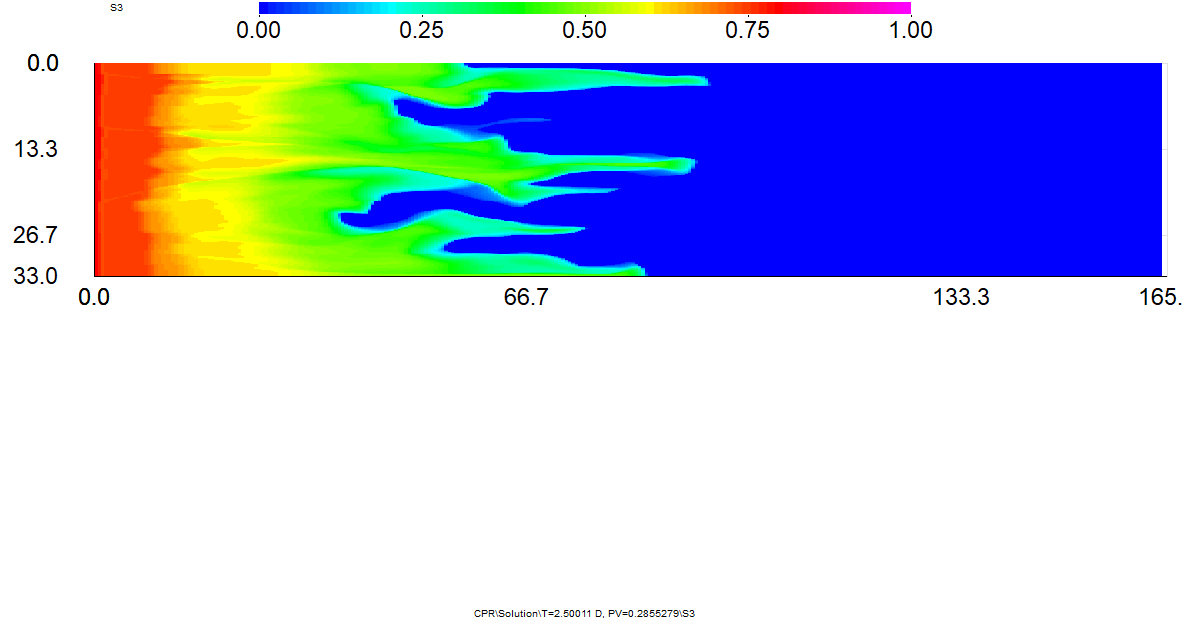
\includegraphics[width=1\linewidth]{figures/case6_cpr_sg.png}
  \caption{\texttt{CPR-AMG} preconditioner.}
\end{subfigure}%
\begin{subfigure}{.5\textwidth}
  \centering
  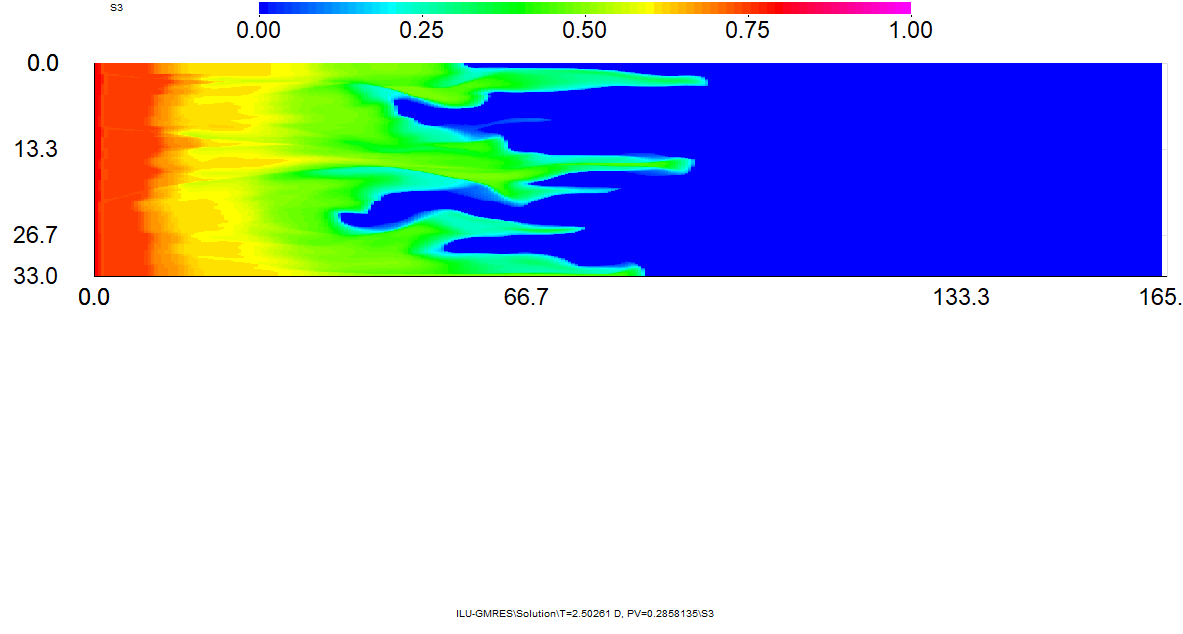
\includegraphics[width=1\linewidth]{figures/case6_ilu_sg.png}
  \caption{\texttt{GMRES-ILU(0)} preconditioner}
\end{subfigure}
\caption{A comparison of \texttt{Case 6} gas saturation $S_{g}$ distribution for the two different preconditioning methods after 2.5 days of simulation time.}
\label{case5sg}
\end{figure}

\begin{figure}[h!]
\centering
\begin{subfigure}{.5\textwidth}
  \centering
  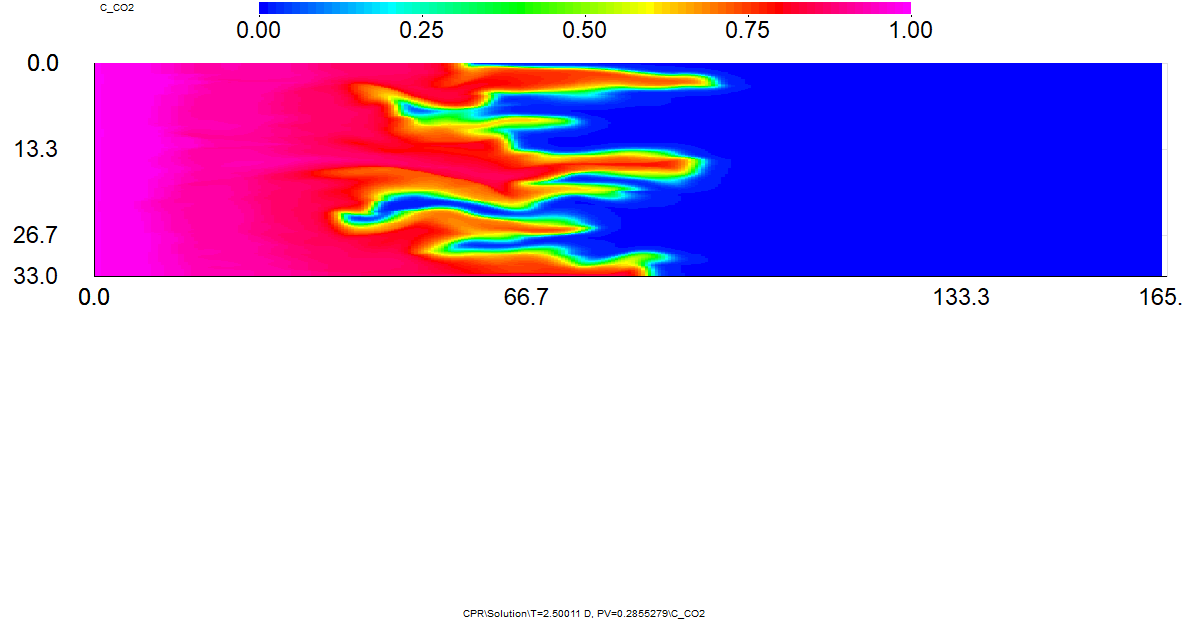
\includegraphics[width=1\linewidth]{figures/case6_cpr_co2.png}
  \caption{\texttt{CPR-AMG} preconditioner.}
\end{subfigure}%
\begin{subfigure}{.5\textwidth}
  \centering
  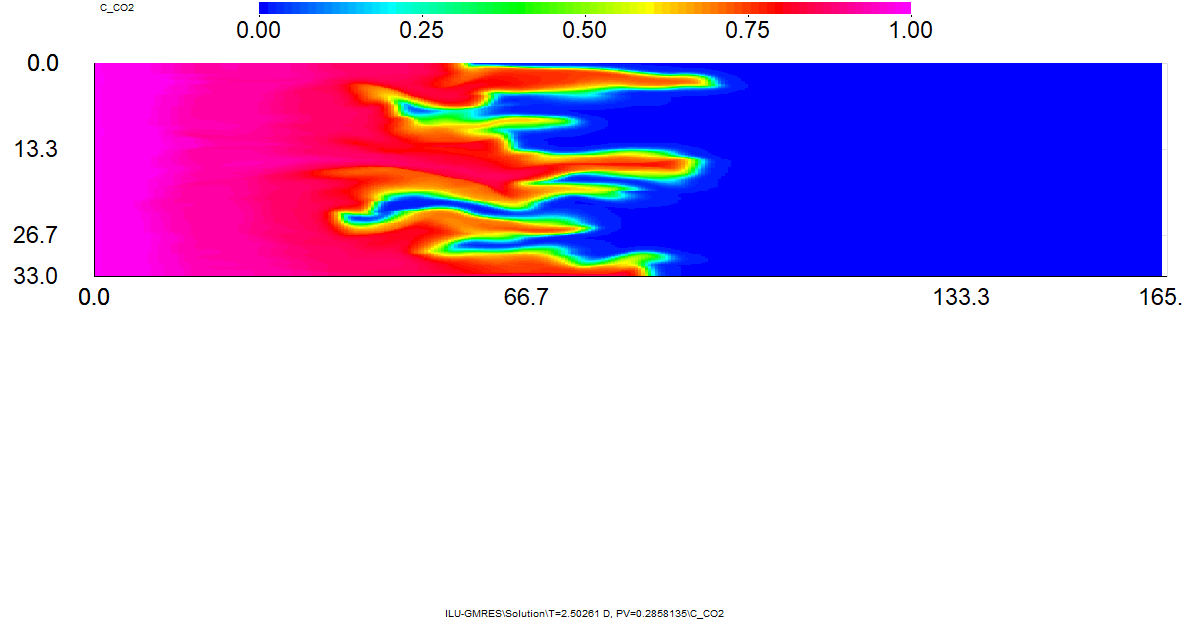
\includegraphics[width=1\linewidth]{figures/case6_ilu_co2.png}
  \caption{\texttt{GMRES-ILU(0)} preconditioner}
\end{subfigure}
\caption{A comparison of \texttt{Case 6} CO$_{2}$ saturation $S_{g}$ distribution for the two different preconditioning methods after 2.5 days of simulation time.}
\label{case5sg}
\end{figure}


 \chapter{Conclusion}
Preconditioning refers to any modifications of the original system of equations with the purpose of enhancing the performance of
the iterative solver that will solve the system. Physics based precondtioning refers to the decoupling of the blocks in the jacobian
matrix based on the nature of the variables and applying the appropriate preconditioner for each variable based on the nature of its equation.
By recoginizing the global nature of the pressure variable, that is a change of pressure in a gridblock will effect the
global domain of the reservoir, and the local nature of the concentraion or saturation variables, physically based preconditioner can be devised
to treat each variable sperately. In reservoir simulation, these preconditioning techniques are refered to as two-stage precondtioners.
The overall results of this report show that for compositional models, with a large number of component (more than 4), 
the \textit{constrained pressure residual} preconditioner outperform the \textit{Incomplete Lower-Upper(0)} preconditioner 
with \texttt{GMRES} as a Krylov solver. The research literature in reservoir simulation has further developed the CPR preconditioner, 
since its appearance in 1985 \cite{Wallis_1985}. The improvements include the implementation of several decoupling techniques, combining
CPR with Algebraic Multigrid as a precondtioner for the resulting pressure subsystem and the extension of CPR to handle thermal models by
developing \textit{Constrained Pressure-Temperature Residual}(CPTR) preconditioner \cite{cptr}.
Possible further investigations in this area can be applying CPR on adaptive-implicit formulations. Based on the degree of implicitness of the
system such preconditioning techniques may or may not be effective. 



%%% Appendicies of thesis  %%%%%%%%%%%%%%%%%%%%%%%%%%%%%%%%%%%%%%%%%%%%%%%%%%%%%%%%%%%%%%%%%%%%%%%%

\cleardoublepage\makeatletter\@openrightfalse\makeatother
\appendix
% From mitthesis package
% Version: 1.01, 2023/07/04
% Documentation: https://ctan.org/pkg/mitthesis


\chapter{Code listing}

\lstset{language=[90]Fortran,
  basicstyle=\tiny\ttfamily,
  keywordstyle=\color{red},
  commentstyle=\color{Blue3},
  morecomment=[l]{!\ }% Comment only with space after !
  numberstyle=\tiny\color{gray},
  backgroundcolor=\color{CadetBlue!15!white},   
  numbers=left,                    
  numbersep=5pt,                  
}

\begin{lstlisting}
    Module CPR_Precond 
    use modulepetsc
    use modulecom, only: NCP1, NB
    use cfuncs
    USE PETSC
    USE MODULEFIMF, only: NWSIZE
    use MODULEPARA, only: NWM, NWBCM
    use MODULEGENFRAME, only: maxStencil
#include "petsc/finclude/petsc.h"
#include "petsc/finclude/petscsys.h"

    implicit none
    
    type, public :: cpr_ctx
            Mat :: A, Ap 
            Vec :: r, x, rp, xp, s1, s2
            KSP :: ksp, ksp_p
            PC  :: pc_1, pc_2
            integer :: decoupler
            real    :: t1, t2
            real    :: dec_t, sol_t
    end type
    
    public      :: cpr_init
    public      :: cpr_apply
    private     :: QIMPES_dec
    private     :: ABF_dec
    public      :: cpr_reset_ksp 
    type(cpr_ctx), public :: ctx

    interface
        subroutine PCShellSetContext(pc, ctx, ierr)
        use petscksp
        import :: cpr_ctx
        PC :: pc
        type(cpr_ctx) :: ctx
        integer :: ierr
        end subroutine
    end interface

    interface
        subroutine PCShellGetContext(pc, ctx, ierr)
        use petscksp
        import :: cpr_ctx
        PC :: pc
        type(cpr_ctx), pointer :: ctx
        integer :: ierr
        end subroutine
    end interface

    contains

    subroutine cpr_init(ctx)
    ! CPR is a two-stage preconditioner. The first preconditioner is used
    ! to solve the pressure subsystem (using GMRES or AMG), the second is used to 
    ! solve the combined preconditioned pressure and saturation system 
    ! (using ILU).

    integer :: ierr
    type(cpr_ctx) :: ctx
    PC :: prec
    PetscInt :: nrows, ncols

    NWSIZE = NWM*NWBCM*NCP1
    nrows = NB*NCP1 + NWSIZE
    ncols = nrows
    ctx%dec_t = 0
    ctx%sol_t = 0
    !!!!!!!!!!!!!!!!!!!!!!!!!!!!!!!!!!!!!!!!!!!!!!!!!!!!!!!!!!!!!!!!!!!!!!!
    ! Create matrices and vectors used in CPR solver                      !
    !!!!!!!!!!!!!!!!!!!!!!!!!!!!!!!!!!!!!!!!!!!!!!!!!!!!!!!!!!!!!!!!!!!!!!!
    call VecCreateSeq(PETSC_COMM_WORLD, nrows, ctx%r, ierr)
    call VecSetBlockSize(ctx%r, NCP1, ierr)
    call VecSetUp(ctx%r, ierr)
    call VecDuplicate(ctx%r, ctx%x, ierr)
    call VecDuplicate(ctx%r, ctx%s1, ierr)
    call VecDuplicate(ctx%r, ctx%s2, ierr)
    call MatCreate(PETSC_COMM_WORLD, ctx%A, ierr)
    call MatSetType(ctx%A, MATSEQAIJ, ierr)
    call MatSetSizes(ctx%A, PETSC_DECIDE, PETSC_DECIDE, nrows, ncols, ierr)

    call VecCreateSeq(PETSC_COMM_WORLD, nrows/NCP1, ctx%rp, ierr)
    call VecDuplicate(ctx%rp, ctx%xp, ierr)
    call MatCreate(PETSC_COMM_WORLD, ctx%Ap, ierr)
    call MatSetSizes(ctx%Ap, PETSC_DECIDE, PETSC_DECIDE, nrows/NCP1, nrows/NCP1, ierr)
    call MatSetUp(ctx%Ap, ierr)

    !!!!!!!!!!!!!!!!!!!!!!!!!!!!!!!!!!!!!!!!!!!!!!!!!!!!!!!!!!!!!!!!!!!!!!!
    ! Create the whole system krylov solver                               !
    !!!!!!!!!!!!!!!!!!!!!!!!!!!!!!!!!!!!!!!!!!!!!!!!!!!!!!!!!!!!!!!!!!!!!!!
    call KSPCreate(PETSC_COMM_WORLD, ctx%ksp, ierr)
    call KSPSetType(ctx%ksp, KSPFGMRES, ierr)
    call KSPSetOperators(ctx%ksp, ctx%A, ctx%A, ierr)
    call KSPGetPc(ctx%ksp, ctx%pc_1, ierr)
    call PCSetType(ctx%pc_1, PCSHELL, ierr)
    call PCShellSetApply(ctx%pc_1, cpr_apply, ierr)
    call PCShellSetContext(ctx%pc_1, ctx, ierr)
    !!!!!!!!!!!!!!!!!!!!!!!!!!!!!!!!!!!!!!!!!!!!!!!!!!!!!!!!!!!!!!!!!!!!!!!
    ! Create the first stage (inner) preconditioner.                      !
    !!!!!!!!!!!!!!!!!!!!!!!!!!!!!!!!!!!!!!!!!!!!!!!!!!!!!!!!!!!!!!!!!!!!!!!
    call KSPCreate(PETSC_COMM_WORLD, ctx%ksp_p, ierr)
    !call KSPSetType(ctx%ksp_p, KSPGMRES, ierr)
    call KSPSetType(ctx%ksp_p, KSPPREONLY, ierr)
    call KSPGetPc(ctx%ksp_p, prec, ierr)
    !call PCSetType(prec, PCNONE, ierr)
    call PCSetType(prec, PCHYPRE, ierr)
    call PCHYPRESetType(prec, "boomeramg", ierr)

    call KSPSetOperators(ctx%ksp_p, ctx%Ap, ctx%Ap, ierr)
    !!!!!!!!!!!!!!!!!!!!!!!!!!!!!!!!!!!!!!!!!!!!!!!!!!!!!!!!!!!!!!!!!!!!!!!
    ! Create the second stage (outter) preconditioner.                    !
    !!!!!!!!!!!!!!!!!!!!!!!!!!!!!!!!!!!!!!!!!!!!!!!!!!!!!!!!!!!!!!!!!!!!!!!
    call PCCreate(PETSC_COMM_WORLD, ctx%pc_2, ierr)
    call PCSetType(ctx%pc_2, PCILU, ierr)
    call PCSetOperators(ctx%pc_2, ctx%A, ctx%A, ierr)
    end subroutine

    subroutine cpr_apply(pc, res, res_o, ierr)
    PC          :: pc, amg
    Vec         :: res, res_o
    Vec         :: r2
    integer     :: ierr 
    type(cpr_ctx), pointer :: ctx
    Mat         :: pfmat, pfap
    Vec         :: pfrhs, pfrp

    call PCShellGetContext(pc, ctx, ierr)

    !!!!!!!!!!!!!!!!!!!!!!!!!!!!!!!!!!!!!!!!!!!!!!!!!!!!!!!!!!!!!!!!!!!!!!!
    ! Apply the first stage (inner) preconditioner.                       !
    !!!!!!!!!!!!!!!!!!!!!!!!!!!!!!!!!!!!!!!!!!!!!!!!!!!!!!!!!!!!!!!!!!!!!!!
    call cpu_time(ctx%t1)
    call ABF_dec(ctx%A, res, ctx%Ap, ctx%rp)
    call cpu_time(ctx%t2)
    ctx%dec_t = ctx%dec_t + ctx%t2 - ctx%t1
    call cpu_time(ctx%t1)
    call KSPGetPC(ctx%ksp_p, amg, ierr)
    call PCApply(amg, ctx%rp, ctx%xp, ierr)
    !call KSPSolve(ctx%ksp_p, ctx%rp, ctx%xp, ierr)
    call cpu_time(ctx%t2)
    ctx%sol_t = ctx%sol_t + ctx%t2 - ctx%t1
    call VecZeroEntries(ctx%s1, ierr)
    call VecStrideScatter(ctx%xp, 0, ctx%s1, INSERT_VALUES, ierr)
    !!!!!!!!!!!!!!!!!!!!!!!!!!!!!!!!!!!!!!!!!!!!!!!!!!!!!!!!!!!!!!!!!!!!!!!
    ! Apply the second stage (outter) preconditioner.                     !
    !!!!!!!!!!!!!!!!!!!!!!!!!!!!!!!!!!!!!!!!!!!!!!!!!!!!!!!!!!!!!!!!!!!!!!!
    call MatMult(ctx%A, ctx%s1, ctx%s2, ierr)
    call VecAYPX(ctx%s2, -1.d0, res, ierr)
    call PCApply(ctx%pc_2, ctx%s2, res_o, ierr)
    call VecAYPX(res_o, 1.d0, ctx%s1, ierr)
    end subroutine

    subroutine QIMPES_dec(A, Ap)
    ! The QIMPES decoupler produces the following pressure matrix !
    ! and corresponding residual :                                !
    ! Ap  = App - Aps * Dss * Asp                                 !
    ! rp* = rp - Aps * Dss * rs                                   !
    Mat, intent(in)     :: A, Ap
    integer :: ierr

    end subroutine

    subroutine ABF_dec(A, r, Ap, rp)
    ! The ABF decoupler produces the following pressure matrix  !
    ! and corresponding residual:                               !
    ! Ap  = lambda_inv * (Dss*App - Dps*Asp)                    !
    ! rp* = lambda_inv * (Dss*rp - Dps*rs)                      !
    ! lambda_inv = Dpp*Dss - Dps*Dsp                            !
    Mat, intent(in)     :: A, Ap
    Vec, intent(in)     :: r, rp
    Vec :: diag, mult
    PetscInt            :: i, j, k, ierr, nrows, ncols, rsize
    PetscScalar, dimension(:,:), pointer         :: all_vals 
    PetscScalar, dimension(:), pointer         :: Ap_row, row_vals
    PetscScalar         :: diag_block(0:NCP1-1, 0:NCP1-1)
    PetscInt            :: Ap_colIdx(0:maxval(PNNZD)), nnzr
    PetscInt, dimension(:), pointer     :: colsIdx, ix
    PetscScalar         :: lambda_inv
    integer             :: blk_size, pressEq_row, diag_indx, nblks_row, blk_col 
    integer             :: LWORK, INFO
    integer, dimension(NCP1) :: IPIV
    real, dimension(NCP1) :: WORK

    Ap_colIdx(:) = -1
    blk_size = NCP1
    rsize = maxStencil*NCP1 + NWSIZE
    call MatGetLocalSize(A, nrows, ncols, ierr)
    allocate(all_vals(0:blk_size-1, 0:rsize))
    allocate(Ap_row(0:rsize), row_vals(0:rsize), colsIdx(0:rsize), ix(0:blk_size-1))
    call VecCreate(PETSC_COMM_WORLD, diag, ierr)
    call VecSetType(diag, VECSEQ, ierr)
    call VecSetSizes(diag, PETSC_DECIDE, nrows, ierr)
    call VecSetBlockSize(diag, blk_size, ierr)
    call VecDuplicate(diag, mult, ierr)
    LWORK = blk_size

    ! ============================================================= !
    !                 Main loop over blocks in a row                !
    ! ============================================================= !
    ! loop over the blocked matrix rows to construct Ap, the        !
    ! matrices App, Aps, Asp, Ass, Dpp, Dps, Dsp and Dss are never  !
    ! constructed explicitly, but there corresponding row values    !
    ! are used to build Ap.                                         !
    do i = 0, (nrows/blk_size)-1 !NB-1
        all_vals(:,:) = 0
        row_vals(:) = 0
        colsIdx(:) = 0
        Ap_ColIdx(:) = 0
        ! ======================================== !
        ! Pressure equation extraction             !
        ! ======================================== !
        pressEq_row = i*blk_size
        call MatGetRow(A, pressEq_row, nnzr, colsIdx, row_vals, ierr)
        nblks_row = nnzr/blk_size
        ! loop to get diagonal block column index 
        diag_indx = -1 
        do j = 0, nnzr-1, blk_size !PNNZD(pressEq_row), blk_size
           if(colsIdx(j) == pressEq_row) then
              diag_indx = j
              exit
           endif
        enddo
        ! App and Aps
        all_vals(0, :) = row_vals(:)
        Ap_ColIdx = ColsIdx(0::blk_size)/blk_size
        call MatRestoreRow(A, pressEq_row, nnzr, colsIdx, row_vals, ierr)
        ! ======================================== !
        ! Concentrations equations extraction      !
        ! ======================================== !
        do k = 1, blk_size-1 
           call MatGetRow(A, pressEq_row+k, nnzr, colsIdx, row_vals, ierr)
           ! Asp and Ass
           all_vals(k, :) = row_vals(:)
           call MatRestoreRow(A, pressEq_row+k, nnzr, colsIdx, row_vals, ierr)
        enddo
        ! ======================================== !
        ! Inversion of diagonal blocks             !
        ! ======================================== !
        diag_block = all_vals(:, diag_indx:diag_indx+blk_size-1)
        call DGETRF(blk_size, blk_size, diag_block, blk_size, IPIV, INFO)
        call DGETRI(blk_size, diag_block, blk_size, IPIV, WORK, LWORK, INFO)
        if (INFO > 0) then
                write(*,*) "CPR ABF extraction failed."
                call exit()
        endif
        ! ======================================== !
        ! Ap row to insert                         !
        ! ======================================== !
        Ap_row(:) = 0
        do j=0, nblks_row-1
                blk_col = j*blk_size
                do k=0, blk_size-1
                        Ap_row(j) = Ap_row(j) + diag_block(0, k) * all_vals(k, blk_col)
                        ix(k) = pressEq_row + k
                enddo
        enddo
        call MatSetValues(Ap, 1, i, nblks_row, Ap_ColIdx(0:nblks_row-1), Ap_row(0:nblks_row-1), INSERT_VALUES, ierr)
        call VecSetValues(diag, blk_size, ix, diag_block(0,:), INSERT_VALUES, ierr)
    enddo
    call MatAssemblyBegin(Ap, MAT_FINAL_ASSEMBLY, ierr)
    call MatAssemblyEnd(Ap, MAT_FINAL_ASSEMBLY, ierr)
    call VecAssemblyBegin(diag, ierr)
    call VecAssemblyEnd(diag, ierr)

    call VecPointwiseMult(mult,diag,r,ierr)
    k = 0
    call VecStrideGather(mult,k,rp,INSERT_VALUES,ierr)
    do k = 1,blk_size-1
        call VecStrideGather(mult,k,rp,ADD_VALUES,ierr)
    enddo
    end subroutine

    subroutine cpr_reset_ksp(ctx)
    integer :: ierr
    type(cpr_ctx) :: ctx
    call KSPDestroy(ctx%ksp_p, ierr)
    call PCDestroy(ctx%pc_2, ierr)
    call cpr_init(ctx)
    end subroutine

    END Module
\end{lstlisting}

%% From mitthesis package
% Version: 1.01, 2023/07/04
% Documentation: https://ctan.org/pkg/mitthesis


\chapter{Code listing}

\lstset{language=[90]Fortran,
  basicstyle=\tiny\ttfamily,
  keywordstyle=\color{red},
  commentstyle=\color{Blue3},
  morecomment=[l]{!\ }% Comment only with space after !
  numberstyle=\tiny\color{gray},
  backgroundcolor=\color{CadetBlue!15!white},   
  numbers=left,                    
  numbersep=5pt,                  
}

\begin{lstlisting}
    Module CPR_Precond 
    use modulepetsc
    use modulecom, only: NCP1, NB
    use cfuncs
    USE PETSC
    USE MODULEFIMF, only: NWSIZE
    use MODULEPARA, only: NWM, NWBCM
    use MODULEGENFRAME, only: maxStencil
#include "petsc/finclude/petsc.h"
#include "petsc/finclude/petscsys.h"

    implicit none
    
    type, public :: cpr_ctx
            Mat :: A, Ap 
            Vec :: r, x, rp, xp, s1, s2
            KSP :: ksp, ksp_p
            PC  :: pc_1, pc_2
            integer :: decoupler
            real    :: t1, t2
            real    :: dec_t, sol_t
    end type
    
    public      :: cpr_init
    public      :: cpr_apply
    private     :: QIMPES_dec
    private     :: ABF_dec
    public      :: cpr_reset_ksp 
    type(cpr_ctx), public :: ctx

    interface
        subroutine PCShellSetContext(pc, ctx, ierr)
        use petscksp
        import :: cpr_ctx
        PC :: pc
        type(cpr_ctx) :: ctx
        integer :: ierr
        end subroutine
    end interface

    interface
        subroutine PCShellGetContext(pc, ctx, ierr)
        use petscksp
        import :: cpr_ctx
        PC :: pc
        type(cpr_ctx), pointer :: ctx
        integer :: ierr
        end subroutine
    end interface

    contains

    subroutine cpr_init(ctx)
    ! CPR is a two-stage preconditioner. The first preconditioner is used
    ! to solve the pressure subsystem (using GMRES or AMG), the second is used to 
    ! solve the combined preconditioned pressure and saturation system 
    ! (using ILU).

    integer :: ierr
    type(cpr_ctx) :: ctx
    PC :: prec
    PetscInt :: nrows, ncols

    NWSIZE = NWM*NWBCM*NCP1
    nrows = NB*NCP1 + NWSIZE
    ncols = nrows
    ctx%dec_t = 0
    ctx%sol_t = 0
    !!!!!!!!!!!!!!!!!!!!!!!!!!!!!!!!!!!!!!!!!!!!!!!!!!!!!!!!!!!!!!!!!!!!!!!
    ! Create matrices and vectors used in CPR solver                      !
    !!!!!!!!!!!!!!!!!!!!!!!!!!!!!!!!!!!!!!!!!!!!!!!!!!!!!!!!!!!!!!!!!!!!!!!
    call VecCreateSeq(PETSC_COMM_WORLD, nrows, ctx%r, ierr)
    call VecSetBlockSize(ctx%r, NCP1, ierr)
    call VecSetUp(ctx%r, ierr)
    call VecDuplicate(ctx%r, ctx%x, ierr)
    call VecDuplicate(ctx%r, ctx%s1, ierr)
    call VecDuplicate(ctx%r, ctx%s2, ierr)
    call MatCreate(PETSC_COMM_WORLD, ctx%A, ierr)
    call MatSetType(ctx%A, MATSEQAIJ, ierr)
    call MatSetSizes(ctx%A, PETSC_DECIDE, PETSC_DECIDE, nrows, ncols, ierr)

    call VecCreateSeq(PETSC_COMM_WORLD, nrows/NCP1, ctx%rp, ierr)
    call VecDuplicate(ctx%rp, ctx%xp, ierr)
    call MatCreate(PETSC_COMM_WORLD, ctx%Ap, ierr)
    call MatSetSizes(ctx%Ap, PETSC_DECIDE, PETSC_DECIDE, nrows/NCP1, nrows/NCP1, ierr)
    call MatSetUp(ctx%Ap, ierr)

    !!!!!!!!!!!!!!!!!!!!!!!!!!!!!!!!!!!!!!!!!!!!!!!!!!!!!!!!!!!!!!!!!!!!!!!
    ! Create the whole system krylov solver                               !
    !!!!!!!!!!!!!!!!!!!!!!!!!!!!!!!!!!!!!!!!!!!!!!!!!!!!!!!!!!!!!!!!!!!!!!!
    call KSPCreate(PETSC_COMM_WORLD, ctx%ksp, ierr)
    call KSPSetType(ctx%ksp, KSPFGMRES, ierr)
    call KSPSetOperators(ctx%ksp, ctx%A, ctx%A, ierr)
    call KSPGetPc(ctx%ksp, ctx%pc_1, ierr)
    call PCSetType(ctx%pc_1, PCSHELL, ierr)
    call PCShellSetApply(ctx%pc_1, cpr_apply, ierr)
    call PCShellSetContext(ctx%pc_1, ctx, ierr)
    !!!!!!!!!!!!!!!!!!!!!!!!!!!!!!!!!!!!!!!!!!!!!!!!!!!!!!!!!!!!!!!!!!!!!!!
    ! Create the first stage (inner) preconditioner.                      !
    !!!!!!!!!!!!!!!!!!!!!!!!!!!!!!!!!!!!!!!!!!!!!!!!!!!!!!!!!!!!!!!!!!!!!!!
    call KSPCreate(PETSC_COMM_WORLD, ctx%ksp_p, ierr)
    !call KSPSetType(ctx%ksp_p, KSPGMRES, ierr)
    call KSPSetType(ctx%ksp_p, KSPPREONLY, ierr)
    call KSPGetPc(ctx%ksp_p, prec, ierr)
    !call PCSetType(prec, PCNONE, ierr)
    call PCSetType(prec, PCHYPRE, ierr)
    call PCHYPRESetType(prec, "boomeramg", ierr)

    call KSPSetOperators(ctx%ksp_p, ctx%Ap, ctx%Ap, ierr)
    !!!!!!!!!!!!!!!!!!!!!!!!!!!!!!!!!!!!!!!!!!!!!!!!!!!!!!!!!!!!!!!!!!!!!!!
    ! Create the second stage (outter) preconditioner.                    !
    !!!!!!!!!!!!!!!!!!!!!!!!!!!!!!!!!!!!!!!!!!!!!!!!!!!!!!!!!!!!!!!!!!!!!!!
    call PCCreate(PETSC_COMM_WORLD, ctx%pc_2, ierr)
    call PCSetType(ctx%pc_2, PCILU, ierr)
    call PCSetOperators(ctx%pc_2, ctx%A, ctx%A, ierr)
    end subroutine

    subroutine cpr_apply(pc, res, res_o, ierr)
    PC          :: pc, amg
    Vec         :: res, res_o
    Vec         :: r2
    integer     :: ierr 
    type(cpr_ctx), pointer :: ctx
    Mat         :: pfmat, pfap
    Vec         :: pfrhs, pfrp

    call PCShellGetContext(pc, ctx, ierr)

    !!!!!!!!!!!!!!!!!!!!!!!!!!!!!!!!!!!!!!!!!!!!!!!!!!!!!!!!!!!!!!!!!!!!!!!
    ! Apply the first stage (inner) preconditioner.                       !
    !!!!!!!!!!!!!!!!!!!!!!!!!!!!!!!!!!!!!!!!!!!!!!!!!!!!!!!!!!!!!!!!!!!!!!!
    call cpu_time(ctx%t1)
    call ABF_dec(ctx%A, res, ctx%Ap, ctx%rp)
    call cpu_time(ctx%t2)
    ctx%dec_t = ctx%dec_t + ctx%t2 - ctx%t1
    call cpu_time(ctx%t1)
    call KSPGetPC(ctx%ksp_p, amg, ierr)
    call PCApply(amg, ctx%rp, ctx%xp, ierr)
    !call KSPSolve(ctx%ksp_p, ctx%rp, ctx%xp, ierr)
    call cpu_time(ctx%t2)
    ctx%sol_t = ctx%sol_t + ctx%t2 - ctx%t1
    call VecZeroEntries(ctx%s1, ierr)
    call VecStrideScatter(ctx%xp, 0, ctx%s1, INSERT_VALUES, ierr)
    !!!!!!!!!!!!!!!!!!!!!!!!!!!!!!!!!!!!!!!!!!!!!!!!!!!!!!!!!!!!!!!!!!!!!!!
    ! Apply the second stage (outter) preconditioner.                     !
    !!!!!!!!!!!!!!!!!!!!!!!!!!!!!!!!!!!!!!!!!!!!!!!!!!!!!!!!!!!!!!!!!!!!!!!
    call MatMult(ctx%A, ctx%s1, ctx%s2, ierr)
    call VecAYPX(ctx%s2, -1.d0, res, ierr)
    call PCApply(ctx%pc_2, ctx%s2, res_o, ierr)
    call VecAYPX(res_o, 1.d0, ctx%s1, ierr)
    end subroutine

    subroutine QIMPES_dec(A, Ap)
    ! The QIMPES decoupler produces the following pressure matrix !
    ! and corresponding residual :                                !
    ! Ap  = App - Aps * Dss * Asp                                 !
    ! rp* = rp - Aps * Dss * rs                                   !
    Mat, intent(in)     :: A, Ap
    integer :: ierr

    end subroutine

    subroutine ABF_dec(A, r, Ap, rp)
    ! The ABF decoupler produces the following pressure matrix  !
    ! and corresponding residual:                               !
    ! Ap  = lambda_inv * (Dss*App - Dps*Asp)                    !
    ! rp* = lambda_inv * (Dss*rp - Dps*rs)                      !
    ! lambda_inv = Dpp*Dss - Dps*Dsp                            !
    Mat, intent(in)     :: A, Ap
    Vec, intent(in)     :: r, rp
    Vec :: diag, mult
    PetscInt            :: i, j, k, ierr, nrows, ncols, rsize
    PetscScalar, dimension(:,:), pointer         :: all_vals 
    PetscScalar, dimension(:), pointer         :: Ap_row, row_vals
    PetscScalar         :: diag_block(0:NCP1-1, 0:NCP1-1)
    PetscInt            :: Ap_colIdx(0:maxval(PNNZD)), nnzr
    PetscInt, dimension(:), pointer     :: colsIdx, ix
    PetscScalar         :: lambda_inv
    integer             :: blk_size, pressEq_row, diag_indx, nblks_row, blk_col 
    integer             :: LWORK, INFO
    integer, dimension(NCP1) :: IPIV
    real, dimension(NCP1) :: WORK

    Ap_colIdx(:) = -1
    blk_size = NCP1
    rsize = maxStencil*NCP1 + NWSIZE
    call MatGetLocalSize(A, nrows, ncols, ierr)
    allocate(all_vals(0:blk_size-1, 0:rsize))
    allocate(Ap_row(0:rsize), row_vals(0:rsize), colsIdx(0:rsize), ix(0:blk_size-1))
    call VecCreate(PETSC_COMM_WORLD, diag, ierr)
    call VecSetType(diag, VECSEQ, ierr)
    call VecSetSizes(diag, PETSC_DECIDE, nrows, ierr)
    call VecSetBlockSize(diag, blk_size, ierr)
    call VecDuplicate(diag, mult, ierr)
    LWORK = blk_size

    ! ============================================================= !
    !                 Main loop over blocks in a row                !
    ! ============================================================= !
    ! loop over the blocked matrix rows to construct Ap, the        !
    ! matrices App, Aps, Asp, Ass, Dpp, Dps, Dsp and Dss are never  !
    ! constructed explicitly, but there corresponding row values    !
    ! are used to build Ap.                                         !
    do i = 0, (nrows/blk_size)-1 !NB-1
        all_vals(:,:) = 0
        row_vals(:) = 0
        colsIdx(:) = 0
        Ap_ColIdx(:) = 0
        ! ======================================== !
        ! Pressure equation extraction             !
        ! ======================================== !
        pressEq_row = i*blk_size
        call MatGetRow(A, pressEq_row, nnzr, colsIdx, row_vals, ierr)
        nblks_row = nnzr/blk_size
        ! loop to get diagonal block column index 
        diag_indx = -1 
        do j = 0, nnzr-1, blk_size !PNNZD(pressEq_row), blk_size
           if(colsIdx(j) == pressEq_row) then
              diag_indx = j
              exit
           endif
        enddo
        ! App and Aps
        all_vals(0, :) = row_vals(:)
        Ap_ColIdx = ColsIdx(0::blk_size)/blk_size
        call MatRestoreRow(A, pressEq_row, nnzr, colsIdx, row_vals, ierr)
        ! ======================================== !
        ! Concentrations equations extraction      !
        ! ======================================== !
        do k = 1, blk_size-1 
           call MatGetRow(A, pressEq_row+k, nnzr, colsIdx, row_vals, ierr)
           ! Asp and Ass
           all_vals(k, :) = row_vals(:)
           call MatRestoreRow(A, pressEq_row+k, nnzr, colsIdx, row_vals, ierr)
        enddo
        ! ======================================== !
        ! Inversion of diagonal blocks             !
        ! ======================================== !
        diag_block = all_vals(:, diag_indx:diag_indx+blk_size-1)
        call DGETRF(blk_size, blk_size, diag_block, blk_size, IPIV, INFO)
        call DGETRI(blk_size, diag_block, blk_size, IPIV, WORK, LWORK, INFO)
        if (INFO > 0) then
                write(*,*) "CPR ABF extraction failed."
                call exit()
        endif
        ! ======================================== !
        ! Ap row to insert                         !
        ! ======================================== !
        Ap_row(:) = 0
        do j=0, nblks_row-1
                blk_col = j*blk_size
                do k=0, blk_size-1
                        Ap_row(j) = Ap_row(j) + diag_block(0, k) * all_vals(k, blk_col)
                        ix(k) = pressEq_row + k
                enddo
        enddo
        call MatSetValues(Ap, 1, i, nblks_row, Ap_ColIdx(0:nblks_row-1), Ap_row(0:nblks_row-1), INSERT_VALUES, ierr)
        call VecSetValues(diag, blk_size, ix, diag_block(0,:), INSERT_VALUES, ierr)
    enddo
    call MatAssemblyBegin(Ap, MAT_FINAL_ASSEMBLY, ierr)
    call MatAssemblyEnd(Ap, MAT_FINAL_ASSEMBLY, ierr)
    call VecAssemblyBegin(diag, ierr)
    call VecAssemblyEnd(diag, ierr)

    call VecPointwiseMult(mult,diag,r,ierr)
    k = 0
    call VecStrideGather(mult,k,rp,INSERT_VALUES,ierr)
    do k = 1,blk_size-1
        call VecStrideGather(mult,k,rp,ADD_VALUES,ierr)
    enddo
    end subroutine

    subroutine cpr_reset_ksp(ctx)
    integer :: ierr
    type(cpr_ctx) :: ctx
    call KSPDestroy(ctx%ksp_p, ierr)
    call PCDestroy(ctx%pc_2, ierr)
    call cpr_init(ctx)
    end subroutine

    END Module
\end{lstlisting}



%%% Bibliography  %%%%%%%%%%%%%%%%%%%%%%%%%%%%%%%%%%%%%%%%%%%%%%%%%%%%%%%%%%%%%%%%%%%%%%%%%%%%%%%%%

\printbibliography[title={References},heading=bibintoc]

% biblatex also supports chapter-by-chapter bibliography, https://tex.stackexchange.com/a/296502/119566
% see the biblatex manual, section 3.14.3


%%%% Option for natbib %%%%%%%%%%%%%

%%   use an appropriate style (.bst) and your own .bib file[s]

%\bibliographystyle{plainnat}
%\bibliography{mitthesis-sample.bib}

\end{document} 
